\documentclass[10pt,a4paper,twoside,headinclude,footinclude,color]{./latex-notes-cls/edoars-notes}
\graphicspath{ {Immagini/} }

\hypersetup{pdfauthor={Edoardo Signorini},
            pdftitle={Topologia generale e algebrica},
            pdfcreator={Latex with hyperref}}

\begin{document}
%MATERIALE INIZIALE
\begin{frontespizio}
\Preambolo{\usepackage{iwona}}
\Universita{Roma Tre}
\Logo{Immagini/logo}
\Facolta{Matematica}
\Scuola{}
\Piede{A.A. 2015--2016, Semestre II}
\Titoletto{Appunti integrativi}
\Titolo{Topologia generale e algebrica}
\Sottotitolo{GE220}
\NCandidato{Di}
\Candidato{Edoardo Signorini}
\end{frontespizio}
\tableofcontents

%MATERIALE PRINCIPALE
%!TEX root = ../main.tex
%%%%%%%%%%%%%%%%%%%%%%%%%%%%%%%%%%%%%%%%%
%
%LEZIONE 22/02/2016 - PRIMA SETTIMANA (1)
%
%%%%%%%%%%%%%%%%%%%%%%%%%%%%%%%%%%%%%%%%%
\chapter{Topologia Generale}

La \emph{topologia} studia gli aspetti geometrici più generali, senza introdurre né strutture algebriche, né metriche, né coordinate.
%%%%%%%%%%%%%%%
%SPAZI METRICI%
%%%%%%%%%%%%%%%
\section{Spazi metrici}

\begin{defn}{Spazio metrico}{spazioMetrico}\index{Spazio!metrico}
    Sia $X\neq\emptyset$ un insieme.
    Diremo che $X$ è uno \emph{spazio metrico} se è definita un'applicazione
    \[
        d\colon X\times X\to\R,(x,y)\mapsto d(x,y),
    \]
    detta \emph{distanza}, che rispetti le seguenti proprietà:
    \begin{description}
        \item[Positività]$d(x,y)\ge 0,\,\fa x,y\in X$ e $d(x,y)=0\iff x=y$;
        \item[Simmetria]$d(x,y)=d(y,x),\,\fa x,y\in X$;
        \item[Triangolare]$d(x,y)\le d(x,z)+d(z,y),\,\fa x,y,z\in X$.
    \end{description}
\end{defn}

\begin{notz}\index{Funzione}
    Da questo momento con \emph{funzione} denoteremo un'applicazione che ha $\R$ come codominio.
\end{notz}

\begin{exe}
    $\R$ è uno spazio metrico, ponendo
    \[
        d(x,y)=\abs{y-x}.
    \]
\end{exe}

\begin{sol}
    \'E sufficiente verificare che le proprietà della definizione \ref{df:spazioMetrico} siano verificate.
    La positività segue banalmente dalla definizione di valore assoluto.
    Per la simmetria osserviamo che
    \[
        d(x,y)=\abs{y-x}=\abs{-(x-y)}=\abs{x-y}=d(y,x).
    \]
    Infine, dal momento che la disuguaglianza triangolare è valida per il valore assoluto, segue
    \[
        d(x,y)=\abs{y-x}=\abs{y-z+z-x}\le\abs{y-z}+\abs{z-x}=d(z,y)+d(x,z).
    \]
\end{sol}

\begin{ese}
    $\R^n$ è uno spazio metrico, ponendo
    \[
        d(\vec{x},\vec{y})=\norma{\vec{y}-\vec{x}}.
    \]
\end{ese}

\begin{ese}
    Sia $X\neq\emptyset$ un insieme qualsiasi, $X$ è uno spazio metrico ponendo
    \[
        d(x,y)= \begin{cases}
            0 & x=y     \\
            1 & x\neq y
        \end{cases},
    \]
    tale applicazione si definisce \emph{distanza discreta}.
\end{ese}

\begin{prop}{Sottoinsieme di uno spazio metrico è uno spazio metrico}{}
    Sia $(X,d)$ uno spazio metrico e sia $Y\subset X$, allora:
    $(Y,\left. d\right|_Y)$ è uno spazio metrico, con
    \[
        \left. d\right|_Y\colon Y\times Y\to\R,(y',y'')\mapsto d(y',y'').
    \]
\end{prop}

\begin{proof}
    $(X,d)$ è uno spazio metrico, quindi per definizione $d$ costituisce una distanza su $X$. Consideriamo quindi la restrizione $\left. d\right|_Y$ di $d$ su $Y$, tale applicazione soddisfa necessariamente le proprietà della distanza in quanto è definita a partire da $d$. Pertanto $(Y,\left. d\right|_Y)$ è uno spazio metrico.
\end{proof}

\begin{notz}
    $\left. d\right|_Y$ di definisce \emph{distanza indotta}.
\end{notz}

\begin{defn}{Sottospazio metrico}{sottospazioMetrico}\index{Sottospazio!metrico}
    Sia $(X,d)$ uno spazio metrico e sia $Y\subset X$.
    $(Y,\left. d\right|_Y)$ si definisce \emph{sottospazio metrico} di $(X,d)$.
\end{defn}

\begin{defn}{Applicazione continua tra spazi metrici}{applContinuaSpMet}\index{Applicazione continua!tra spazi metrici}
    Siano $(X,d_X)$ e $(Y,d_Y)$ due spazi metrici. Un'applicazione $f\colon (X,d_X)\to (Y,d_Y)$ si dice \emph{continua} se, comunque preso $x_0\in X$
    \[
        \fa\e >0\,\ex\d=\d(\e)>0\text{ tale che }d_X(x,x_0)<\d\implies d_Y\big(f(x),f(x_0)\big)<\e.
    \]
\end{defn}

\begin{exe}[per casa]
    Si dimostri che ogni applicazione costante tra spazi metrici è continua.
\end{exe}

\begin{sol}
    Siano $(X,d_X)$ e $(Y,d_Y)$ spazi metrici, definiamo quindi una generica applicazione costante
    \[
        f\colon X\to Y,x\mapsto y_0\in Y,
    \]
    con $y_0$ fissato.
    Sia ora $x_0\in X$ e fissiamo $\e >0$, osserviamo quindi che, preso un qualsiasi $x\in X$, avremo
    \[
        d_Y\big(f(x),f(x_0)\big)=d_Y(y_0,y_0)=0<\e,
    \]
    indipendentemente da $d_X(x,x_0)$.
    Dalla definizione \ref{df:applContinuaSpMet} segue quindi che $f$ è continua.
\end{sol}

\begin{exe}[per casa]
    Sia $(X,d)$ uno spazio metrico, si dimostri che $id_X\colon X\to X,x\mapsto x$ è continua.
\end{exe}

\begin{sol}
    Sia $x_0\in X$ e fissiamo $\e >0$, poniamo quindi $\d>0$ tale che $\d < \e$, da cui
    \[
        d(x,x_0)<\d\implies d\big(id(x),id(x_0)\big)=d(x,x_0)<\d<\e,
    \]
    ovvero $f$ è continua.
\end{sol}
%%%%%%%%%%%%%%%%
%INSIEMI APERTI%
%%%%%%%%%%%%%%%%
\section{Insiemi aperti}

\begin{defn}{Disco aperto}{discoAperto}\index{Disco aperto}
    Sia $(X,d)$ uno spazio metrico. Sia $x\in X$ e sia $r>0$.
    Si definisce \emph{disco aperto} di centro $x$ e raggio $r$, il sottoinsieme di $X$ di tutti i punti la cui distanza da $x$ è inferiore ad $r$:
    \[
        D_x(r)=\Set{y\in X | d(y,x)<r}.
    \]
\end{defn}

\begin{ese}
    Su $\big(\R,\abs{.}\big)$ i dischi aperti di centro $x$ e raggio $r$ sono gli intervalli aperti $(x-r,x+r)$.
\end{ese}

\begin{ese}
    Su $\big(\R^n,\norma{.}\big)$ i dischi aperti sono palle aperte.
\end{ese}

\begin{defn}{Insieme aperto}{aperto}\index{Insieme!aperto}
    Sia $(X,d)$ uno spazio metrico e sia $A\subset X$.
    $A$ è un insieme aperto se può essere scritto come unione di dischi aperti.
\end{defn}

\begin{oss}
    Equivalentemente possiamo definire $A$ aperto se
    \[
        \fa x\in A\,\ex r>0:D_x(r)\subset A,
    \]
    infatti basterà mostrare che
    \[
        A=\bigcup_{x\in A}D_x(r).
    \]
    \graffito{$\subseteq$}Sia $z\in A$, avremo quindi $z\in D_z(r)\implies z\in\bigcup_{x\in A}D_x(r)$;

    \graffito{$\supseteq$}Sia $z\in\bigcup_{x\in A}D_x(r)$, per cui $z\in D_z(r)$, ma per ipotesi $D_z(r)\subset A$, ovvero $z\in A$.
\end{oss}

\begin{ese}
    Sono aperti di $\big(\R,\abs{.}\big)$ i seguenti:
    \begin{itemize}
        \item $\displaystyle{\R=\bigcup_{n\in \Z} D_n(1)}$, oppure $\displaystyle{\R=\bigcup_{n\in \Z} D_0(n)}$;
        \item $\emptyset$;
        \item $(a,b)=D_c(\frac{b-a}{2})$, dove $c=\frac{a+b}{2}$ è il punto medio fra $a,b$;
        \item $(a,+\infty)$;
        \item $(-\infty,b)$.
    \end{itemize}
\end{ese}

\begin{ese}
    Non sono aperti di $\big(\R,\abs{.}\big)$ i seguenti:
    \begin{itemize}
        \item Insiemi finiti;
        \item $\Z$;
        \item $\Q$;
        \item $\R\setminus\Q$.
    \end{itemize}
\end{ese}

\begin{exe}[per casa]
    Su $\big(\R,\abs{.}\big)$ si dimostri che un intervallo chiuso $[a,b]$ non è un insieme aperto.
\end{exe}

\begin{sol}
    Se per assurdo $[a,b]$ fosse aperto, avremmo che
    \[
        \fa x\in [a,b]\,\ex r>0:D_x(r)\subset [a,b],
    \]
    in particolare $\ex r>0:D_a(r)\subset [a,b]$, dove
    \[
        D_a(r)=\Set{x\in\R : \abs{a-x}<r}.
    \]
    Sia ora $0<r'<r$, segue banalmente che $a-r'\in D_a(r)$, ma ciò è assurdo, in quanto $a-r'\notin [a,b]$.
    Quindi $[a,b]$ non è un aperto di $\R$.
\end{sol}

\begin{exe}[per casa]
    Su $\big(\R,\abs{.}\big)$ si dimostri che un intervallo semichiuso $[a,b)$ non è un insieme aperto.
\end{exe}

\begin{sol}
    Analoga alla precedente.
\end{sol}

\begin{teor}{Continuità definita per aperti}{continuitàAperti}\index{Teorema!di continuità definita per aperti}
    Siano $(X,d_X)$ e $(Y,d_Y)$ spazi metrici e sia $f\colon X\to Y$, allora:
    \[
        f\text{ è continua}\iff f^{-1}(A)\text{ è aperto },\,\fa A\subset Y\text{ aperto.}
    \]
\end{teor}

\begin{proof}
    \graffito{$\Rightarrow)$}Sia $\emptyset\neq A\subset Y$ aperto e sia $x\in f^{-1}(A)\subset X$, vogliamo dimostrare che $f^{-1}(A)$ è aperto.
    Dobbiamo quindi mostrare che
    \[
        \ex r>0:D_x(r)\subset f^{-1}(A).
    \]
    Ora $A$ aperto implica
    \[
        \ex\e>0:D_{f(x)}(\e)\subset A,\,\fa f(x)\in A,
    \]
    inoltre $f$ continua, per cui
    \[
        \ex\d=\d(\e):f\big(D_x(\d)\big)\subset D_{f(x)}(\e),
    \]
    in particolare
    \[
        D_{f(x)}(\e)\subset A\implies f\big(D_x(\d)\big)\subset A,
    \]
    ovvero
    \[
        D_x(\d)\subset f^{-1}(A).
    \]
    \graffito{$\Leftarrow)$}La dimostrazione è analoga.
\end{proof}

\begin{oss}
    La nozione di applicazione continua su uno spazio metrico qualsiasi, non dipende quindi dalla distanza, ma solamente dalla nozione di insieme aperto.
\end{oss}
%%%%%%%%%%%%%%%%%%%%%%%%%%%%%%%%%%%%%%%%%
%
%LEZIONE 24/02/2016 - PRIMA SETTIMANA (2)
%
%%%%%%%%%%%%%%%%%%%%%%%%%%%%%%%%%%%%%%%%%
%%%%%%%%%%%%%%%%%%
%SPAZI TOPOLOGICI%
%%%%%%%%%%%%%%%%%%
\section{Spazi topologici}

\begin{defn}{Topologia su un insieme}{topologiaSuInsieme}\index{Topologia}
    Sia \(X\neq\emptyset\) un insieme.
    Una famiglia \(\Tau\) di sottoinsiemi di \(X\), detti \emph{insiemi aperti}, si definisce una \emph{topologia} su \(X\) se soddisfa le seguenti proprietà:
    \begin{enumerate}
        \item \(\emptyset\) e \(X\) appartengo a \(\Tau\);
        \item l'unione qualsiasi di aperti è un aperto;
        \item l'intersezione finita di aperti è un aperto.
    \end{enumerate}
\end{defn}

\begin{notz}
    Se \(A\in \Tau\), si dice che \(A\) è un aperto di \(X\).
\end{notz}

\begin{defn}{Spazio topologico}{spazioTopologico}\index{Spazio!topologico}
    Sia \(X\neq\emptyset\) un insieme e sia \(\Tau\) una topologia su \(X\).
    Si definisce \emph{spazio topologico} la coppia \(X,\Tau\).
\end{defn}

\begin{notz}
    Gli elementi \(x\in X\) si definiscono \emph{punti} di \(X\).
\end{notz}

Le definizioni che seguono mostrano alcuni esempi di spazi topologici.

\begin{defn}{Topologia indotta dalla metrica}{topologiaIndottaMetrica}\index{Topologia!indotta dalla metrica}
    Sia \((X,d)\) uno spazio metrico.
    Gli insiemi aperti della definizione \ref{df:aperto} inducono una topologia su \(X\), detta \emph{topologia indotta dalla metrica}.
\end{defn}

\begin{oss}
    Mostriamo che tale topologia verifica le proprietà:
    \begin{enumerate}
        \item Banalmente
              \[
                  \emptyset =\bigcup_\emptyset D_x(r),
              \]
              e
              \[
                  X=\bigcup_{x\in X}D_x(r).
              \]
        \item Per definizione \(A_i\) è aperto se e soltanto se
              \[
                  A_i=\bigcup_{\substack{x_i\in X\\r_i>0}}D_{x_i}(r_i),
              \]
              per cui
              \[
                  \begin{split}
                      \bigcup_{i\in I}A_i & =\bigcup_{i\in I}\bigcup_{\substack{x_i\in X\\r_i>0}}D_{x_i}(r_i)\\
                      & =\bigcup_{i\in I}D_{x_i}(r_i),
                  \end{split}
              \]
              ovvero
              \[
                  \bigcup_{i\in I}A_i
              \]
              è aperto.
        \item Siano \(A_1,\dots,A_n\in\Tau\), dobbiamo mostrare che
              \[
                  \bigcap_{i=1,\dots,n}A_i\in\Tau.
              \]
              Ma ciò vale se e soltanto se
              \[
                  B_1,B_2\in\Tau\implies B_1\cap B_2\in\Tau,
              \]
              in quanto ciò ci permette di procedere per induzione.
              Nel nostro caso abbiamo infatti:
              \[
                  B_1\cap B_2=\bigcup_{\substack{x\in B_1\cap B_2\\r:D_x(r)\subset B_1\cap B_2}}D_x(r).
              \]
    \end{enumerate}
\end{oss}

\begin{ese}
    La topologia naturale di \(\R^n\) è lo spazio metrico \(\big(\R^n,\norma{.}\big)\).
\end{ese}

\begin{defn}{Topologia banale}{topologiaBanale}\index{Topologia!banale}
    Sia \(X\) un insieme qualsiasi.
    \(\Tau=\Set{\emptyset,X}\) si definisce \emph{topologia banale} di \(X\).
\end{defn}

\begin{defn}{Topologia discreta}{topologiaDiscreta}\index{Topologia!discreta}
    Sia \(X\) un insieme qualsiasi.
    \(\Tau=\mathcal{P}(X)\) si definisce \emph{topologia discreta} di \(X\).
\end{defn}

\begin{exe}
    Sia \(X=\Set{a,b,c,d}\) un insieme di \(4\) elementi.
    Siano
    \begin{gather*}
        \Tau=\Set{X,\emptyset,\Set{a},\Set{a,b},\Set{a,b,c},\Set{a,b,d}}\\
        \mathrm{S}=\Set{X,\emptyset,\Set{b},\Set{b,c},\Set{a,b,c}}.
    \end{gather*}
    Stabilire se \(\Tau\) o \(\mathrm{S}\) sono due topologie diverse dello stesso insieme \(X\).
\end{exe}

\begin{sol}
    Verificando le proprietà segue banalemte che entrambe sono topologie di \(X\), inoltre
    \[
        \Set{a}\notin \mathrm{S}\text{ e }\Set{b}\notin\Tau,
    \]
    per cui non costituiscono le stesse topologie.
\end{sol}

\begin{exe}
    Rifacendosi all'esercizio precedente, stabile se
    \[
        \mathrm{R}=\Set{X,\emptyset,\Set{a},\Set{b},\Set{a,b},\Set{a,b,c},\Set{b,c,d}}
    \]
    è una topologia su \(X\).
\end{exe}

\begin{sol}
    No, in quanto
    \[
        \Set{a,b,c}\cap\Set{b,c,d}=\Set{b,c},
    \]
    ma
    \[
        \Set{b,c}\notin\mathrm{R}.
    \]
\end{sol}

\begin{defn}{Relazione di finezza}{finezza}\index{Finezza}
    Sia \(X\) un insieme su cui sono definite due topologie \(\Tau\) e \(\Tau'\).
    Diremo che \(\Tau'\) è più \emph{fine} di \(\Tau\) se ogni aperto di \(\Tau\) è anche aperto di \(\Tau'\).
\end{defn}

\begin{notz}
    Si scrive \(\Tau'>\Tau\).
\end{notz}

\begin{oss}
    Qualunque sia \(X\) avremo sempre che la topologia banale è la meno fine, mentre quella discreta è la più fine.
\end{oss}

\begin{defn}{Base}{base}\index{Base}
    Una base di uno spazio topologico \((X,\Tau)\) è una famigli di aperti \(\mathcal{B}\) tale che ogni aperto di \(X\) è unione di elementi di \(\mathcal{B}\).
\end{defn}

\begin{exe}[per casa]
    Mostrare che, equivalentemente, \(\mathcal{B}\) è una base se e soltanto se
    \begin{equation}\label{eq:base1}
        \fa A\subset X\text{ aperto e }\fa x\in A\,\ex B\in\mathcal{B}:x\in B\subseteq A.
    \end{equation}
\end{exe}

\begin{sol}
    \graffito{\(\Rightarrow)\)}Supponiamo che \(\mathcal{B}\) sia una base di \(\Tau\) e sia \(A\) un aperto di \(X\), per cui
    \[
        A=\bigcup_{i\in I}B_i,\text{ con }B_i\in\mathcal{B}.
    \]
    Sia ora \(x\in A\), quindi \(\ex i\in I\) tale che \(x\in B_i\).
    Resta da mostrare che \(B\subseteq A\), ma ciò segue immediatamente dalla scrittura di \(A\) come unione di \(B_i\).\\
    \graffito{\(\Leftarrow)\)}Supponiamo che \(\mathcal{B}\) soddisfi \eqref{eq:base1} e sia \(A\) un aperto di \(X\).
    Noi vorremmo mostrare che
    \[
        A=\bigcup_{x\in A}B_x,\text{ con }B_x\in\mathcal{B}.
    \]
    Sia quindi \(x\in A\), avremo quindi che
    \[
        \ex B_x\in\mathcal{B}:x\in B_x\subseteq A,
    \]
    ovvero
    \[
        A\subseteq\bigcup_{x\in A}B_x.
    \]
    Sia \(y\in\bigcup_{x\in A}B_x\), avremo \(\ex B_x:y\in B_x\), ma \(B_x\in \mathcal{B}\), quindi, per ipotesi, \(B\subseteq A\), ovvero
    \[
        A\supseteq\bigcup_{x\in A}B_x.
    \]
\end{sol}

\begin{ese}
    Gli intervalli limitati sono una base della topologia naturale di \(\R\).
\end{ese}

\begin{ese}
    Più in generale, i dischi di uno spazio metrico, sono una base della topologia indotta dalla metrica, ovvero
    \[
        \mathcal{B}=\Set{D_x(r) | x\in X,r>0}
    \]
    è una base di \((X,d)\).
\end{ese}

\begin{prop}{Caratterizzazione delle basi}{caratBasi}
    Sia \(\mathcal{B}\) una famiglia di sottoinsiemi di \(X\) tale che:
    \begin{enumerate}
        \item \(\displaystyle\bigcup_{b\in\mathcal{B}}B=X\), ovvero \(\mathcal{B}\) è un ricoprimento di \(X\);
        \item \(\fa A,B\in \mathcal{B}\implies A\cap B\) è unione di elementi di \(\mathcal{B}\).
    \end{enumerate}
    Allora esiste un'unica topologia \(\Tau_{\mathcal{B}}\) su \(X\) tale che \(\mathcal{B}\) è una base di \(\Tau_{\mathcal{B}}\).
\end{prop}

\begin{proof}
    Definiamo \(\Tau_{\mathcal{B}}\) come la famiglia dei sottoinsiemi di \(X\) che si possono scrivere come unione (tipicamente infinita) di elementi di \(\mathcal{B}\).
    Tale scelta definisce \(\Tau_{\mathcal{B}}\) in maniera univoca.
    Dobbiamo quindi dimostrare che \(\Tau_{\mathcal{B}}\) è una topologia su \(X\):
    \begin{itemize}
        \item \(\displaystyle X\overset{(1)}{=}\bigcup_{B\in\mathcal{B}}B\) e \(\displaystyle\emptyset=\bigcup_\emptyset B\), per cui \(\Set{\emptyset,X}\in\Tau_{\mathcal{B}}\).
        \item Sia ora \(\{U_j\}_{j\in J}\) una famiglia di aperti di \(X\), per costruzione avremo
              \[
                  U_j=\bigcup_{k\in K(j)}B_k,\text{ con }B_k\in\mathcal{B},
              \]
              da cui
              \[
                  \bigcup_{j\in J}U_j=\bigcup_{j\in J}\left(\bigcup_{k\in K(j)}B_k\right)=\bigcup_{\substack{k\in K(j)\\j\in J}}B_k,
              \]
              ovvero un'unione di elementi di \(\mathcal{B}\) che è pertanto un aperto.
        \item Sia infine \(U_1,\dots,U_n\) una famiglia finita di aperti, dobbiamo verificare che
              \[
                  \bigcap_{i=1}^n U_i
              \]
              sia aperto.
              Per farlo basta verificare che \(U_1\cap U_2\) sia aperto, ma ciò segue banalmente da \((2)\), infatti
              \begin{gather*}
                  U_1=\bigcup_{h\in H}B_h,\text{ con }B_h\in\mathcal{B};\\
                  U_2=\bigcup_{k\in K}B_k,\text{ con }B_k\in\mathcal{B},
              \end{gather*}
              da cui
              \[
                  U_1\cap U_2=\bigcup_{\substack{h\in H\\k\in K}}\left(B_h\cap B_k\right)\overset{(2)}{=}\bigcup_{\substack{h\in H\\k\in K}}\left(\bigcup_{j\in J}B_j\right)\in\Tau_{\mathcal{B}}.\qedhere
              \]
    \end{itemize}
\end{proof}

\begin{oss}
    Prese due basi \(\mathcal{B}\)e \(\mathcal{B}'\) dello stesso insieme \(X\), avremo che
    \[
        \Tau_{\mathcal{B}}<\Tau_{\mathcal{B}'}\iff \mathcal{B}\subset\mathcal{B}'.
    \]
\end{oss}
%%%%%%%%%%%%%%%%%%%%%%%%%%%%%%%%%%%%%%%%%
%
%LEZIONE 25/02/2016 - PRIMA SETTIMANA (3)
%
%%%%%%%%%%%%%%%%%%%%%%%%%%%%%%%%%%%%%%%%%
\begin{defn}{Intorno di un punto}{intorno}\index{Intorno}
    Preso un punto \(x\in X\) in uno spazio topologico \((X,\Tau)\), un \emph{intorno} di \(x\) è un qualsiasi aperto \(U\) che contiene \(x\)
\end{defn}

\begin{notz}
    Indicheremo con \(U_x\) un intorno di \(x\in X\).
\end{notz}

\begin{defn}{Intorno di un insieme}{intornoInsieme}
    Sia \((X,\Tau)\) uno spazio topologico e sia \(K\subset X\) un sottoinsieme qualsiasi.
    Un \emph{intorno} di \(K\) è un aperto \(U\) che contiene \(K\).
\end{defn}

\begin{prop}{Caratterizzazione degli aperti tramite intorni}{caratApertiIntorni}
    Sia \((X,\Tau)\) uno spazio topologico e sia \(A\subset X\).
    Allora \(A\) è aperto se e soltanto se
    \[
        \fa x\in A \,\ex U_x:U_x\subseteq A.
    \]
\end{prop}

\begin{proof}
    \graffito{\(\Rightarrow)\)}Se \(A\) è aperto basta prendere \(U=A\), in quanto \(A\) è intorno di ogni suo punto.\\
    \graffito{\(\Leftarrow)\)}Supponiamo che, preso \(x\in A\), \(U_x\) sia un suo intorno, è facile mostrare che
    \[
        A=\bigcup_{x\in A}U_x.
    \]
    Per cui \(A\) è aperto in quanto unione arbitraria di aperti.
\end{proof}
%%%%%%%%%%%%%
%SUCCESSIONI%
%%%%%%%%%%%%%
\section{Successioni}

In questo paragrafo faremo riferimento allo spazio topologico \(X\) come la coppia \((X,\Tau)\).

\begin{defn}{Successione}{successione}\index{Successione}
    Una \emph{successione} \(\{X_n\}_{n\in\N}\) in uno spazio topologico \(X\) è un'applicazione
    \[
        \N\to X,n\mapsto x_n.
    \]
\end{defn}

\begin{defn}{Successione convergente}{successioneConvergente}\index{Successione!convergente}
    Una successione \(\{X_n\}_{n\in\N}\) in uno spazio topologico \(X\) si dice \emph{convergente} ad \(x\in X\) se, per ogni intorno \(U\) di \(x\)
    \[
        \ex N\in\N\text{ tale che }x_n\in U,\,\fa n>N.
    \]
\end{defn}

\begin{notz}
    Quando una successione è convergente si scrive \(x_n\to x\) oppure
    \[
        \lim_{n\to +\infty} x_n=x.
    \]
\end{notz}

\begin{ese}
    Se \((X,d)\) è uno spazio metrico, ovvero uno spazio topologico indotto dalla metrica, ritroviamo facilmente la definizione che abbiamo in analisi.
    Infatti, dal momento che i dischi sono una base della topologia, è sufficiente che \(U\) sia un disco, per cui, preso \(U=D_\e(x)\), avremo
    \[
        x_n\to x\iff \fa\e>0\,\ex N\in\N:d(x_n,x)<\e\graffito{\(d(x_n,x)\iff x_n\in D_\e(x)\)},\fa n>\N.
    \]
\end{ese}

\begin{ese}
    Se \(X\) ha la topologia banale, allora ogni successione \(\N\to X\) converge ad ogni punto di \(X\).
\end{ese}

\begin{ese}
    Se \(X\) ha la topologia discreta, allora, le uniche successioni convergenti sono quelle costanti o definitivamente costanti,ovvero quelle dove
    \[
        x_n=x_{n+1},\,\fa n>N.
    \]
\end{ese}
%!TEX root = ../main.tex
%%%%%%%%%%%%%%%%%%%%%%%%%%%%%%%%%%%%%%%%%
%
%LEZIONE 25/02/2016 - PRIMA SETTIMANA (3)
%
%%%%%%%%%%%%%%%%%%%%%%%%%%%%%%%%%%%%%%%%%
\chapter{Applicazioni continue}
%%%%%%%%%%%%%%
%INTRODUZIONE%
%%%%%%%%%%%%%%
\section{Introduzione}

\begin{defn}{Applicazione continua tra spazi topologici}{applContinuaSpTop}\index{Applicazione continua!tra spazi topologici}
	Siano \((X,\Tau)\) e \((Y,\mathrm{S})\) due spazi topologici.
	Un'applicazione \(f\colon X\to Y\) si definisce \emph{continua} se la controimmagine di ogni aperto di \(Y\) è un aperto di \(X\), ovvero se
	\[
		f^{-1}(A)\in \Tau,\,\fa A\in\mathrm{S}.
	\]
\end{defn}

\begin{oss}
	\'E sufficiente verificare la condizione di continuità per gli elementi di una base \(\mathcal{B}\) di \(\mathrm{S}\).
\end{oss}

\begin{lem}\label{lm:cont1}
	Siano \(X,Y\) spazi topologici.
	Allora ogni applicazione costante
	\[
		f\colon X\to Y,x\mapsto y_0,
	\]
	è continua.
\end{lem}

\begin{proof}
	Sia \(f\colon X\to Y,x\mapsto y_0\) un'applicazione costante e sia \(U\in Y\) aperto, consideriamo quindi due casi:
	\begin{itemize}
		\item se \(y_0\in U\) allora \(f^{-1}(U)=X\), che è un aperto di \(X\);
		\item se \(y_0\notin U\) allora \(f^{-1}(U)=\emptyset\), che è un aperto di \(X\).
	\end{itemize}
	Per cui \(f^{-1}(U)\) è un aperto di \(X\) comunque preso \(U\) aperto in \(Y\), ovvero \(f\) è continua.
\end{proof}

\begin{lem}\label{lm:cont2}
	Sia \(X\) uno spazio topologico.
	Allora l'identità
	\[
		\mathrm{id}_X\colon X\to X,x\mapsto x,
	\]
	è continua.
\end{lem}

\begin{proof}
	Sia \(\mathrm{id}_x\colon X\to X,x\mapsto x\) l'applicazione identità e sia \(U\) aperto in \(X\), allora
	\[
		\mathrm{id}^{-1}(U)=U,
	\]
	che è aperto, per cui \(\mathrm{id}_X\) è continua.
\end{proof}

\begin{lem}\label{lm:cont3}
	Siano \(X,Y\) due spazi topologici e sia \(f\colon X\to Y\) un'applicazione continua.
	Allora per ogni \(A\) aperto in \(X\), anche la restrizione
	\[
		f|_A\colon A\to Y,
	\]
	è continua.
\end{lem}

\begin{proof}
	Sia \(U\) un aperto di \(Y\) e sia \(V=f^{-1}(U)\), per la continuità di \(f\) avremo che \(V\) è un aperto di \(X\).
	Dobbiamo verificare che \(f|_A\) è continua, ma
	\[
		f^{-1}|_A(U)=V\cap A,
	\]
	che è un aperto in quanto intersezione di aperti, per cui \(f|_A\) è continua.
\end{proof}

\begin{lem}\label{lm:cont4}
	Siano \(X,Y\) e \(Z\) spazi topologici e supponiamo che \(f\colon X\to Y\) e \(g\colon Y\to Z\) siano applicazioni continue.
	Allora
	\[
		g\circ f\colon X\to Z,
	\]
	è continua.
\end{lem}

\begin{proof}
	Preso \(A\) un aperto di \(Z\), dal momento che
	\[
		(g\circ f)^{-1}(A)=f^{-1}\big(g^{-1}(A)\big),
	\]
	avremo, \(g\) continua implica che \(g^{-1}(A)\) è un aperto in \(Y\).
	Infine \(f\) continua implica che \(f^{-1}\big(g^{-1}(A)\big)\) è un aperto in \(X\), da cui la continuità di \(g\circ f\).
\end{proof}
%%%%%%%%%%%%%%%%%%%%%%%%%%%%%
%PROPRIETA' LOCALI E GLOBALI%
%%%%%%%%%%%%%%%%%%%%%%%%%%%%%
\section{Proprietà locali e globali}

\begin{defn}{Proprietà locale}{propLocale}\index{Proprietà!locale}
	Sia \(X\) uno spazio topologico.
	Diremo che una \emph{proprietà topologica} \(\mathcal{P}\) è \emph{locale} se \(\mathcal{P}\) vale in un intorno di ciascun punto \(x\in X\).
\end{defn}

\begin{ese}
	La continuità è una proprietà locale, come mostreremo nella prossima proposizione.
\end{ese}

\begin{prop}{Caratterizzazione della continuità tramite intorni}{caratContIntorni}
	Siano \(X\) ed \(Y\) due spazi topologici.
	Allora un'applicazione \(f\colon X\to Y\) è continua se e soltanto se ogni \(x\in X\) possiede un intorno su cui la restrizione di \(f\) è continua.
\end{prop}

\begin{proof}
	\graffito{\(\Rightarrow)\)}Per il lemma \ref{lm:cont3}, se \(f\) è continua, la restrizione di \(f\) è continua su ogni intorno di \(x\in X\).

	\graffito{\(\Leftarrow)\)}Supponiamo che per ogni \(x\in X\), esista un intorno \(U_x\) di \(x\), tale che la restrizione \(f|_{U_x}\colon U_x\to Y\) è continua.
	Sia \(A\) un aperto di \(Y\), per ipotesi \(f^{-1}|_{U_x}(A)\) è un aperto di \(U_x\), ma per definizione \(U_x\subset X\), per cui \(f^{-1}|_{U_x}(A)\) è un aperto di \(X\).
	Quindi abbiamo che
	\[
		f^{-1}|_{U_x}(A)=f^{-1}(A)\cap U_x,
	\]
	che è un aperto di \(X\).
	Infine
	\[
		f^{-1}(A)=\bigcup_{x\in X}f^{-1}|_{U_x}(A)=\bigcup_{x\in X}\big(f^{-1}(A)\cap U_x\big),
	\]
	ma \(f^{-1}(A)\cap U_x\) è un aperto di \(X\), per cui
	\[
		\bigcup_{x\in X}\big(f^{-1}(A)\cap U_x\big),
	\]
	è un aperto di \(X\).
\end{proof}

\begin{oss}
	Dal teorema discende che per verifcare \(f\colon X\to Y\) continua, è sufficiente verificarlo in un opportuno intorno di ciascun punto \(x\in X\).

	Ad esempio possiamo prendere \(U_x\) come elemento di una base, oppure, se \((X,d)\) è metrico, basta verificare la continuità sui dischi.
\end{oss}
%%%%%%%%%%%%%%%%%%%%%%%%%%%%%%%%%%%%%%%%%%%
%
%LEZIONE 29/02/2016 - SECONDA SETTIMANA (1)
%
%%%%%%%%%%%%%%%%%%%%%%%%%%%%%%%%%%%%%%%%%%%
%%%%%%%%%%%%%%
%OMEOMORFISMI%
%%%%%%%%%%%%%%
\section{Omeomorfismi}

\begin{defn}{Omeomorfismo}{omeomorfismo}\index{Omeomorfismo}
	Un \emph{omeomorfismo} tra spazi topologici \(X\) ed \(Y\), è un'applicazione
	\[
		\j\colon X\to Y,
	\]
	tale che:
	\begin{itemize}
		\item \(\j\) è continua;
		\item \(\j\) è biiettiva;
		\item \(\j^{-1}\) è continua.
	\end{itemize}
\end{defn}

\begin{ese}
	In ogni spazio topologico \(X\), l'applicazione identità
	\[
		id_X\colon X\to X,x\mapsto x,
	\]
	è un omeomorfismo.
\end{ese}

\begin{defn}{Gruppo degli omeomorfismi}{gruppoOmeomorfismi}
	L'insieme degli omeomorfismi su di uno spazio topologico \(X\),
	\[
		Hom(X)=\Set{\j\colon X\to X | \j\text{ è un omeomorfismo}},
	\]
	è un gruppo rispetto alla composizione, detto \emph{gruppo degli omeomorfismi}.
\end{defn}

\begin{oss}
	L'operazione di gruppo è ben definita, in quanto la composizione di applicazioni continue è anch'essa continua.
\end{oss}

\begin{defn}{Spazi omeomorfi}{spaziOmeomorfi}
	Diciamo che due spazi topologici \(X\) ed \(Y\), sono \emph{omeomorfi} se esiste un omeomorfismo
	\[
		\j\colon X\to Y.
	\]
\end{defn}

\begin{notz}
	Due spazi omeomorfi si indicano con
	\[
		X\approx Y.
	\]
\end{notz}

\begin{oss}
	Essere omeomorfi è una relazione di equivalenza fra spazi topologici.
\end{oss}

\begin{defn}{Proprietà topologiche}{propTopologiche}\index{Proprietà topologiche}
	Si definiscono \emph{proprietà topologiche}, quelle proprietà di uno spazio topologico che vengono conservate dagli omeomorfismi.
\end{defn}

\begin{ese}
	La connessione e la compattezza sono esempi di proprietà topologiche.
\end{ese}

\begin{exe}
	Si mostri che ogni palla aperta \(B_r(x_0)\) di \(\R^n\), è omeomorfa al disco standard di centro l'origine e raggio \(1:B_1(\bar{0})\).
\end{exe}

\begin{sol}
	\'E sufficiente comporre la traslazione \(x\mapsto x+x_0\) con l'omotetia \(x\mapsto r\,x\).
	Entrambe sono banalmente omeomorfismi, per cui \(B_r(x_0)\approx B_1(\bar{0})\), tramite
	\[
		\j\colon x\mapsto r\,x+x_0.
	\]
\end{sol}

\begin{exe}
	Si mostri che un intervallo aperto e limitato di \(\R\), è omeomorfo a tutto \(\R\).
\end{exe}

\begin{sol}
	Per ogni intervallo aperto è sufficiente esibire un omeomorfismo appropriato, ad esempio, per l'intervallo \((-\frac{\p}{2},\frac{\p}{2})\), possiamo considerare
	\[
		\tan:(-\frac{\p}{2},\frac{\p}{2})\to\R,\q\mapsto\tan\q.
	\]
\end{sol}

\begin{oss}
	Dal precedente esercizio deduciamo che la limitatezza non è una proprietà topologica.
\end{oss}

\begin{oss}
	In generale ogni palla aperta di \(\R^n\) è omeomorfa ad \(\R^n\), ad esempio
	\[
		F\colon B_1(\bar{0})\to\R^n,x\mapsto\frac{x}{1-\norma{x}^2},
	\]
	è un omeomorfismo.
\end{oss}

\begin{exe}
	Si mostri che la sfera unitaria \(S^2=\Set{\bar{x}\in\R^3 | \norma{\bar{x}}=1}\), è omeomorfa al cubo di lato unitario \(C=\Set{(x,y,z)\in\R^3 | \max\{\abs{x},\abs{y},\abs{z}\}=1}\).
\end{exe}

\begin{sol}
	\'E sufficiente usare il seguente omeomorfismo
	\[
		\j\colon C\to S,(x,y,z)\mapsto\frac{(x,y,z)}{\sqrt{x^2+y^2+z^2}}.
	\]
\end{sol}

\begin{oss}
	In generale vale anche in \(\R^n\) tra il bordo di un aperto convesso e la sfera unitaria, tramite
	\[
		\vec{x}\mapsto\frac{\vec{x}}{\norma{\vec{x}}}.
	\]
\end{oss}

\begin{oss}
	Dal precedente esercizio deduciamo che avere spigoli non è una proprietà topologica.
\end{oss}

\begin{defn}{Applicazione aperta}{applAperta}\index{Applicazione!aperta}
	Un'applicazione \(f\colon X\to Y\) tra spazi topologici si dice \emph{aperta} se manda aperti in aperti, ovvero
	\[
		f(A)\in \Tau_Y,\,\fa A\in \Tau_X.
	\]
\end{defn}

\begin{oss}
	Dalla definizione discende che un'applicazione continua e biiettiva, è un omeomorfismo se e soltanto se è aperta.
\end{oss}

\begin{ese}
	Mostriamo che la terza proprietà degli omeomorfismi deve sempre essere verificata: consideriamo l'esponenziale complesso
	\[
		\exp\colon [0,1)\to S^1\subset\C=\R^2,\q\mapsto\exp^{2\p\,i\,\q}.
	\]
	\(\exp\) è banalmente biiettiva, inoltre è continua poichè le due componenti sono continue rispetto alla variabile \(\q\).
	D'altronde \(\exp\) non è un omeomorfismo, in quanto \(\exp^{-1}\) non è continua.
	Infatti, preso \(\e<1\), si dimostra che \([0,\e)\) è un aperto di \([0,1)\), ma \(\exp([0,\e))\), non è un aperto di \(S^1\).
\end{ese}

\begin{defn}{Omeomorfismo locale}{omeomorfismoLocale}\index{Omeomorfismo!locale}
	Un'applicazione \(f\colon X\to Y\) tra spazi topologici si definisce un \emph{omeomorfismo locale} se, comunque preso \(x\in X\), esiste un intorno \(U\) di \(x\) aperto in \(X\), tale che
	\[
		f|_U\colon U\to f(U),
	\]
	è un omeomorfismo.
\end{defn}

\begin{ese}
	Consideriamo
	\[
		\exp\colon \R\to S^1,\q\mapsto e^{2\p\,i\,\q},
	\]
	che è banalmente suriettivo ma non iniettivo.
	Si dimostra facilmente che su intervalli aperti di ampiezza minore di \(1\), si ha l'iniettività di \(\exp\).
	Quindi \(\exp\) è un omeomorfismo locale.
\end{ese}

\begin{ese}
	L'applicazione
	\[
		f\colon\R\to\R,x\mapsto x^2,
	\]
	non è un omeomorfismo locale, in quanto non è iniettiva in nessun intorno dell'origine.
\end{ese}

\begin{prop}{Omeomorfismo locale è aperta}{omeomorfismoLocaleAperto}
	Sia \(f\colon X\to Y\) un omeomorfismo locale.
	Allora \(f\) è un'applicazione aperta.
\end{prop}

\begin{proof}
	Sia \(A\) un aperto di \(X\).
	Per ogni \(x\in A\) definiamo \(U_x\) l'intorno aperto di \(x\) tale che
	\[
		f|_{U_x}\colon U_x \to f(U_x),
	\]
	è un omeomorfismo.

	Ora \(A\) aperto in \(X\) implica che \(U_x\cap A\) è aperto in \(U_x\).
	Quindi \(f|_{U_x}(U_x\cap A)\) è aperto in \(f(U_x)\) e pertanto sarà aperto anche in \(Y\).
	Infine
	\[
		A = \bigcup_{x\in A} U_x \cap A \implies f(A) = \bigcup_{x\in A} f(U_x \cap A),
	\]
	ovvero \(f(A)\) è aperto \(Y\) in quanto unione di aperti.
\end{proof}

\begin{prop}{Omeomorfismo è un omeomorfismo locale}{omeomorfismoOmeoLocale}
	Sia \(f\colon X\to Y\) un omeomorfismo.
	Allora \(f\) è un omeomorfismo locale.
\end{prop}

\begin{proof}
	Segue banalmente dalla definizione di omeomorfismo.
\end{proof}

\begin{prop}{Omeomorfismo locale biiettivo è un omeomorfismo}{omeomorfismoLocaleBiiettivo}
	Sia \(f\colon X\to Y\) un omeomorfismo locale.
	Allora \(f\) è un omeomorfismo se e soltanto se \(f\) è biiettiva.
\end{prop}

\begin{proof}
	Poichè abbiamo dimostrato che ogni omeomorfismo locale è aperto, supponendo che sia biiettivo, resta da dimostrare che è continuo.
	Sia quindi \(V\) un aperto di \(Y\), vogliamo dimostrare che \(f^{-1}(V)\) è aperto in \(X\).

	Se \(f^{-1}(V)=\emptyset\) la tesi è banale, supponiamo quindi che \(f^{-1}(V)\neq \emptyset\).
	Prendiamo \(x\in f^{-1}(V)\), per la definizione di omeomorfismo locale, esisterà un intorno aperto \(U_x\) di \(x\) tale che
	\[
		f|_{U_x}\colon U_x \to f(U_x),
	\]
	è un omemorfismo.
	In particolare \(\big(f|_{U_x}\big)^{-1}(V)=f^{-1}(V)\cap U_x\) è aperto in \(U_x\), e quindi lo è anche in \(X\).
	Quindi
	\[
		f^{-1}(V) = \bigcup_{x\in f^{-1}(V)} f^{-1}(V)\cap U_x,
	\]
	è aperto in \(X\) in quanto unione di aperti.
\end{proof}
%!TEX root = ../main.tex
%%%%%%%%%%%%%%%%%%%%%%%%%%%%%%%%%%%%%%%%%%%
%
%LEZIONE 29/02/2016 - SECONDA SETTIMANA (1)
%
%%%%%%%%%%%%%%%%%%%%%%%%%%%%%%%%%%%%%%%%%%%
\chapter{Varietà topologiche}
%%%%%%%%%%%%%%
%INTRODUZIONE%
%%%%%%%%%%%%%%
\section{Introduzione}

\begin{defn}{Sottoinsieme complementare}{complementare}\index{Complementare}
	Sia \(B\) un sottoinsieme dello spazio topologico \(X\).
	Si definisce complementare di \(B\) la differenza insiemistica fra \(X\) e \(B\), ovvero
	\[
		\setc{B}=X\setminus B.
	\]
\end{defn}

\begin{defn}{Insieme chiuso}{chiuso}\index{Insieme!chiuso}
	Un sottoinsieme \(C\) su uno spazio topologico \(X\) si definisce \emph{chiuso} se \(\setc{C}\) è un aperto.
\end{defn}

\begin{oss}
	Si può quindi definire una topologia a partire dai sottoinsiemi chiusi.
\end{oss}

\begin{oss}
	Per definizione \(\emptyset\) e \(X\) sono insiemi chiusi.
\end{oss}

\begin{oss}
	Dire che un insieme è chiuso è diverso da dire che è non aperto, ad esempio, in \(\R^2\), l'insieme rappresentato nella figura \ref{fig:fig1}, non è nè chiuso nè aperto.
\end{oss}

\begin{figure}[tp]
	\begin{centering}
		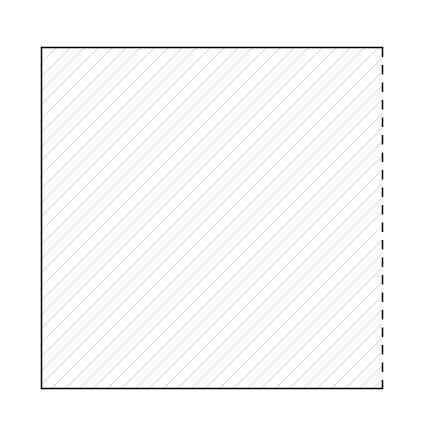
\includegraphics{fig1.png}
		\caption{L'insieme contiene solo tre lati del quadrato}
		\label{fig:fig1}
	\end{centering}
\end{figure}

\begin{prop}{Unione finita di chiusi}{unioneChiusi}
	Unione finita di chiusi è un insieme chiuso.
\end{prop}

\begin{proof}
	Siano \(C_1,\dots,C_n\) sottoinsiemi chiusi di \(X\), dobbiamo dimostrare che il complementare dell'unione è un aperto:
	\[
		\setc{\left(\bigcup_{i=1}^n C_i\right)}=\bigcap_{i=1}^n\setc{C_i},
	\]
	che è aperto in quanto per le proprietà dello spazio topologico.
\end{proof}

\begin{prop}{Intersezione qualsiasi di chiusi}{intersezioneChiusi}
	Intersezione qualsiasi di chiusi è un insieme chiuso.
\end{prop}

\begin{proof}
	Analoga alla precedente.
\end{proof}
%%%%%%%%%%%%%%%%%%%%%%%%%%%%%%%%%%%%%%%%%%%
%
%LEZIONE 02/03/2016 - SECONDA SETTIMANA (2)
%
%%%%%%%%%%%%%%%%%%%%%%%%%%%%%%%%%%%%%%%%%%%
\begin{ese}
	Su \(\R\) con la topologia euclidea, gli intervalli \([a,b],[a,+\infty)\) e \((-\infty,b]\), sono insiemi chiusi.
\end{ese}

\begin{ese}
	In uno spazio metrico \((X,d)\), i dischi chiusi
	\[
		\overline{D_r(x)}=\Set{d(y,x)\le r},
	\]
	sono insiemi chiusi.
\end{ese}

\begin{ese}
	Ogni sottoinsieme è chiuso in un insieme con la topologia discreta.
\end{ese}

\begin{defn}{Applicazione chiusa}{applChiusa}\index{Applicazione!chiusa}
	Un'applicazione \(f\colon X\to Y\) tra spazi topologici si dice \emph{chiusa} se manda chiusi in chiusi, ovvero
	\[
		\setc{f(A)}\in \Tau_Y,\,\fa \setc{A}\in \Tau_X.
	\]
\end{defn}

\begin{oss}
	Un'applicazione \(f\colon X\to Y\) tra spazi topologici è continua se e soltanto se la controimmagine di un chiuso è un chiuso
\end{oss}

\begin{oss}
	Un'applicazione \(f\colon X\to Y\) tra spazi topologici, continua e biiettiva, è un omeomorfismo, se e soltanto se \(f\) è chiusa.
\end{oss}
%%%%%%%%%%%%%%%%%%%%%%%%%%%%%%
%INTERIORI, ESTERIORI E BORDI%
%%%%%%%%%%%%%%%%%%%%%%%%%%%%%%
\section{Interiori, esteriori e bordi}
Con \(X\) faremo sempre riferimento ad un insieme dotato di una topologia \(T\)

\begin{defn}{Chiusura di un insieme}{chiusura}\index{Chiusura}
	Sia \(B\) un sottoinsieme qualsiasi di \(X\).
	Si definisce \emph{chiusura} di \(B\), l'intersezione di tutti i chiusi che contengono \(X\), ovvero
	\[
		\overline{B}=\bigcap\Set{C\subset X | B\subset C\text,C\text{chiuso}}.
	\]
\end{defn}

\begin{oss}
	\(\overline{B}\) è il più piccolo chiuso che contiene \(B\).
\end{oss}

\begin{defn}{Interiore di un insieme}{interiore}\index{Interiore}
	Sia \(B\) un sottoinsieme qualsiasi di \(B\).
	Si definisce \emph{interiore} di \(B\), l'insieme di tutti gli aperti contenuti in \(B\), ovvero
	\[
		\mathring{B}=\bigcup\Set{A\subset X | A\subset B,A\text{ aperto}}.
	\]
\end{defn}

\begin{oss}
	\(\mathring{B}\) è il più grande aperto contenuto in \(B\).
\end{oss}

\begin{oss}
	In generale vale
	\[
		\mathring{B}\subseteq B\subseteq \overline{B},
	\]
	dove l'uguaglianza vale se \(B\) è aperto nel primo caso e se \(B\) è chiuso nel secondo.
\end{oss}

\begin{defn}{Esteriore di un insieme}{esteriore}\index{Esteriore}
	Sia \(B\) un sottoinsieme qualsiasi di \(B\).
	Si definisce \emph{esteriore} di \(B\) il complementare della sua chiusura, ovvero
	\[
		\ext B=\setc{\overline{B}}=X\setminus \overline{B}.
	\]
\end{defn}

\begin{oss}
	Per definizione, l'esteriore di un insieme è sempre aperto.
\end{oss}

\begin{defn}{Bordo di un insieme}{bordo}\index{Bordo}
	Sia \(B\) un sottoinsieme qualsiasi di \(B\).
	Si definisce \emph{bordo} di \(B\) il complementare dell'unione digiunta dell'interiore e dell'esteriore di \(B\), ovvero
	\[
		\pd B=\setc{\{\mathring{B}\sqcup \ext B\}}=X\setminus\{\mathring{B}\cup\ext B\}.
	\]
\end{defn}

\begin{oss}
	Dal momento che l'interiore e l'eseteriore di \(B\) sono entrambi aperti, si avrà che \(\pd B\) è chiuso.
\end{oss}

\begin{oss}
	La figura \ref{fig:fig2} mostra un esempio di sottoinsieme di \(\R^2\) e la sua suddivisione.
\end{oss}

\begin{figure}[tp]
	\begin{centering}
		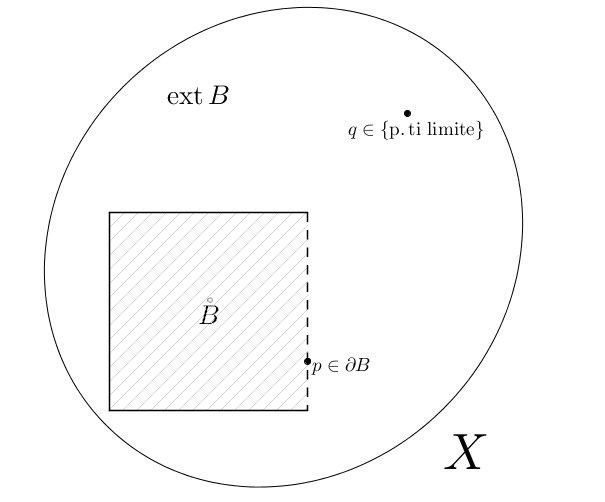
\includegraphics{fig2.png}
		\caption{Un generico insieme in \(\R^2\).}
		\label{fig:fig2}
	\end{centering}
\end{figure}

\begin{lem}\label{lem:intEst1}
	Sia \(B\) un sottoinsieme di \(X\), allora
	\[
		X=\mathring{B}\sqcup \pd B\sqcup \ext B.
	\]
\end{lem}

\begin{proof}
	Segue immediatamente dalla definizione di \(\pd B\).
\end{proof}

\begin{lem}\label{lem:intEst2}
	Sia \(B\) un sottoinsieme di \(X\), allora
	\[
		p\in \mathring{B} \iff \ex U_p\in T:U_p\subseteq B.
	\]
\end{lem}

\begin{proof}
	Dal momento che \(\mathring{B}\) è definito come l'unione degli aperti contenuti in \(B\) si ottiene facilmente la tesi.
\end{proof}

\begin{lem}\label{lem:intEst3}
	Sia \(B\) un sottoinsieme di \(X\), allora
	\[
		p\in \ext B\iff \ex U_p\in T:U_p\cap B=\emptyset.
	\]
\end{lem}

\begin{proof}
	Dal momento che \(\ext B\) è definito come il complementare della chiusura di \(B\), avremo che, se \(p\in \ext B\),
	\[
		\begin{split}
			p\in \setc{\overline{B}} & \iff p\in \setc{\left(\bigcap_{\substack{C\text{ chiuso}\\C\supset B}}C\right)}\\
			& \iff p\in \bigcup_{\substack{C\text{ chiuso}\\C\supset B}}\setc{C}\\
			& \iff p\in \setc{C},
		\end{split}
	\]
	dove \(C\) è chiuso e contiene \(B\), che implica \(\setc{C}\) è aperto e disgiunto da \(B\).
	Quindi
	\[
		p\in \setc{C}\in T,\setc{C}\cap B=\emptyset.
	\]
	Il viceversa si mostra in modo analogo.
\end{proof}

\begin{lem}\label{lem:intEst4}
	Sia \(B\) un sottoinsieme di \(X\), allora
	\[
		p\in\pd B \iff \fa U_p\in T\implies U_p\cap B\neq\emptyset,U_p\cap \setc{B}\neq\emptyset.
	\]
\end{lem}

\begin{proof}
	Segue dai due lemmi precedenti.
\end{proof}

\begin{lem}\label{lem:intEst5}
	Sia \(B\) un sottoinsieme di \(X\), allora
	\[
		B\text{ aperto }\iff B=\mathring{B}.
	\]
\end{lem}

\begin{proof}
	Segue dal lemma \ref{lem:intEst2}.
\end{proof}

\begin{lem}\label{lem:intEst6}
	Sia \(B\) un sottoinsieme di \(X\), allora
	\[
		B\text{ chiuso }\iff B=\overline{B}\iff\pd B\subset B.
	\]
\end{lem}

\begin{proof}
	La prima implicazione segue banalmente dalla definizione.
	Osserviamo che
	\[
		\pd B=\setc{\{\mathring{B}\cup\ext B\}}=\setc{\mathring{B}}\cap\setc{\ext B},
	\]
	ma \(\ext B=\setc{\overline{B}}\), per cui \(\setc{\ext B}=\overline{B}\).
	Quindi
	\[
		\pd B=\setc{\mathring{B}}\cap \overline{B}=\setc{\mathring{B}}\cap B\subset B,
	\]
	in quanto \(\mathring{B}\subset B\).
	Il viceversa è analogo.
\end{proof}

\begin{defn}{Punto limite}{puntoLimite}\index{Punto limite}
	Sia \(B\) un sottoinsieme qualsiasi di \(X\).
	Un punto \(q\in X\), si dice \emph{punto limite}, o di \emph{accomulazione}, per \(B\), se ogni intorno di \(U_q\) contiene un punto di \(B\) distinto da \(q\).
\end{defn}

\begin{oss}
	In generale, preso un sottoinsieme \(B\subset X\), si ha che il bordo di \(B\) è distinto dall'insieme dei suoi punti limite.
	Infatti, se consideriamo
	\[
		\mathcal{R}=\Set{(x,y)\in\R^2 | 1\le x<3,2\le y\le 4},
	\]
	mostrato sempre in figura \ref{fig:fig1}, ed il punto \(q=(6,7)\), possiamo definire il sottoinsieme
	\[
		B=\mathcal{R}\cup\{q\}.
	\]
	In questo caso avremo che il bordo di \(B\) è costituito dai lati di \(\mathcal{R}\) e il punto \(q\).
	D'altronde, l'insieme dei punti limite di \(B\) sarà la chiusura di \(\mathcal{R}\).
\end{oss}

\begin{ese}
	Prendiamo \(X=\R\).
	Avremo che l'insieme dei punti limite di \(\Z\) è vuoto.
	Mentre l'insieme dei punti limite di \(\{\frac{1}{n}\}_{n\in\N}\) sarà \(\{0\}\), che non è un elemento dell'insieme.
\end{ese}

\begin{defn}{Sottoinsieme denso}{denso}\index{Sottoinsieme denso}
	Sia \(B\) un sottoinsieme qualsiasi di \(X\).
	\(B\) si dice \emph{denso} in \(X\) se la sua chiusura coincide con \(X\).
\end{defn}

\begin{pr}
	Sia \(B\) un sottoinsieme di \(X\), allora
	\[
		B\subset X\text{ è denso }\iff\fa x \in X\,\ex x_n \in B : x_n \to x.
	\]
\end{pr}

\begin{pr}
	Sia \(B\) un sottoinsieme di \(X\), allora
	\[
		B\subset X\text{ è denso }\iff A\cap B\neq\emptyset,\,\fa A\in T.
	\]
\end{pr}

\begin{ese}
	\(\Q\) è un sottoinsieme denso in \(\R\) con la topologia euclidea.
\end{ese}

\begin{ese}
	\(\Q^n\) è un sottoinsieme denso in \(\R^n\) con la topologia euclidea.
\end{ese}

\begin{oss}
	Vedremo in seguito che sia \(\Q\) che \(\Q^n\) sono numerabili.
\end{oss}
%%%%%%%%%%%%%%%%%%%%%%
%VARIETA' TOPOLOGICHE%
%%%%%%%%%%%%%%%%%%%%%%
\section{Varietà topologiche}

\begin{defn}{Spazio localmente euclideo}{spazioLocEuclideo}\index{Spazio!localmente euclideo}
	Uno spazio topologico \(X\) si definisce \emph{localmente euclideo} di dimensione \(n\), se ogni punto \(p\in X\), possiede un intorno \(U_p\) tale che \(U_p\) è omeomorfo ad un aperto di \(\R^n\).
\end{defn}

\begin{oss}
	In generale questa definizione implica che ogni intorno \(U_p\) è omeomorfo a tutto \(\R^n\), infatti \(U_p\) è omeomorfo ad un disco \(D_r(x)\) di \(\R^n\), ma
	\[
		D_r(x)\approx D_1(\bar{x})\approx \R^n.
	\]
\end{oss}

\begin{defn}{Spazio di Hausdorff}{spazioHausdorff}\index{Spazio!di Hausdorff}
	Uno spazio topologico \(X\) si dice \emph{di Hausdorff}, o \(T2\), se
	\[
		\fa p,q\in X,\,\ex U_p,U_q:U_p\cap U_q=\emptyset.
	\]
\end{defn}

\begin{oss}
	Uno spazio di Hausdorff, che si dice anche spazio separato, ci dice che esistono abbastanza aperti affinchè ogni punto sia separato dagli altri.
\end{oss}

\begin{oss}
	Ogni spazio metrico è di Hausdorff, infatti, presi \(x,y\in X\), se fissiamo \(d=d(x,y)\), avremo
	\[
		B_{\frac{d}{2}}(x)\cap B_{\frac{d}{2}}(y)=\emptyset.
	\]
\end{oss}

\begin{ese}
	Sia \(X=\{1,2,3\}\) su cui definiamo la topologia \(T=\{\emptyset,X,\{1\},\{2,3\}\}\).
	Lo spazio topologico \((X,T)\) non è di Hausdorff, infatti ogni intorno di \(2\) contiene anche \(3\).
\end{ese}

\begin{prop}{Proprietà degli spazi di Hausdorff}{propSpaziHausdorff}
	Sia \(X\) uno spazio di Hausdorff, allora
	\begin{itemize}
		\item Ogni punto \(p\) costituisce un sottoinsieme chiuso.
		\item Se \(\{x_n\}_{n\in \N}\) è una successione convergente, allora
		      \[
			      \lim_{n\to +\infty}x_n=x,
		      \]
		      è unico.
	\end{itemize}
\end{prop}

\begin{proof}
	\begin{itemize}
		\item Sia \(p\in X\), vogliamo mostrare che \(\setc{\{p\}}\) è aperto, ma
		      \[
			      \setc{\{p\}}=X\setminus\{p\}\implies q\in \setc{\{p\}},\,\fa q\neq p,
		      \]
		      quindi, per la definizione di spazio di Hausdorff, esisterà un intorno \(U_q\) tale che \(p\notin U_q\), ovvero
		      \[
			      \setc{\{p\}}=\setc{\{\mathring{p}\}},
		      \]
		      per cui \(\setc{\{p\}}\) è aperto.
		\item Supponiamo per assurdo che esistano \(x,y\) tali che
		      \[
			      \lim_{n\to +\infty}x_n=x\neq y=\lim_{n\to +\infty}x_n,
		      \]
		      per Hausdorff avremo che esistono due intorni \(U_x,U_y\) tali che
		      \[
			      U_x\cap U_y=\emptyset,
		      \]
		      ma ciò è assurdo in quanto
		      \[
			      x_n\to x\implies \ex N>0:x_n\in U_y,\,\fa n>N,
		      \]
		      ma
		      \[
			      x_n\to x\implies \ex N'>0:x_n\in U_x,\,\fa n>N',
		      \]
		      ovvero
		      \[
			      U_x\cap U_y\neq \emptyset.
		      \]
	\end{itemize}
\end{proof}

\begin{defn}{Varietà topologica}{varietàTopologica}\index{Varietà topologica}
	Uno spazio topologico \((M,T)\) si dice \emph{varietà topologica} di dimensione \(n\), se soddisfa
	\begin{enumerate}
		\item \((M,T)\) è localmente euclideo di dimensione \(n\).
		\item \((M,T)\) è uno spazio di Hausdorff.
		\item \((M,T)\) ammette una base numerabile \(\mathcal{B}=\{B_n\}_{n\in \N}\).
	\end{enumerate}
\end{defn}

\begin{ese}
	\(\R^n\) rispetto alla topologia standard è una varietà topologica, infatti
	\begin{enumerate}
		\item Banalmente verificato.
		\item Vero poichè con la topologia standard \(\R^n\) è uno spazio metrico.
		\item Basta prendere \(\mathcal{B}=\{B_r(\bar{q})\}_{\Q^{n+1}}\), con \(\bar{q}=(q_1,\dots,q_n)\in\Q^n\) e \(r\in \Q\).
	\end{enumerate}
\end{ese}
%%%%%%%%%%%%%%%%%%%%%%%%%%%%%%%%%%%%%%%%%
%
%LEZIONE 07/03/2016 - TERZA SETTIMANA (1)
%
%%%%%%%%%%%%%%%%%%%%%%%%%%%%%%%%%%%%%%%%%
\begin{notz}
	Da questo momento potremmo utilizzare la seguente notazione:
	\begin{itemize}
		\item \(T_2\) per gli spazi di Hausdorff, per indicare la validità del secondo assioma di separazione.
		\item \(N_2\) per gli spazi a base numerabile, per indicare la validità del secondo assioma di numerabilità.
	\end{itemize}
\end{notz}

\begin{defn}{Ricoprimento aperto}{ricoprimentoAperto}\index{Ricoprimento aperto}
	Sia \(X\) uno spazio topologico.
	Si definisce \emph{ricoprimento aperto} di \(X\) una famiglia di aperti \(\mathcal{A}=\{A_i\}_{i\in I}\) tale che
	\[
		X=\bigcup_{i\in I}A_i.
	\]
\end{defn}

\begin{ese}
	In \(\R^2\) le palle di centro l'origine e raggio \(n\in\N\) sono un ricoprimento di \(\R^2\), infatti
	\[
		\bigcup_{n\in\N}D_n(\bar{0})=\R^2.
	\]
\end{ese}

\begin{prop}{Ricoprimenti aperti per spazi \(N_2\)}{ricoprimentiApertiN2}
	Sia \(X\) uno spazio topologico a base numerabile.
	Allora ogni ricoprimento aperto di \(X\) ammette un sottoricoprimento numerabile.
\end{prop}

\begin{proof}
	Sia \(\mathcal{A}=\{A_i\}_{i\in I}\) un arbitrario ricoprimento aperto di \(X\).\graffito{ovvero \(I\) non è necessariamente numerabile}
	Sia \(\mathcal{B}\) una base numerabile di \(X\), quindi
	\[
		\fa A_i\,\ex B'_i\in\mathcal{B}:B'_i\subseteq A_i,
	\]
	quindi
	\[
		\mathcal{B}=\{B_j\}_{j\in\N}.
	\]
	Consideriamo ora il sottoricoprimento \(\mathcal{A}'=\{B'_i\}_{i\in I'}\) con \(I'\subset\N\) numerabile.
	Resta quindi da mostrare che \(\mathcal{A}'\) costituisce effettivamente un ricoprimento, ovvero che
	\[
		X=\bigcup_{i\in I'}B'_i.
	\]
	Ora, dal momento che \(\mathcal{A}\) costituisce un ricoprimento, preso un qualsiasi \(x_i\in X\), esisterà \(A_{i_0}\in \mathcal{A}\) tale che \(x\in A_{i_0}\).
	Ma \(\mathcal{B}\) è una base, per cui \(A_{i_0}\) è unione di elementi di \(\mathcal{B}\), ovvero
	\[
		\ex B'_{i_0}:x\in B'_{i_0}.\qedhere
	\]
\end{proof}

\begin{prop}{\(\R^n\) è a base numerabile}{RnBaseNumerabile}
	Consideriamo \(\R^n\) dotato della topologia euclidea.
	Allora \(\R^n\) è a base numerabile.
\end{prop}

\begin{proof}
	Preso \(x\in\R^n\) e comunque preso un intorno \(A_x\) di \(x\), esisterà un disco centrato in \(x\) di raggio \(r\in\Q\) contenuto in \(A_x\).
	Questo è vero poichè posso approssimare ogni reale con una successione di razionali, cioè i dischi aperti di raggio razionale costituiscono una base numerabile per gli intorni di \(x\in\R^n\).\graffito{si riferisce al primo assioma di numerabilità \(N_1\)}

	Per ottenere una base numerabile di tutto \(\R^n\), ovvero che soddisfi \(N_2\), basta considerare i dischi aperti \(D_r(\bar{q})\), dove \(\bar{q}\in\Q^n\subset\R^n\) e \(r\in\Q\), ovvero la famiglia
	\[
		\{D_r(\bar{q})\}_{(r,\bar{q})\in\Q^{n+1}},
	\]
	che è proprio un ricoprimento aperto e numerabile di \(\R^n\) poichè
	\[
		\fa x\in\R^n\,\ex\bar{q}_k\to x.
	\]
	Ed è pertanto una base per la caratterizzazione \ref{pr:caratBasi}.
\end{proof}

\begin{oss}
	Ogni spazio metrico \((X,d)\) soddisfa il primo assioma di numerabilità \(N_1\).
\end{oss}

\begin{oss}
	Ogni spazio metrico \((X,d)\) è a base numerabile se e soltanto se contiene un sottoinsieme denso numerabile.
\end{oss}
%!TEX root = ../main.tex
%%%%%%%%%%%%%%%%%%%%%%%%%%%%%%%%%%%%%%%%%
%
%LEZIONE 07/03/2016 - TERZA SETTIMANA (1)
%
%%%%%%%%%%%%%%%%%%%%%%%%%%%%%%%%%%%%%%%%%
\chapter{Nuovi spazi topologici}
%%%%%%%%%%%%
%SOTTOSPAZI%
%%%%%%%%%%%%
\section{Sottospazi}

\begin{defn}{Topologia indotta}{topologiaIndotta}\index{Topologia!indotta}
	Sia \(X\) uno spazio topologico e sia \(B\) un sottoinsieme qualsiasi di \(X\).
	La \emph{topologia indotta} su \(B\) dalla topologia su \(X\) è la seguente:
	\[
		U\text{ aperto di }B\iff\,\ex V\text{ aperto di } X:U=B\cap V.
	\]
\end{defn}

\begin{defn}{Sottospazio topologico}{sottospazio}\index{Sottospazio topologico}
	Sia \(X\) uno spazio topologico e sia \(B\) un sottoinsieme qualsiasi di \(X\).
	\(B\) si definisce \emph{sottospazio} di \(X\) se dotato della topologia indotta.
\end{defn}

\begin{oss}
	Un sottospazio è banalmente uno spazio topologico, infatti
	\begin{itemize}
		\item Se \(U_1,U_2\) sono aperti di \(B\) avremo che \(U_1=B\cap V_1,U_2=B\cap V_2\), dove \(V_1,V_2\) sono aperti di \(X\), per cui
		      \[
			      U_1\cup U_2=(B\cap V_1)\cup(B\cap V_2)=B\cap(V_1\cup V_2),
		      \]
		      dove \(V_1\cup V_2\) è un aperto di \(X\) in quanto unione di aperti.
		      Per cui dalla definizione \(U_1\cap U_2\) è un aperto di \(B\).
		\item Analogamente a prima avremo
		      \[
			      U_1\cap U_2=(B\cap V_1)\cap (B\cap V_2)=B\cap(V_1\cap V_2),
		      \]
		      dove \(V_1\cap V_2\) è un aperto di \(X\) in quanto intersezione di aperti.
		\item Ovviamente \(B\) e \(\emptyset\) sono aperti di \(B\) in quanto
		      \[
			      B=B\cap X,
		      \]
		      dove \(X\) è ovviamente aperto, e
		      \[
			      \emptyset=B\cap \emptyset.
		      \]
	\end{itemize}
\end{oss}

\begin{oss}
	Sia \((X,d)\) uno spazio metrico dotato della topologia indotta da \(d\) e sia \(B\) un sottoinsieme di \(X\).
	Avremo che la distanza ristretta \(d_B\colon B\times B\to\R^{\ge 0}\) definisce una distanza su \(d\).
	Allora \((B,d_B)\) è omeomorfo a \(B\) dotato della topologia di sottospazio.
\end{oss}

\begin{ese}
	Consideriamo il sottoinsieme \(B=[-1,2]\cup(3,4)\subset\R\).
	Si dimostri che \([-1,2]\) è aperto di \(B\), dotato della topologia di sottospazio.
\end{ese}

\begin{sol}
	Per definizione dobbiamo scrivere \([-1,2]\) come intersezione di \(B\) e un aperto di \(\R\), quindi basta scrivere
	\[
		[-1,2]=B\cap(-2,3),
	\]
	dove \(-2,3\) è ovviamente un aperto di \(\R\).
\end{sol}

\begin{ese}
	In \(\R\) si consideri la successione convergente \(C=\left\{\frac{1}{n}\right\}_{n\in\N}\).
	Consideriamo \(C\) come sottospazio di \(\R\), si dica se:
	\begin{itemize}
		\item \(C\) è uno spazio topologico discreto.
		\item L'origine è un elemento di \(C\).
	\end{itemize}
\end{ese}

\begin{sol}
	\begin{itemize}
		\item Un generico elemento di \(C\) è del tipo \(\frac{1}{n}\), mi basta quindi dimostrare che esiste un aperto in \(C\) che contiene solamente \(\frac{1}{n}\).
		      Mi basta quindi
		      \[
			      \left\{\frac{1}{n}\right\}=\left(\frac{1}{n}-\e,\frac{1}{n}+\e\right)\cap C,
		      \]
		      dove \(\e\) è un valore sufficientemente piccolo, in particolare
		      \[
			      \e<d\left(\frac{1}{n},\frac{1}{n+1}\right)=\frac{1}{n(n+1)}<\frac{1}{n}.
		      \]
		\item No, poichè \(0\neq \frac{1}{n},\,\fa n\in\N\).
	\end{itemize}
\end{sol}

\begin{ese}
	Consideriamo l'applicazione
	\[
		\exp\colon [0,2\p)\to S^1\subset \R^2\approx \C,\q\mapsto e^{i\,\q}=(\cos\q,\sin\q).
	\]
	Si dica se \(\exp\) costituisce un omeomorfismo.
\end{ese}

\begin{sol}
	Per l'analisi sappiamo che \(\exp\) è continua, inoltre risulta iniettiva su \([0,2\p)\) in quanto funzione periodica di periodo pari proprio a \(2\p\).
	Infine \(\exp\) è banalmente suriettiva su \(S^1\).

	Resterebbe da verificare se è aperta nelle topologie di sottospazi \([0,2\p)\subset\R,S^1\subset\R^2\).
	Ma si mostra facilmente che non lo è, infatti, consideriamo \([0,\p/2)\) che è aperto in \([0,2\p)\) in quanto \([0,\p/2)=[0,2\p)\cap(-1,\p/2)\).
	Avremo che l'immagine \(\exp([0,\p/2))\) non è aperta in \(S^1\) in quanto il punto \((1,0)\) non appartiene all'interiore di \(S^1\).
\end{sol}

\begin{defn}{Embedding topologico}{embedding}\index{Embedding}
	Sia \(X\) uno spazio topologico e sia \(A\) un sottoinsieme di \(X\).
	Un \emph{embedding} topologico è un'applicazione continua e iniettiva
	\[
		f\colon A\hookrightarrow X,
	\]
	che è omeomorfismo sull'immagine \(f(A)\).
\end{defn}

\begin{oss}
	Un'applicazione iniettiva è ovviamente biiettiva sull'immagine.
\end{oss}

\begin{teor}{Proprietà universale della topologia di sottospazi}{propUniversaleSottospazi}
	Sia \(B\subset X\) un sottospazio topologico.
	Sia \(Y\) uno spazio topologico qualsiasi.
	Allora
	\[
		f\colon Y\to B,
	\]
	è continua se e soltanto se la composizione
	\[
		Y\overset{f}{\to}B\overset{i}{\hookrightarrow}X,
	\]
	è continua.
\end{teor}

\begin{proof}
	\(f\) è continua se e soltanto se \(f^{-1}(U)\) è aperto in \(Y\) per ogni \(U\) aperto di \(B\).
	Ma \(U\) è aperto in \(B\) se e solo se, per definizione, \(U=B\cap V\), dove \(V\) è un aperto di \(X\).
	Quindi
	\[
		U=i^{-1}(V)\implies f^{-1}(U)=\big(i\circ f\big)^{-1}(V),
	\]
	ovvero \(f^{-1}(U)\) è un aperto di \(Y\) se e solo se \(i\circ f\) è continua
\end{proof}

\begin{oss}
	La topologia di sottospazio è l'unica che soddisfa questa proprietà universale.%TODO
\end{oss}
%%%%%%%%%%%%%%%%%%%%%%%%%%%%%%%%%%%%%%%%%
%
%LEZIONE 09/03/2016 - TERZA SETTIMANA (2)
%
%%%%%%%%%%%%%%%%%%%%%%%%%%%%%%%%%%%%%%%%%
Preso \(B\subset X\) un sottospazio topologico di \(X\), valgono le seguenti proprietà:

\begin{pr}\label{ssp:1}
	L'inclusione
	\[
		i\colon B\hookrightarrow X,
	\]
	è un embedding.
\end{pr}

\begin{pr}\label{ssp:2}
	Se \(f\colon X\to Y\) è continua, allora la restrizione
	\[
		f|_B\colon B\to Y,
	\]
	è continua.
\end{pr}

\begin{pr}\label{ssp:3}
	Se \(f\colon X\to Y\) è continua, allora la restrizione sull'immagine
	\[
		f|_B\colon B\to f(B),
	\]
	è continua e suriettiva.
\end{pr}

\begin{pr}\label{ssp:4}
	I chiusi di \(B\) sono precisamente le intersezioni con i chiusi di \(X\).
\end{pr}

\begin{pr}\label{ssp:5}
	Se \(\mathcal{B}\) è una base di \(X\), allora
	\[
		\mathcal{B}_B=\Set{B\cap U:U\in\mathcal{B}},
	\]
	è base di \(B\).
\end{pr}

\begin{pr}\label{ssp:6}
	Se \(X\) è uno spazio di Hausdorff, allora lo è anche \(B\).
\end{pr}

\begin{pr}\label{ssp:7}
	Se \(X\) è a base numerabile, allora lo è anche \(B\).
\end{pr}

\begin{prop}{Grafico omeomorfo al dominio dell'applicazione}{graficoOmeoDominio}
	Presa un'applicazione continua \(f\colon U\to\R^k,U\) aperto di \(\R^n\).
	Allora il grafico
	\[
		\Gamma_f=\Set{(x,y)\in\R^n\times\R^k | x\in U,y=f(x)\in\R^k},
	\]
	è un sottospazio di \(R^{n+k}\) omeomorfo a \(U\) aperto di \(\R^n\).
\end{prop}

\begin{proof}
	Per la proprietà \ref{ssp:3} l'applicazione \(\j_f\colon U\to\Gamma_f\) è continua e suriettiva.
	D'altronde \(\j_f\) è anche iniettiva, in quanto mappa \(x\mapsto \big(x,y=f(x)\big)\), con inversa
	\[
		\j_f^{-1}\colon \Gamma_f\to U,(x,y)\mapsto x,
	\]
	che è continua in quanto restrizione dell'applicazione continua
	\[
		\R^{n+k}\to\R^n,(x,y)\mapsto x.\qedhere
	\]
\end{proof}

\begin{ese}
	Si dimostri che
	\[
		V=\Set{(x,y)\in\R^2 | y=\abs{x}},
	\]
	è omeomorfo a \(\R\).
\end{ese}

\begin{sol}
	Per definizione avremo \(V=\Gamma_{\abs{x}}\), dove
	\[
		\abs{x}\colon\R\to\R, x\mapsto \begin{cases}
			x  & x\ge 0 \\
			-x & x<0
		\end{cases}
	\]
	per la proposizione precedente \(V\) è omeomorfo al dominio di \(\abs{x}\) che nel nostro caso \(\R\).
	Quindi
	\[
		V\approx \R.
	\]
\end{sol}

\begin{exe}[per casa]
	Si dimostri che un aperto di \(\R^n\) è omeomorfo ad una varietà topologica \(T_f\) di dimensione \(n\).
\end{exe}

\begin{oss}
	Quindi uno spazio topologico che è localmente il grafico di una funzione continua, è localmente euclideo.
\end{oss}

\begin{prop}{Sfere come varietà topologiche}{sferaVarietaTop}
	La sfera unitaria di dimensione \(n\)
	\[
		S^n=\Set{x\in\R^{n+1} | \norma{x}^2=1},
	\]
	è una varietà topologica di dimensione \(n\).
\end{prop}

\begin{proof}
	Dal momento che \(\R^{n+1}\) è uno spazio di Hausdorff a base numerabile, per le proprietà \ref{ssp:6} e \ref{ssp:7}, lo è anche \(S^n\).
	Per concludere resta da dimostrare che \(S^n\) è localmente euclideo, ma ciò segue dal fatto che \(S^n\) è localmente il grafico di un'applicazione \(U\subset\R^n\to S^n\).
	Infatti, per definizione \(x=(x_1,\ldots,x_{n+1})\in S^n\) quando \(\norma{x}^2=1\), per cui
	\[
		\ex i\in\Set{1,\ldots,n+1}:x_i\neq 0,
	\]
	ovvero
	\[
		x_i=\sqrt{1-x_1^2- \ldots -\hat{x}_i^2- \ldots -x_{n+1}^2}=f(x_1,\ldots,\hat{x}_i^2,\ldots x_{n+1}),
	\]
	che è una funzione continua \(f\colon\R^n\to \R\).
	Per cui, in un intorno di \(x\in S^n\), avremo che \(S^n\) è il grafico di \(f\).
	Ovvero \(S^n\) è è localmente euclideo essendo localmente omeomorfo ad \(\R^n\) per la proposizione \ref{pr:graficoOmeoDominio}.
\end{proof}

\begin{ese}
	Si dimostri che
	\[
		S^1=\Set{(x,y)\in\R^2 | x^2+y^2=1},
	\]
	è una varietà topologica di dimensione \(1\).
\end{ese}

\begin{sol}
	Ripercorriamo la dimostrazione della proposizione precedente:
	\(S^1\) è di Hausdorff e a base numerabile in quanto lo è \(\R^2\).
	Inoltre è localmente euclideo, ovvero esiste un ricoprimento aperto \(\mathcal{A}=\Set{A}_{i\in I}\) tale che
	\[
		S^1=\bigcup_{i\in I}A_i \qquad\text{e}\qquad A_i\approx \R.
	\]
	Questo poichè, nel semicerchio superiore \(A_1\), \(S^1\) è il grafico di \(y=\sqrt{1-x^2}\) che è omeomorfo al dominio \((-1,1)\).
	Analogamente, nel semicerchio inferiore \(A_2\), \(S^1\) è il grafico di \(y=-\sqrt{1-x^2}\).

	Per includere in punti con \(y=0\) ci basta considerare il semicerchio destro \(A_3\) e sinistro \(A_4\), rispettivamente grafici di
	\[
		x=\sqrt{1-y^2}\qquad\text{e}\qquad x=-\sqrt{1-y^2}.
	\]
	Avremo quindi \(S^1=A_1\cup A_2\cup A_3\cup A_4\), pertanto \(S^1\) è localmente euclideo in quanto
	\[
		A_i\approx (-1,1)\approx \R.
	\]
\end{sol}

\begin{prop}{Funzioni definite a tratti}{funzioniATratti}
	Sia \(X\) uno spazio topologico che può essere scritto come unione finita di insiemi chiusi
	\[
		X=C_1 \cup \ldots \cup C_k.
	\]
	Allora, comunque preso \(i\), esiste un'applicazione continua \(f_i\colon C_i\to Y\) tale che
	\[
		f_i|_{C_i \cap C_j}=f_j|_{C_i \cap C_j},
	\]
	se e soltanto se esiste un'unica funzione continua \(f\colon X\to Y\), tale che
	\[
		f|_{C_i}=f_i.
	\]
\end{prop}

\begin{ese}
	Su \(\R=(-\infty,0]\cup [0,+\infty)\), consideriamo ad esempio
	\[
		\abs{x}\colon\R\to\R^+,x\mapsto \begin{cases}
			x  & x \ge 0 \\
			-x & x < 0
		\end{cases}
	\]
	avremo quindi
	\[
		f_1\colon(-\infty,0]\to \R^+,x\mapsto -x \qquad\text{e}\qquad f_2\colon [0,+\infty)\to\R^+,x\mapsto x,
	\]
	con \(f_1(0)=f_2(0)=0\) e
	\[
		f|_{(-\infty,0]}=f_1 \qquad \qquad f|_{[0,+\infty)}=f_2.
	\]
\end{ese}
%%%%%%%%%%%%%%%%
%SPAZI PRODOTTO%
%%%%%%%%%%%%%%%%
\section{Spazi prodotto}

\begin{defn}{Topologia prodotto}{topologiaProdotto}\index{Topologia!prodotto}
	Dati \(n\) spazi topologici \(X_1, \ldots, X_n\), la \emph{topologia prodotto} sul prodotto cartesiano
	\[
		X_1 \times \ldots \times X_n
	\]
	è definita dalla seguente base
	\[
		\mathcal{B}=\Set{(U_1 \times \ldots \times U_n) | U_i\in T_i,\,\fa i\in\Set{1, \ldots, n}}.
	\]
\end{defn}

\begin{oss}
	Naturalmente è sufficiente considerare tutte le combinazioni di aperti delle rispettive basi.
\end{oss}

\begin{ese}
	Consideriamo \(\R^2=\R \times \R\) con la topologia prodotto. La base di \(\R^2\) sarà dunque l'insieme di tutti i sottoinsiemi di \(\R^2\) che sono prodotto di aperti in \(\R\).
	Quindi, per la caratterizzazione degli aperti in \(\R\), tali sottoinsiemi saranno tutti i prodotti
	\[
		(a,b) \times (c,d),
	\]
	di intervalli aperti di \(\R\).
	Pertanto la base di \(\R^2\) è costituita dai rettangoli aperti, i quali avevamo osservato identificano la stessa base di \(\R^2\) definita dai dischi.
\end{ese}

\begin{defn}{Spazio prodotto}{spazioProdotto}\index{Spazio!prodotto}
	Dati \(n\) spazi topologici \(X_1, \ldots, X_n\), si definisce \emph{spazio prodotto}, il prodotto cartesiano
	\[
		X_1 \times \ldots \times X_n,
	\]
	con la topologia prodotto.
\end{defn}

\begin{prop}{Proiezioni di spazi prodotto sono continue}{proiezioniContinue}
	Sia \(X = X_1 \times \ldots \times X_n\) uno spazio prodotto.
	Allora le proiezioni
	\[
		\p_i \colon X \to X_i, (x_1, \ldots, x_i, \ldots, x_n)\mapsto x_i,
	\]
	sono tutte continue, suriettive e aperte.
\end{prop}

\begin{proof}
	Basta dimostrarlo per \(n=2\), infatti, se risultasse vero per \(X_1 \times X_2\) si potrebbe estendere ad \(X_1 \times X_2 \times X_3\) semplicemente ridefinendo \(Y_1 = X_1 \times X_2\), ovvero
	\[
		X_1 \times X_2 \times X_3 = (X_1 \times X_2) \times X_3 = Y_1 \times X_3.
	\]
	Dimostriamolo quindi per \(n=2\):
	\begin{itemize}
		\item La suriettività è vera per definizione.
		\item Preso \(U_1\) aperto di \(X_1\), avremo che
		      \[
			      \p_1^{-1}(U_1)=U_1 \times X_2,
		      \]
		      che è un aperto del prodotto in quanto \(X_2\) è per definizione un aperto di \(X_2\), mentre \(U_1\) è aperto di \(X_1\) per ipotesi.
		\item Per dimostrare che \(\p_i\) è aperto, è sufficiente mostrarlo per gli aperti della base, infatti
		      \[
			      \p_1(U_1 \times U_2) = U_1,
		      \]
		      che è aperto di \(X_1\), analogamente
		      \[
			      \p_2(U_1 \times U_2) = U_2,
		      \]
		      che è aperto di \(X_2\).\qedhere
	\end{itemize}
\end{proof}
%%%%%%%%%%%%%%%%%%%%%%%%%%%%%%%%%%%%%%%%%%
%
%LEZIONE 14/03/2016 - QUARTA SETTIMANA (1)
%
%%%%%%%%%%%%%%%%%%%%%%%%%%%%%%%%%%%%%%%%%%
\begin{teor}{Proprietà universale della topologia prodotto}{propUniversaleProdotto}
	Sia \(X_1 \times \ldots \times X_n\) un prodotto topologico e sia \(\p_i \colon X_1 \times \ldots \times X_n \to X_i\) la proiezione su ciascuna componente.
	Allora un'applicazione
	\[
		f \colon Y \to X_1 \times \ldots \times X_n,
	\]
	è continua se e soltanto se \(\p_i \circ f\) è continua \(\fa i=1,\ldots,n\).
\end{teor}

\begin{proof}
	Come abbiamo già osservato in precedenza, è sufficiente dimostrare una proposizione su spazi topologici nel caso \(n=2\).
	Consideriamo quindi il caso \(X\times Z\) con \(X=X_1\) e \(Z=X_2 \times \ldots \times X_n\).

	Per la continuità è sufficiente verificarla su una base, nel caso specifico della topologia prodotto su
	\[
		\mathcal{B} = \Set{U\times V | U\in T_X, V\in T_Z}.
	\]
	\graffito{\(\Leftarrow)\)}Per definizione \(f\) è continua se e soltanto se \(f^{-1}(U\times V)\) è aperta in \(Y\).
	Ma, per ipotesi,
	\[
		\big( \p_X \circ f \big)^{-1}(U) = f^{-1}\big( \p_X^{-1}(U) \big) = f^{-1}(U\times Z),
	\]
	è un aperto di \(Y\).
	Analogamente
	\[
		\big( \p_Z \circ f \big)^{-1}(V) = f^{-1}\big( \p_Z^{-1}(V) \big) = f^{-1}(X\times V),
	\]
	che è ancora un aperto di \(Y\).
	Osserviamo infine che
	\[
		f^{-1}(U\times V) = f^{-1}(U\times Z) \cap f^{-1}(X\times V),
	\]
	che è quindi aperta in quanto intersezione di aperti.

	\graffito{\(\Rightarrow)\)}Supponiamo che \(f\) sia continua, per cui ogni controimmagine di un elemento della base è aperto in \(Y\).
	Siano \(U,V\) rispettivamente aperti di \(X\) e \(Z\), avremo
	\begin{gather*}
		\big( \p_X \circ f \big)^{-1}(U) = f^{-1}\big( \p_X^{-1}(U) \big) = f^{-1}(U\times Z),\\
		\big( \p_Z \circ f \big)^{-1}(V) = f^{-1}\big( \p_Z^{-1}(V) \big) = f^{-1}(X\times V),
	\end{gather*}
	che sono entrambi aperti in \(Y\) in quanto controimmagini di elementi della base.
\end{proof}

\begin{cor}
	Un'applicazione
	\[
		F\colon \R^n\to\R^n, \bar{x}=(x_1,\ldots,x_n) \mapsto \big( f_1(\bar{x}),\ldots,f_n(\bar{x}) \big),
	\]
	è continua se e soltanto se ogni sua componente \(f_i\) è continua.
\end{cor}

\begin{proof}
	Segue banalmente dalla proprietà universale, infatti
	\[
		f_i = \p_i \circ f.\qedhere
	\]
\end{proof}

\begin{prop}{Unicità della topologia prodotto}{unicitàTopProdotto}
	Siano \(X_1,\ldots,X_n\) spazi topologici.
	Allora la topologia prodotto su \(X_1\times \ldots \times X_n\) è l'unica che soddisfa la proprietà universale.
\end{prop}

\begin{proof}
	%TODO P.64 PDF
\end{proof}

\begin{pr}\label{pr:prod1}
	La topologia prodotto è associativa, ovvero
	\[
		X \times Y \times Z \approx (X\times Y) \times Z \approx X\times (Y\times Z).
	\]
\end{pr}

\begin{pr}\label{pr:prod2}
	Comunque preso \(y_0\in Y\), l'inclusione
	\[
		i\colon X \hookrightarrow X\times Y, x\mapsto(x,y_0),
	\]
	è un embedding.
\end{pr}

\begin{pr}\label{pr:prod3}
	Se \(X,Y\) sono spazi di Hausdorff, allora
	\[
		X\times Y,
	\]
	è uno spazio di Hausdorff.
\end{pr}

\begin{pr}\label{pr:prod4}
	Se \(X,Y\) sono spazi a base numerabile, allora
	\[
		X\times Y,
	\]
	è uno spazio a base numerabile.
\end{pr}

\begin{prop}{Somma e prodotto di applicazioni continue}{sommaProdottoContinue}
	Siano \(f,g\colon X\to K\) applicazioni da uno spazio topologico in un gruppo (o campo) topologico, allora
	\[
		f+g \qquad\text{e}\qquad f\cdot g,
	\]
	sono applicazioni continue.
\end{prop}

\begin{proof}
	\(K\) è uno spazio topologico, quindi per la proprietà universale, \(f,g\colon X\to K\) sono continue se e soltanto se
	\[
		X \to K\times K, x\mapsto \big( f(x),g(x) \big),
	\]
	è continua.
	Inoltre
	\begin{gather*}
		+\colon K \times K \to K, (a,b) \mapsto a+b,\\
		\cdot \colon K\times K \to K, (a,b) \mapsto a\,b,
	\end{gather*}
	sono applicazione continue.
	Quindi \(f+g\) e \(f\cdot g\) sono continue in quanto composizione di applicazioni continue.
\end{proof}

\begin{prop}{Prodotto di varietà topologiche}{prodottoVarTopologiche}
	Siano \(M\) e \(N\) due varietà topologiche rispettivamente di dimensione \(m\) e \(n\).
	Allora \(M\times N\) è una varietà topologica di dimensione \(m+n\).
\end{prop}

\begin{proof}
	Per le proprietà \ref{pr:prod3} e \ref{pr:prod4} sappiamo che \(M\times N\) è uno spazio di Hausdorff a base numerabile.

	Resta da mostrare che è localmente omeomorfo ad \(\R^{m+n}\).
	Consideriamo quindi la base
	\[
		\mathcal{B} = \Set{U\times V | U\in M, V\in N},
	\]
	sappiamo, per definizione di varietà topologica, che \(U\approx \R^m\) e \(V\approx \R^n\), quindi
	\[
		U\times V \approx \R^m \times \R^n \approx \R^{m+n}.\qedhere
	\]
\end{proof}

\begin{ese}
	Dimostriamo che la ciambella, o toro, è omeomorfa al prodotto topologico di due cerchi.%TODO FIG

	Osserviamo che il toro corrisponde graficamente alla superficie di rotazione che si ottiene ruotando un cerchio di centro \((a,0)\) e raggio \(r<a\) attorno all'asse \(z\).

	Costruiamo quindi un esempio numerico prendendo un cerchio di raggio \(r=1\) e centro \((2,0)\).
	Avremo quindi le seguenti equazioni parametriche:
	\[
		(y-2)^2+z^2 = 1 : 	\begin{cases}
			x = 2+\cos\q \\
			y = \sin\q
		\end{cases}
	\]
	%TODO
\end{ese}
%%%%%%%%%%%%%%%%%
%SPAZI QUOZIENTE%
%%%%%%%%%%%%%%%%%
\section{Spazi quoziente}

\begin{defn}{Topologia quoziente}{topologiaQuoziente}\index{Topologia!quoziente}
	Sia \(\p\colon X \twoheadrightarrow Y\) un'applicazione suriettiva con \(X\) spazio topologico.
	Si definisce la \emph{topologia quoziente} su \(Y\) come segue:
	\[
		V \text{ è aperto in } Y \iff \p^{-1}(V) \text{ è aperto in }X.
	\]
\end{defn}

\begin{oss}
	La stessa definizione vale anche per i chiusi.
\end{oss}

\begin{defn}{Spazio quoziente}{spazioQuoziente}\index{Spazio!quoziente}
	Sia \(\p\colon X \twoheadrightarrow Y\) un'applicazione suriettiva con \(X\) spazio topologico.
	\(Y\) si definisce \emph{spazio quoziente} se dotato della topologia di sottospazio.
\end{defn}

\begin{notz}
	Per indicare che \(Y\) è uno spazio quoziente su \(X\) scriveremo
	\[
		Y = \frac{X}{\sim}
	\]
	Dove \(\sim\) indica la seguente relazione di equivalenza
	\[
		x_1 \sim x_2 \iff \p(x_1) = \p(x_2).
	\]
\end{notz}

\begin{defn}{Fibra di un punto}{fibra}\index{Fibra}
	Sia \(Y=X/\sim\) uno spazio quoziente e sia \(x_0\in Y\).
	Definiamo \emph{fibra} di \(x_0\) l'insieme di tutti i punti di \(X\) che hanno come immagine \(x_0\), ovvero
	\[
		\p^{-1}(x_0).
	\]
\end{defn}

\begin{oss}
	Per definizione, se \(x_1 \sim x_2\) diremo che \(x_1,x_2\) appartengono alla stessa fibra.
\end{oss}

\begin{ese}
	Consideriamo la proiezione \(\p\colon \R^2 \to \R,(x,y)\mapsto x\).
	La fibra del generico punto \(x_0 \in \R\) è la retta verticale \((x_0,y)\).
\end{ese}

\begin{defn}{Applicazione quoziente}{applicazioneQuoziente}\index{Applicazione!quoziente}
	Un'applicazione tra spazi topologici \(f\colon X \twoheadrightarrow Y\) suriettiva, si dice \emph{applicazione quoziente} se gode della proprietà della topologia quoziente.
\end{defn}

\begin{oss}
	Un'applicazione quoziente è automaticamente continua.
\end{oss}

\begin{oss}
	Un'applicazione quoziente \(f\colon X \twoheadrightarrow Y\) definisce una partizione di \(X\) in fibre, ovvero classi di equivalenza.
\end{oss}

\begin{ese}
	Ogni proiezione è un'applicazione quoziente.
\end{ese}

\begin{defn}{Insieme saturo}{saturo}\index{Saturo}
	Sia \(f\colon X \twoheadrightarrow Y\) un'applicazione quoziente.
	\(U \subset X\) si dice \emph{saturo} se
	\[
		U = \p^{-1}\big(\p(U)\big).
	\]
\end{defn}

\begin{oss}
	Ogni fibra è un insieme saturo, mentre ogni saturo è insieme di fibre.
\end{oss}

\begin{ese}
	Consideriamo nuovamente la proiezione \(\p\colon \R^2 \to \R, (x,y) \mapsto x\).
	Gli insiemi saturi saranno "strisce verticali", ovvero unione di rette verticali.
	Ad esempio
	\[
		\big([1,2] \cup \{3\} \cup [4,5]\big) \times \R,
	\]
	è un saturo di \(\R^2\), mentre il rettangolo \((-1,3] \times [-2,5]\) non lo è.
\end{ese}
%%%%%%%%%%%%%%%%%%%%%%%%%%%%%%%%%%%%%%%%%%
%
%LEZIONE 16/03/2016 - QUARTA SETTIMANA (2)
%
%%%%%%%%%%%%%%%%%%%%%%%%%%%%%%%%%%%%%%%%%%
\begin{prop}{Caratterizzazione delle applicazioni quoziente}{carattApplQuoziente}
	Un'applicazione continua e suriettiva \(\p\colon X \twoheadrightarrow Y\) è un'applicazione quoziente se e soltanto se le immagini di aperti saturi di \(X\) tramite \(\p\) sono aperti di \(Y\).
\end{prop}

\begin{proof}
	\graffito{\(\Rightarrow)\)}Sia \(U\) un aperto saturo, dobbiamo mostrare che \(\p(U)\) è aperto in \(Y\).
	Nella topologia quoziente questo è vero se e soltanto se \(\p^{-1}\big(\p(U)\big)\) è aperto in \(X\), ma per definizione di saturo \(\p^{-1}\big(\p(U)\big)=U\) che è aperto in \(X\) per ipotesi.

	\graffito{\(\Leftarrow)\)}Viceversa, supponiamo che \(\p\) sia un'applicazione continua che manda aperti saturi in aperti, dobbiamo mostrare che \(\p\) è un'applicazione quoziente, ovvero che \(V\) è aperto di \(Y\) se e soltanto se \(\p^{-1}(V)\) è aperto di \(X\).
	Per ipotesi \(\p\) è continua, quindi \(V\) aperto di \(Y\) implica \(\p^{-1}(V)\) aperto di \(X\).
	Supponiamo quindi che \(\p^{-1}(V)\) sia un aperto di \(X\), avremo che \(\p^{-1}(V)\) è un aperto saturo, in quanto
	\[
		\p^{-1}\Big(\p\big(\p^{-1}(V)\big)\Big)=\p^{-1}(V).
	\]
	Per cui \(\p^{-1}(V)\) è un aperto di \(Y\) in quanto \(\p\) manda aperti saturi in aperti.
\end{proof}

\begin{ese}
	Preso \(S^1 \subset \R^2\), che sappiamo essere un sottospazio topologico, vogliamo dimostrare che è anche uno spazio quoziente, definito dall'applicazione esponenziale
	\[
		\exp\colon [0,1] \to S^1\subset \R^2=\C, \q \mapsto 2^{2\p\,i\,\q}=\big(\cos(2\p\,\q),\sin(2\p\,\q)\big).
	\]
	Per la caratterizzazione dobbiamo dimostrare che \(V\) è un aperto di \(S^1\) se e soltanto se \(\exp^{-1}(V)\) è un aperto di \([0,1]\). Naturalmente basta dimostrarlo per una base di \(S^1\), ad esempio la famiglia degli archetti aperti.
	\begin{itemize}
		\item Supponiamo che \((1,0)\notin V\), siccome \(V\) è piccolo possiamo supporre
		      \[
			      \exp^{-1}(V) = (\q-\e,\q+\e),
		      \]
		      che è ovviamente aperto in \([0,1]\).
		\item Viceversa, supponiamo che \((1,0)\in V\), in tal caso avremo, per via della non iniettività del punto \((1,0)\),
		      \[
			      \exp^{-1}(V) = [0,\e)\sqcup (1-\e,1],
		      \]
		      che è nuovamente un aperto di \([0,1]\).
	\end{itemize}
	Quindi
	\[
		S^1 = \frac{[0,1]}{0\sim 1}
	\]
	dove \(0\sim 1\) sta ad indicare una relazione di equivalenza che identifica i punti \(0\) ed \(1\).
\end{ese}

\begin{oss}
	Avendo già osservato che la relazione di equivalenza identifica solo i punti \(0\) ed \(1\), la fibra del generico \(x_0\neq (1,0)\) sarà l'unico punto di \([0,1]\) avente \(x_0\) come immagine, mentre la fibra di \((1,0)\) sarà \(\{0,1\}\).
\end{oss}

\begin{oss}
	\(\exp\) non è un'applicazione aperta, infatti \(\exp\big([0,\e)\big)\) non è un aperto di \(S^1\) in quanto \((1,0)\in\exp\big([0,\e)\big)\) che non è un suo punto interno.
\end{oss}

\begin{oss}
	Tramite l'applicazione
	\[
		\exp\colon \R \to S^1,\q \mapsto e^{2\p\,i\,\q},
	\]
	si può dimostrare che vale
	\[
		S^1 = \frac{\R}{\Z}
	\]
	dove \(\Z\) indica una relazione di equivalenza che identifica tutti i punti di \(\R\) avente distanza reciproca intera, ovvero
	\[
		x \sim y \iff x-y \in \Z.
	\]
\end{oss}

\begin{teor}{Proprietà universale della topologia quoziente}{propUniversaleQuozienti}
	Sia \(\p\colon X \twoheadrightarrow Y\) un'applicazione quoziente.
	Per ogni spazio topologico \(B\), un'applicazione \(f\colon Y \to B\) è continua se e soltanto se \(f\circ \p\) è continua.
\end{teor}

\begin{proof}
	\graffito{\(\Rightarrow)\)}Supponiamo che \(f\) sia continua, \(\p\) è continua in quanto applicazione quoziente.
	Quindi \(f\circ \p\) è continua in quanto composizione di applicazioni continue.

	\graffito{\(\Leftarrow)\)}Sia \(V\) un aperto di \(B\).
	Per la continuità di \(f\circ \p\) avremo che \(\big(f\circ \p\big)^{-1}(V)\) è aperto in \(X\), ma
	\[
		\big(f\circ \p\big)^{-1}(V) = \p^{-1}\big(f^{-1}(V)\big),
	\]
	e per definizione di applicazione quoziente \(\p^{-1}\big(f^{-1}(V)\big)\) è un aperto di \(X\) se e soltanto se \(f^{-1}(V)\) è un aperto di \(Y\), per cui \(f\) è continua.
\end{proof}

\begin{cor}[Passaggio al quoziente]
	Sia \(\p\colon X \twoheadrightarrow Y\) un'applicazione quoziente e, per ogni spazio topologico \(B\), sia \(g\colon X \to B\) un'applicazione continua costante sulle fibre di \(\p\), ovvero tale che
	\[
		\fa p,q\in X:\p(p) = \p(q) \implies g(p)=g(q).
	\]
	Allora si dice che \(g\) passa al quoziente, cioè che esiste un'unica applicazione continua \(\bar{g}\colon Y \to B\) tale che \(g\circ \p = \bar{g}\), ovvero che il seguente diagramma commuta
	\[
		\begin{tikzcd}
			X \arrow[swap, two heads]{d}{\p} \arrow{dr}{g}\\
			Y \arrow[swap, dashed]{r}{\bar{g}} & B
		\end{tikzcd}
	\]
\end{cor}

\begin{proof}
	Per ogni \(y\in Y\) definiamo \(\bar{g}(y) = g(p)\) per un qualsiasi \(p\in \p^{-1}(y)\).
	Otteniamo così una ben definita applicazione in quanto, se \(p_1,p_2 \in \p^{-1}(y)\), avremo \(g(p_1)=g(p_2)=\bar{g}(y)\).
	Dalle ipotesi su \(\bar{g}\) ne segue anche la sua unicità.
	Infine la continuità di \(\bar{g}\) segue banalmente dalla proprietà universale, in quanto \(\bar{g}=g \circ \p\).
\end{proof}

\begin{oss}
	Riassumendo, se \(\p\colon X \twoheadrightarrow Y\) è un'applicazione quoziente, esiste una corrispondenza biunivoca tra l'insieme della applicazione continue con dominio \(X\) e le applicazioni continue con dominio \(X\) che sono costanti sulle fibre di \(\p\).
\end{oss}

\begin{ese}
	Mostriamo che \(\sin x\) è continua su \(S^1\).

	Poniamo \(f\colon \R \to \R, x \mapsto \sin x\) che sappiamo essere una funzione continua per l'analisi, e consideriamo l'applicazione quoziente
	\[
		\exp\colon \R \to S^1, x \mapsto e^{i\,x}.
	\]
	Osserviamo che \(f\) è un'applicazione periodica di periodo \(2\p\), che si verifica facilmente essere costante sulle fibre di \(\exp\).
	Infatti, presi \(p,q\in\R\) tali che \(\exp(p)=\exp(q)\), avremo
	\[
		\begin{split}
			\exp(p)=\exp(q) & \iff (\cos p,\sin p) = (\cos q, \sin q)\\
			& \iff 	\begin{cases}
				\cos p = \cos q \\
				\sin p = \sin q
			\end{cases}\\
			& \iff x-y = 2k\p,
		\end{split}
	\]
	che corrispondono proprio alle fibre di \(\exp\).
	Possiamo quindi definire
	\[
		\bar{f} \colon S^1 \to \R, \q \mapsto f\big(\exp^{-1}(\q)\big),
	\]
	che è ben definita e continua su \(S^1\) per il passaggio al quoziente.
\end{ese}

\begin{oss}
	In generale le funzioni continue su archi \(\bar{f}\colon S^1 \to \R\) sono in corrispondenza biunivoca con le funzioni periodiche e continue \(f\colon \R \to \R\).
\end{oss}
%%%%%%%%%%%%%%%%%%%%%%%%%%%%%%%%%%%%%%%%%%
%
%LEZIONE 21/03/2016 - QUINTA SETTIMANA (1)
%
%%%%%%%%%%%%%%%%%%%%%%%%%%%%%%%%%%%%%%%%%%
%%%%%%%%%%%%%%%%%%
%AZIONI DI GRUPPI%
%%%%%%%%%%%%%%%%%%
\section{Azioni di gruppi}

\begin{defn}{Gruppo topologico}{gruppoTopologico}\index{Gruppo topologico}
	Uno spazio topologico \(G\) si definisce \emph{gruppo topologico} se è un gruppo ed è tale che l'applicazione di gruppo
	\[
		*\colon G\times G \to G, (g_1,g_2) \mapsto g_1*g_2,
	\]
	è continua e \(G\to G,g \mapsto g^{-1}\) è continua.
\end{defn}

\begin{ese}
	Ogni gruppo finito dotato della topologia discreta è un gruppo topologico (ad esempio \(\Z,\Z^n\)).
\end{ese}

\begin{ese}
	\((\R,+)\) con la topologia euclidea è un gruppo topologico, infatti
	\[
		+\colon \R\times \R \to \R, (x,y)\mapsto x+y,
	\]
	è continua per l'analisi\graffito{topologicamente la controimmagine di \(x+y\) è una retta}.
	Ed analogamente
	\[
		\R\to\R, x\mapsto -x,
	\]
	è banalmente continua.
\end{ese}

\begin{ese}
	\((\R^*,\cdot)\) con la topologia euclidea è un gruppo topologico, infatti
	\[
		\cdot\,\colon \R^*\times \R^* \to \R^*, (x,y)\mapsto x\,y,
	\]
	è continua per l'analisi o perchè la controimmagine di un punto \(u\) è \(\Set{(x,y) | x\,y = u}\), ovvero un'iperbole.
	Per cui la controimmagine di un intervallo aperto è una superficie compresa fra due rami di iperboli senza il bordo che è chiaramente aperta.
	Analogamente
	\[
		\R^* \to \R^*, x\mapsto \frac{1}{x},
	\]
	è continua in quanto \(0\notin \R^*\).
\end{ese}

\begin{prop}{Topologia su sottogruppo}{topologiaSottogruppo}
	Ogni sottogruppo di un gruppo topologico è un gruppo topologico rispetto alla topologia di sottospazio.
\end{prop}

\begin{prop}{Topologia su prodotto di gruppo}{topologiaProdottoGruppi}
	Ogni prodotto di un numero finito di gruppi topologici è un gruppo topologico rispetto alla topologia prodotto.
\end{prop}

\begin{ese}
	\((\R^n,+)\) è un gruppo topologico in quanto prodotto di gruppi topologici.
\end{ese}

\begin{ese}
	\(S^1 \subset \C^*\) è un gruppo topologico rispetto alla moltiplicazione complessa in quanto sottogruppo di un gruppo topologico.
\end{ese}

\begin{ese}
	\(T^n = S^1 \times \ldots \times S^1\) è un gruppo topologico in quanto prodotto di gruppi topologici.\graffito{\(T^n\) è il toro \(n\)-dimensionale}
\end{ese}

\begin{ese}
	\(GL_n(\R)\) è un gruppo topologico, infatti
	\[
		GL_n(\R)\subset M_N(\R) \approx \R^{n^2},
	\]
	con la topologia euclidea.
\end{ese}

\begin{oss}
	\(GL_n(\R)\) è un aperto di \(M_n(\R)\), infatti
	\[
		\det\colon M_n(\R) \to \R, A \mapsto \det(A),
	\]
	è continua in quanto funzione polinomiale.
	Da cui \(GL_n(\R)=\det^{-1}\big(\R\setminus\{0\}\big)\) è aperto in \(M_n(\R)\) in quanto \(\det\) è continua e \(\R\setminus\{0\}\) è aperto in \(\R\).
\end{oss}

\begin{defn}{Traslazione sinistra}{traslazioneSinistra}\index{Traslazione}
	Sia \((G,\cdot)\) un gruppo topologico.
	Si definisce \emph{traslazione sinistra} rispetto a \(g\in G\), l'applicazione
	\[
		L_g \colon G\to G, g'\mapsto g\,g'.
	\]
\end{defn}

\begin{oss}
	Analogamente si definisce la traslazione destra come
	\[
		R_g \colon G \to G, g'\mapsto g' g.
	\]
\end{oss}

\begin{oss}
	\(R_g,L_g\) sono banalmente continue.
\end{oss}

\begin{defn}{Azione di un gruppo su uno spazio topologico}{azioneDiGruppo}\index{Azione di gruppo}
	Sia \(G\) un gruppo e sia \(X\) uno spazio topologico.
	Un'\emph{azione a sinistra} di \(G\) su \(X\) è un'applicazione
	\[
		*\colon G \times X \to X, (g,x) \mapsto g*x,
	\]
	tale che
	\begin{itemize}
		\item \(g_1(g_2*x)=(g_1 g_2)*x,\,\fa x\in X, g_1,g_2 \in G\);
		\item \(1_G * x=x,\,\fa x \in X\).
	\end{itemize}
\end{defn}

\begin{oss}
	Analogamente si definisce un'azione a destra.
\end{oss}

\begin{notz}
	Da questo momento, con la dicitura azione e traslazione, faremo riferimento alla definizione "sinistra" di queste.
\end{notz}

\begin{defn}{Azione continua}{azioneContinua}
	Sia \(G\) un gruppo e sia \(X\) uno spazio topologico.
	Un'azione \(*\) di \(G\) su \(X\) si definisce continua se l'applicazione \(*\) è continua.
\end{defn}

\begin{oss}
	Se l'azione è continua, fissato \(g\in G\), l'applicazione
	\[
		X \to X, x\mapsto g*x,
	\]
	è un omeomorfismo di \(X\) in sé stesso, infatti:
	\begin{itemize}
		\item esiste l'inversa \(X\to X,x\mapsto g^{-1}*x\);
		\item è continua in quanto è la restrizione di \(G\times X \to X\), che è continua, tramite \(\{g\}\times X \to X\);
		\item l'inversa è continua perché è la restrizione tramite \(\{g^{-1}\} \times X \to X\).
	\end{itemize}
\end{oss}

\begin{defn}{Orbita di un elemento}{orbita}\index{Orbita}
	Sia \(*\) un'azione di un gruppo \(G\) su uno spazio topologico \(X\).
	Preso \(x\in X\), si definisce \emph{orbita} di \(x\) l'insieme degli elementi di \(X\) che si ottengo come azione di \(G\) su \(x\), ovvero
	\[
		G*x = \Set{g*x | g\in G}.
	\]
\end{defn}

\begin{defn}{Azione transitiva}{azioneTransitiva}\index{Azione di gruppo!transitiva}
	Sia \(*\) un'azione di un gruppo \(G\) su uno spazio topologico \(X\).
	\(*\) si dice \emph{transitiva} se esiste un'unica orbita, ovvero se
	\[
		\fa x \neq y \in X \,\ex g:g*x = y.
	\]
\end{defn}

\begin{defn}{Azione libera}{azioneLibera}\index{Azione di gruppo!libera}
	Sia \(*\) un'azione di un gruppo \(G\) su uno spazio topologico \(X\).
	\(*\) si dice \emph{libera} se
	\[
		g*x = x \implies g = 1_G.
	\]
\end{defn}

\begin{ese}
	Consideriamo l'azione di \(GL_n(\R)\) su \(R^n\) tramite
	\[
		A\,\bar{x} = \bar{y},\qquad\text{con } \bar{x}\in\R^n,A \in GL_n(\R).
	\]
	Tale azione non sarà né libera né transitiva, infatti
	\[
		\begin{pmatrix}
			1 & 0 \\
			0 & 2
		\end{pmatrix}
		\begin{pmatrix}
			1 \\
			0
		\end{pmatrix}
		=
		\begin{pmatrix}
			1 \\
			0
		\end{pmatrix}
		,\qquad\text{con }
		\begin{pmatrix}
			1 & 0 \\
			0 & 2
		\end{pmatrix}
		\neq 1_{GL_n(\R)},
	\]
	mentre \(\{0\},\R^n\setminus \{0\}\) sono due orbite distinte.
\end{ese}

\begin{ese}
	L'azione di \(O_n(\R)\) su \(\R^n\) non è transitiva in quanto le orbite sono tutte sfere centrate nell'origine, infatti le matrici ortogonali mantengono le distanze.
\end{ese}

\begin{ese}
	Consideriamo l'azione di \((\R^*,\cdot)\) su \(\R^{n+1}\) tramite
	\[
		\R^* \times \R^{n+1} \to \R^{n+1}, (\l,v) \mapsto \l\,v.
	\]
	Le orbite di questa azione sono \(\{0\}\) e \(r\setminus\{0\}\), dove \(r\) è un sottospazio di dimensione uno, ovvero una retta.
\end{ese}

\begin{defn}{Spazio delle orbite}{spazioOrbite}\index{Spazio delle orbite}
	Sia \(*\) un azione di un gruppo \(G\) su uno spazio topologico \(X\).
	Si definisce \emph{spazio delle orbite} l'insieme di tutte le orbite dell'azione.
\end{defn}

\begin{ese}
	Rifacendosi all'ultimo esempio dell'azione di \(\R^*\) su \(\R^{n+1}\), lo spazio delle orbite è lo spazio proiettivo reale \(\mathbb{P}_n\) di dimensione \(n\).
\end{ese}

\begin{ese}
	Consideriamo l'azione di \(\Z\) su \(\R\) tramite
	\[
		\Z \times \R \to \R, (n,x)\mapsto n+x.
	\]
	Dal momento che ogni orbita di tale azione è costituita da tutti i punti che hanno distanza intera, abbiamo già osservato che tale relazione di equivalenza costituisce un quoziente in \(S^1\).
	Quindi \(\R/\Z\) è omeomorfo a \(S^1\) per l'unicità dello spazio quoziente.
\end{ese}

\begin{ese}
	Consideriamo l'azione di \(\Z^2\) su \(\R^2\) tramite
	\[
		\Z^2 \times \R^2 \to \R^2, \big( (n,m),(x,y) \big)\mapsto (n+x,m+y).
	\]
	Le orbite saranno costituite da tutte le rette parallele del piano, per cui lo spazio delle orbite sarà
	\[
		S^1 \times S^1 = T^2.
	\]
\end{ese}
%!TEX root = ../main.tex
%%%%%%%%%%%%%%%%%%%%%%%%%%%%%%%%%%%%%%%%%%
%
%LEZIONE 23/03/2016 - QUINTA SETTIMANA (2)
%
%%%%%%%%%%%%%%%%%%%%%%%%%%%%%%%%%%%%%%%%%%
\chapter{Connessione e compattezza}
%%%%%%%%%%%%%%%%
%SPAZI CONNESSI%
%%%%%%%%%%%%%%%%
\section{Spazi connessi}\index{Connessione}

\begin{defn}{Spazio sconnesso}{spazioSconnesso}\index{Spazio!sconnesso}
	Uno spazio topologico \(X\) si dice \emph{sconnesso} se esistono \(U,V\) aperti di \(X\) tali che
	\[
		U \cap V = \emptyset \qquad\text{e}\qquad U \cup V = X.
	\]
\end{defn}

\begin{notz}
	Le coppie \(U,V\) di aperti disgiunti tali che \(X=U \cup V\) si dicono \emph{coppie separatrici}.
\end{notz}

\begin{defn}{Spazio connesso}{spazioConnesso}\index{Spazio!connesso}
	Uno spazio topologico \(X\) si dice \emph{connesso} se non è sconnesso, ovvero se per ogni coppia di aperti di \(X\) tali che \(X=U\cup V\), si ha \(U \cap V \neq \emptyset\).
\end{defn}

\begin{ese}
	Se considero lo spazio topologico \(X\) costituito da due intervalli disgiunti \(U\) e \(V\) sulla retta reale, segue per definizione che \(X= U\cup V\) è sconnesso.
\end{ese}

\begin{ese}
	\(\R\setminus \{0\}\) è sconnesso in quanto
	\[
		\R\setminus\{0\} = (-\infty,0) \cup (0,+\infty).
	\]
\end{ese}

\begin{defn}{Sottospazio connesso}{sottospazioConnesso}\index{Sottospazio!connesso}
	Sia \(X\) uno spazio topologico e sia \(A\subseteq X\).
	\(A\) si dice connesso se è connesso rispetto alla topologia di sottospazio.
\end{defn}

\begin{oss}
	Se \(A\) è connesso, dati \(U,V\) aperti disgiunti di \(X\) e tali che \(A\subset U \cup V\), si ha
	\[
		A \subset U \qquad\text{oppure}\qquad A \subset V.
	\]
	Altrimenti se \(A\) avesse sia punti in \(U\) che in \(V\), si avrebbe che \(U\cap A, V\cap A\) è una coppia separatrice per \(A\).
\end{oss}

\begin{prop}{Caratterizzazione della connessione}{carattConnessione}
	Uno spazio topologico \(X\) è connesso se e soltanto se gli unici sottoinsiemi di \(X\) che risultano sia aperti che chiusi sono \(X\) e \(\emptyset\).
\end{prop}

\begin{proof}
	\graffito{\(\Rightarrow)\)}Supponiamo che \(X\) sia connesso e supponiamo che \(A\subset X\) risulti sia aperto che chiuso, in particolare avremo \(\setc{A}\) aperto.
	Quindi \(A,\setc{A}\) sono due aperti di \(X\) tali che \(X=A\cup\setc{A}\) e \(A\cap\setc{A}=\emptyset\).
	Da ciò segue che \(A=\emptyset\) oppure \(\setc{A}=\emptyset\), poiché altrimenti \(X\) risulterebbe sconnesso.

	\graffito{\(\Leftarrow)\)}Supponiamo che gli unici sottoinsiemi di \(X\) contemporaneamente aperti e chiusi siano \(X\) e \(\emptyset\).
	Prendiamo \(U,V\) aperti di \(X\), distinti da \(X\) e \(\emptyset\), tali che \(X=U\cup V\). Se per assurdo fosse \(U\cap V=\emptyset\) si avrebbe \(U=\setc{V}\), ovvero \(U,V\) contemporaneamente aperti e chiusi.
	Ciò è assurdo per ipotesi, per cui \(U\cap V\neq\emptyset\), ovvero \(X\) è connesso.
\end{proof}

\begin{teor}{fondamentale degli spazi connessi}{teorFondamentaleConnessi}
	Siano \(X,Y\) due spazi topologici con \(X\) connesso.
	Sia \(f\colon X\to Y\) un'applicazione continua, allora \(f(X)\) è connesso.
\end{teor}

\begin{proof}
	Supponiamo per assurdo che \(f(X)\) sia sconnesso, per definizione esistono due aperti \(U,V\) di \(Y\) tali che
	\[
		U \cap V = \emptyset \qquad\text{e}\qquad U \cup V \supset f(X).
	\]
	Siano \(A=f^{-1}\big( U \cap f(X) \big)\) e \(B=f^{-1}\big( V \cap f(X) \big)\).
	Per la continuità di \(f\) sappiamo che \(A,B\) sono aperti di \(X\), inoltre avremo
	\[
		A \cup B = X \qquad\text{e}\qquad A \cap B = \emptyset,
	\]
	ovvero \(X\) è sconnesso.
	Ma ciò è assurdo per ipotesi, quindi \(f(X)\) è connesso.
\end{proof}

\begin{oss}
	Dal teorema segue che la connessione è una proprietà topologica.
\end{oss}

\begin{pr}\label{pr:conn1}
	Sia \(X\) uno spazio topologico e sia \(A\subset X\) connesso.
	Allora \(\overline{A}\) è connesso.
\end{pr}

\begin{proof}
	Supponiamo che esistano \(U,V\) aperti di \(X\) tali che \(U\cap V = \emptyset\) e \(U \cup V \supset \overline{A}\).
	Per definizione di chiusura \(\overline{A}\supset A\), per cui \(U\cup V \supset A\).
	Ma \(A\) è connesso, per cui \(A\subset U\) oppure \(A\subset V\).
	Supponiamo ad esempio \(A\subset U\), per le proprietà della chiusura avremo \(\overline{A}\subset U\), ovvero \(\overline{A}\) connesso.
\end{proof}

\begin{pr}\label{pr:conn2}
	Sia \(X\) uno spazio topologico e sia \(\{B_\a\}_{\a\in A}\) una famiglia di sottoinsiemi di \(X\) connessi.
	Se esiste \(P\in B_\a,\,\fa \a \in A\), allora
	\[
		\bigcup_{\a \in A}B_\a
	\]
	è connesso.
\end{pr}

\begin{proof}
	Supponiamo che \(U,V\) siano due aperti di \(X\) tali che
	\[
		U \cap V = \emptyset \qquad\text{e}\qquad U \cup V \supset \bigcup_{\a \in A}B_\a.
	\]
	Per ipotesi \(P\in B_\a,\,\fa \a \in A\), per cui \(P\in U\) oppure \(P\in V\).
	Sappiamo che \(U\cup V\supset B_\a\), ma in particolare \(B_\a\) sono connessi, quindi \(B_\a\subset U\) oppure \(B_\a \subset V\).
	Supponiamo \(P\in U\), avremo che \(U \cap B_\a \neq \emptyset,\,\fa \a \in A\), per cui \(B_\a \subset U,\,\fa \a \in A\).
	Ovvero
	\[
		\bigcup_{\a \in A}B_\a \subset U,
	\]
	da cui la tesi.
\end{proof}

\begin{pr}\label{pr:conn3}
	Il prodotto di un numero finito di spazi topologici connessi è connesso.
\end{pr}

\begin{proof}
	Siano \(X_1,\ldots,X_n\) spazi topologici connessi, affinché \(X_1 \times \ldots \times X_n\) sia connesso, ci basta dimostrare che il prodotto di due spazi è connesso.

	Siano quindi \(X,Y\) due spazi connessi, vogliamo dimostrare che \(X\times Y\) è connesso.
	Consideriamo \(U,V\) aperti di \(X\times Y\) tali che \(U \cap V = \emptyset\) e \(X\times Y=U\cup V\).
	Sia inoltre \((x_0,y_0)\in U\).
	Ora \(\{x_0\}\times Y\) è connesso per il teorema fondamentale, in quanto
	\[
		f\colon Y \to \{x_0\}\times Y, y \mapsto (x_0,y),
	\]
	è ovviamente continua e suriettiva e \(Y\) è connesso. Per cui \(U\supset \{x_0\}\times Y\).

	Analogamente \(X\times\{y\}\) è connesso per ogni \(y\in Y\), quindi \(U\supset X \times \{y\}\), perché abbiamo dimostrato che \((x_0,y)\in X\times \{y\}\).
	Ma ciò vale per ogni \(y\in Y\), quindi
	\[
		U \supset \bigcup_{y\in Y} X\times \{y\} = X \times Y,
	\]
	quindi \(U= X\times Y\), ovvero \(X\times Y\) è connesso.
\end{proof}

\begin{pr}\label{pr:conn4}
	Il quoziente di uno spazio connesso è connesso.
\end{pr}

\begin{proof}
	Sia \(\p\colon X \to Y\) la mappa quoziente su \(Y\).
	\(\p\) è per definizione continua e suriettiva, quindi \(f(X)=Y\) è connesso per il teorema fondamentale.
\end{proof}

\begin{prop}{Sottospazi connessi in \(\R\)}{sottospaziConnessiR}
	Un sottoinsieme di \(\R\) è connesso se e soltanto se è un intervallo.
\end{prop}

\begin{proof}
	\graffito{\(\Leftarrow)\)}Sia \(J\subset \R\) un intervallo.
	Supponiamo per assurdo che \(J\) sia sconnesso, siano quindi \(U,V\) aperti disgiunti di \(\R\) tali che \(U\cup V \supset J\).
	Siano inoltre \(a\in U\cap J\) e \(b\in V\cap J\) e supponiamo che \(a<b\).
	Sicuramente \([a,b]\subset J\).
	Ora \(U,V\) sono aperti, quindi esiste \(\e>0\) tale che
	\[
		[a,a+\e)\subset U \qquad\text{e}\qquad (b-\e,b]\subset V
	\]
	Sia \(c = \sup \big( U\cap [a,b] \big)\), segue
	\[
		a+\e \le c \le b-\e,
	\]
	ovvero \(c\in J\).
	Ma \(U\cup V\supset J\), quindi \(j\in U\) oppure \(j\in V\).
	Se \(c\in U\) esisterebbe \(\d>0\) tale che \((c-\d,c+\d)\subset U\) ma ciò è assurdo per la definizione di estremo superiore.
	Analogamente se \(c\in V\) esisterebbe \(\d>0\) tale che \((c-\d,c+\d)\subset V\) che è nuovamente assurdo per la definizione di estremo superiore.
	Per cui \(J\) è connesso.

	\graffito{\(\Rightarrow)\)}Supponiamo che \(J\subset \R\) non sia un intervallo.
	Quindi esiste \(c\notin J\) tale che esistono \(a,b\in J\) con \(a<c<b\).
	Consideriamo \(U=(-\infty,c),V=(c,+\infty)\) aperti di \(\R\), per definizione avremo
	\[
		U\cap V = \emptyset \qquad\text{e}\qquad U\cup V \supset J,
	\]
	con \(J\not\subset U\) e \(J\not\subset V\), per cui \(J\) è sconnesso.
\end{proof}

\begin{ese}
	I rettangoli in \(\R^2\) sono connessi poiché sono il prodotto \(I\times J\) di intervalli, connessi in \(\R\).
\end{ese}

\begin{ese}
	I dischi in \(\R^2\) sono connessi poiché sono omeomorfi ai rettangoli.
\end{ese}

\begin{ese}
	\(S^1\) è connesso poiché è il quoziente di un connesso, abbiamo infatti dimostrato che
	\[
		S^1 = \frac{\R}{\Z}.
	\]
\end{ese}

\begin{ese}
	\(S^n,T^n\), le palle e i cuboidi sono connessi in \(R^n\).
\end{ese}
%%%%%%%%%%%%%%%%%%%%%%%
%CONNESSIONE PER ARCHI%
%%%%%%%%%%%%%%%%%%%%%%%
\section{Connessione per archi}

\begin{defn}{Arco fra due punti}{arco}\index{Arco}
	Sia \(X\) uno spazio topologico e siano \(P,Q\in X\).
	Un \emph{arco}, o \emph{cammino}, da \(P\) a \(Q\) è una mappa continua
	\[
		\g\colon [0,1]\to X \qquad\text{tale che }\qquad \g(0)=P\text{ e }\g(1)=Q.
	\]
\end{defn}

\begin{notz}
	\(P\) e \(Q\) si dicono rispettivamente punto iniziale e punto finale del cammino.
\end{notz}

\begin{defn}{Spazio connesso per archi}{connessionePerArchi}\index{Connessione!per archi}
	Uno spazio topologico \(X\) si dice \emph{connesso per archi} se, dati \(P,Q\in X\), esiste un arco da \(P\) in \(Q\).
\end{defn}

\begin{prop}{Connessione per archi implica connessione}{connessionePerArchiConnessione}
	Sia \(X\) uno spazi topologico connesso per archi.
	Allora \(X\) è connesso.
\end{prop}

\begin{proof}
	Supponiamo per assurdo che \(U,V\) siano una coppia separatrice per \(X\).
	Prendiamo \(P\in U\) e \(Q\in V\). Dal momento che \(X\) è connesso per archi esisterà
	\[
		\g\colon [0,1] \to X \qquad\text{tale che}\qquad \g(0)=P\text{ e }\g(1)=Q.
	\]
	Per la continuità di \(\g\) sappiamo che \(\g^{-1}(U),\g^{-1}(V)\) sono aperti non vuoti disgiunti.
	Inoltre si avrebbe
	\[
		\g^{-1}(U) \cup \g^{-1}(V) = [0,1],
	\]
	ma ciò è assurdo in quanto \([0,1]\) è un intervallo, ed è pertanto connesso.
\end{proof}

\begin{ese}\index{Seno topologico}
	Il viceversa è falso.
	Consideriamo ad esempio il seno topologico \(X=A\cup B\), mostrato in figura \ref{fig:senoTop}, con
	\[
		A=\Set{(x,y) | x=0, y\in[-1,1]}\qquad\text{e}\qquad B=\Set{(x,y) | x\in(0,1],y=\sin \frac{1}{x}}.
	\]
	Dal momento che \(\sin \frac{1}{x}\) è continua, per la proposizione \ref{pr:graficoOmeoDominio}, \(B\approx (0,1]\).
	Quindi \(B\) è connesso e pertanto lo è anche \(\overline{B}\).
	Ma \(\overline{B}=X\), infatti se prendiamo \(P_0=(0,y_0)\in A\) possiamo costruire una successione di elementi di \(B\) che converge a \(P_0\)\graffito{intuitivamente prenderemo la successione di punti di ordinata \(y_0\)}.
	Sia \(\q\) il primo valore di \(x<1\) tale che \(\sin \q=y_0\).
	Definiamo quindi la successione \(\frac{1}{x_k} = \q+2k\,\p\).
	Tale successione tende ovviamente a \(0\), inoltre \(\sin \frac{1}{x_k}=\sin(\q+2k\,p)=y_0\).
	Quindi \(X\) è connesso.

	Mostriamo infine che \(X\) non è connesso per archi.
	Supponiamo per assurdo che esista \(f\colon [0,1]\to X\) con \(0\mapsto p,1\mapsto q\) per ogni \(p,q\in X\).
	Prendiamo ad esempio \(p=\left( \frac{1}{\p},0 \right)\) e \(q=\left( 0,\frac{1}{2} \right)\).
	Allora, per ogni \(t\neq 0,1\), avremo
	\[
		f(t) = \left( a(t),\sin \frac{1}{a(t)} \right),
	\]
	con \(a(t)\colon [01,]\to(0,1]\) continua.
	Questo poiché \(f\) è continua e pertanto lo è ogni sua componente, in particolare lo sarà la prima che è proprio \(a(t)\).
	Quindi
	\[
		f(1) = \left(0,\frac{1}{2}\right) \implies \lim_{t\to 1} a(t) = 0.
	\]
	D'altronde non esiste
	\[
		\lim_{t\to 1} \sin \frac{1}{a(t)},
	\]
	ma ciò è assurdo in quanto \(\sin \frac{1}{a(t)}\) è continua e vale \(\sin \frac{1}{a(t)}=\frac{1}{2}\).
\end{ese}

\begin{figure}[tp]
	\begin{centering}
		\includegraphics[height = 75mm]{senoTop.pdf}
		\caption{Il seno topologico.}
		\label{fig:senoTop}
	\end{centering}
\end{figure}

\begin{teor}{del Valore medio}{teoremaValoreMedio}\index{Teorema!del valore medio}
	Sia \(X\) uno spazio topologico connesso e sia \(f\colon X\to \R\) una funzione continua.
	Se \(p,q\in X\) allora \(f\) assume tutti i valori compresi tra \(f(p)\) e \(f(q)\).
\end{teor}

\begin{proof}
	L'immagine \(f(X)\) è connessa, essendo contenuta in \(\R\) è necessariamente un intervallo, da cui la tesi.
\end{proof}
%%%%%%%%%%%%%%%%%%%%%%%%%%%%%%%%%%%%%%%%%%%
%
%LEZIONE 04/04/2016 - SETTIMA SETTIMANA (1)
%
%%%%%%%%%%%%%%%%%%%%%%%%%%%%%%%%%%%%%%%%%%%
%%%%%%%%%%%%%%%%%%%%%
%COMPONENTI CONNESSI%
%%%%%%%%%%%%%%%%%%%%%
\section{Componenti connesse}

\begin{defn}{Relazione di connessione}{relazioneConnessione}\index{Relazione di connessione}
	Sia \(X\) uno spazio topologico.
	Diremo che \(p,q\in X\) sono in \emph{relazione di connessione} \(\sim\) se e soltanto se esiste \(A\subseteq X\) tale che \(A\) è connesso e \(p,q\in A\).
\end{defn}

\begin{oss}
	La relazione di connessione è una relazione di equivalenza, infatti:
	\begin{itemize}
		\item \(p\sim p\) in quanto \(\{p\}\) è ovviamente connesso.
		\item \(p\sim q\implies q\sim p\) è banalmente vero.
		\item \(p\sim q, q\sim r \implies p\sim r\) poiché l'unione di due connessi non disgiunti è connessa.
	\end{itemize}
\end{oss}

\begin{defn}{Componenti connesse}{componentiConnesse}\index{Componenti connesse}
	Sia \(X\) uno spazio topologico.
	Le classi di equivalenza indotte dalla relazione di connessione si definiscono \emph{componenti connesse}.
\end{defn}

\begin{notz}
	Uno spazio topologico i cui gli insiemi dei singoli punti costituiscono tutte le componenti connesse si dice \emph{totalmente sconnesso}.
\end{notz}

\begin{ese}
	\(X=B_1((-2,2))\cup B_1((2,-2))\) dotato della topologia indotta di \(\R^2\) ha due componenti connesse individuate proprio dalle due palle.
\end{ese}

\begin{ese}
	\(\R\setminus\{a\neq b\}\) ha tre componenti connesse, nello specifico:
	\[
		\R\setminus\{a\neq b\} = (-\infty,a)\cup (a,b) \cup (b,+\infty).
	\]
\end{ese}

\begin{ese}
	\(X=S^1\setminus\{a\neq b\}\) ha due componenti connesse.
	Infatti \(X\) risulta essere unione di due archi che sono omeomorfi a due intervalli di \(\R\).
\end{ese}

\begin{ese}
	\(\Q\subset\R\) è totalmente sconnesso.
	Infatti, comunque presi \(q<r\in\Q\) esisterà sempre \(x\in \R\setminus \Q\) tale che \(q<x<r\).
	Per cui
	\[
		p\in (-\infty,x) \cap \Q \qquad\text{e}\qquad q\in (x,+\infty)\cap \Q,
	\]
	che è una coppia separatrice di \(\Q\) che contiene separatamente i due punti, per cui \(p,q\) non possono appartenere alla stessa componente connessa.
	Dal momento che ciò vale per ogni coppia di punti in \(\Q\) se ne deduce che \(\Q\) è totalmente sconnesso.
\end{ese}

\begin{prop}{Componenti connesse sono connessi massimali}{componentiConnesseMassimali}
	Sia \(X\) uno spazio topologico.
	Le componenti connesse di \(X\) coincidono esattamente con i sottoinsiemi connessi massimali.
\end{prop}

\begin{proof}
	Preso \(q\in X\), sia \(A\) la componente connessa che contiene \(q\) e sia \(B\) l'unione di tutti i connessi che contengono \(q\).
	Per la proposizione \ref{pr:conn2} \(B\) è connesso.
	In particolare risulta essere un connesso massimale, infatti se \(C\) è un connesso che contiene \(B\), si avrebbe \(q\in C\); ma per definizione \(B\) è unione di tutti i connessi che contengono \(q\), per cui \(B\supseteq C\).

	Mostriamo quindi che \(A=B\).
	Preso \(p\in B\) si avrebbe \(p\sim q\) in quanto \(B\) è un connesso che li contiene entrambi; in particolare \(p,q\) appartengono alla stessa componente connessa, quindi \(p\in A\).
	Viceversa, preso \(p\in A\), \(p\) apparterrà ad un qualche aperto che contiene \(q\); dal momento che \(B\) è l'unione di tutti questi aperti, \(p\in B\).
\end{proof}

\begin{pr}\label{pr:compConn1}
	Ogni componente connesso è un sottoinsieme chiuso di \(X\).
\end{pr}

\begin{proof}
	Dalla proposizione \ref{pr:conn1}, \(A\) connesso implica \(\overline{A}\) connesso.
	Ma per la proposizione precedente \(A\) è massimale e \(A\subseteq \overline{A}\), quindi \(A=\overline{A}\).
\end{proof}

\begin{oss}
	In generale è falso che le componenti connesse siano anche aperte.
	Infatti \(\Q\) ha come componenti connesse gli insiemi dei suoi punti, che sono chiusi ma non aperti.
\end{oss}

\begin{cor}
	Se \(X\) ha un numero finito di componenti connesse, allora ogni componente connessa è sia chiusa che aperta.
\end{cor}

\begin{proof}
	Sappiamo che ogni componente connessa è chiusa, per cui il complementare di ciascuna sarà chiusa poiché unione finita di chiusi.
	Ovvero ogni componente connessa è anche aperta.
\end{proof}

\begin{pr}\label{pr:compConn2}
	Ogni sottoinsieme connesso di \(X\) è contenuto in un'unica componente connessa.
\end{pr}

\begin{proof}
	Sia \(A\subset X\) connesso. Siccome le componenti connesse costituiscono una partizione di \(X\), esisterà una componente connessa \(B\) che interseca \(A\).
	Per la proposizione \ref{pr:conn2} \(A\cup B\) è connesso, quindi, per la massimalità di \(B\), \(A\cup B=B\).
	Ovvero \(A\subset B\).
\end{proof}

\begin{defn}{Relazione di connessione per archi}{relazioneConnessioneArchi}\index{Relazione di connessione!per archi}
	Sia \(X\) uno spazio topologico.
	Diremo che \(p,q\in X\) sono in \emph{relazione di connessione per archi} \(\r\) se e soltanto se esiste un arco \(f\colon [0,1]\to X\) continuo tale che \(0\mapsto p,1\mapsto q\).
\end{defn}

\begin{oss}
	La relazione di connessione per archi è una relazione di equivalenza, infatti:
	\begin{itemize}
		\item \(p\r p\) perché posso considerare l'applicazione costante \(f\colon [0,1]\to X,t\mapsto p\) che è banalmente continua.
		\item \(p\r q\implies q\r p\) perché se \(f(t)\) è l'arco da \(p\) in \(q\), allora \(f(1-t)\) è l'arco da \(q\) in \(p\).
		\item \(p\r q, q\r r\implies p\r r\) in quanto se \(f(t)\) è l'arco da \(p\) in \(q\) e \(g(t)\) è quello da \(q\) in \(r\), ci basta prendere
		      \[
			      \begin{cases}
				      f(2t)   & \text{se }t\in \left[ 0,\frac{1}{2} \right] \\
				      g(2t-1) & \text{se }t\in \left[ \frac{1}{2},1 \right]
			      \end{cases}
		      \]
		      che è un arco da \(p\) in \(r\).
	\end{itemize}
\end{oss}
%%%%%%%%%%%%%%%%%%%%%%%%%%%%%%%%%%%%%%%%%%%
%
%LEZIONE 06/04/2016 - SETTIMA SETTIMANA (2)
%
%%%%%%%%%%%%%%%%%%%%%%%%%%%%%%%%%%%%%%%%%%%
\begin{pr}\label{pr:compConn3}
	Ogni componente connessa per archi è contenuta in un'unica componente connessa.
\end{pr}

\begin{pr}\label{pr:compConn4}
	Ogni componente connessa è unione disgiunta di componenti connesse per archi.
\end{pr}

\begin{pr}\label{pr:compConn5}
	Se \(A\subset X\) è connessa per archi allora \(A\) è contenuta in un'unica componente arco connessa.
\end{pr}

\begin{ese}
	Consideriamo nuovamente il seno del topologo \(X=A\cup B\) con
	\[
		A=\Set{(0,y) | \abs{y} \le 1} \qquad\text{e}\qquad B=\Set{\left(x,\sin \frac{1}{x}\right) | x\in (0,1)}.
	\]
	Abbiamo già osservato che \(X\) è connesso ma non esiste nessun arco da \(x\in B\) a \(y\in A\).
	D'altronde \(A\approx [-1,1]\) e \(B\approx (0,1)\), pertanto sia \(A\) che \(B\) sono arco connessi.
\end{ese}

\begin{oss}
	In generale, a differenza della connessione, non vale \(C\) arco connesso \(\implies \overline{C}\) arco connesso.
	Infatti la \(B\subset X\), con \(X\) il seno del topologo, è arco connesso, ma \(\overline{B}=X\) non lo è.
\end{oss}

\begin{defn}{Spazio localmente connesso}{localmenteConnesso}\index{Spazio!localmente connesso}
	Uno spazio topologico \(X\) si dice \emph{localmente connesso} se ha una base di aperti connessi.
\end{defn}

\begin{oss}
	Equivalentemente si può dire che ogni \(x\in X\) ha un intorno aperto \(U_x\) connesso.
\end{oss}

\begin{defn}{Spazio localmente connesso per archi}{localmenteConnessoArchi}
	Uno spazio topologico \(X\) si dice \emph{localmente connesso per archi} se ha una base di aperti arco connessi.
\end{defn}

\begin{ese}
	Il seno del topologo è connesso ma non è localmente connesso.
\end{ese}

\begin{ese}
	L'unione disgiunta di due dischi chiusi è localmente connesso ma non è connesso.
\end{ese}

\begin{ese}
	Sia \(Y=X\cup C\) con \(X\) il seno del topologo e \(C\) una curva che raccorda \(\left( 2\p,\sin \frac{1}{2\p} \right)\) a \((0,-1)\).
	\(Y\) è connesso per archi, ma non è né localmente connesso né localmente connesso per archi.
\end{ese}

\begin{pr}\label{pr:compConn6}
	Se \(X\) è localmente connesso allora ogni componente connessa è aperta.
\end{pr}

\begin{proof}
	Sia \(A\) la componente connessa di \(x\in X\).
	Siccome \(X\) è localmente connessa esisterà un intorno aperto \(U\) di \(x\) che è connesso.
	Per massimalità avremo \(U\subset A\), ovvero \(x\) è un punto interno di \(A\), cioè \(A\) è aperto.
\end{proof}

\begin{pr}\label{pr:compConn7}
	Se \(X\) è localmente connesso per archi allora ogni componente arco connessa è aperta.
\end{pr}

\begin{proof}
	Analoga alla dimostrazione precedente.
\end{proof}

\begin{pr}\label{pr:compConn8}
	Se \(X\) è localmente connesso per archi allora le componenti arco connesse coincidono con le componenti connesse.
\end{pr}

\begin{proof}
	Sia \(x\in X\) e siano \(A\) la componente connessa di \(x\) e \(B\) la sua componente connessa per archi.
	Dalla proprietà \ref{pr:compConn3} sappiamo che \(B\subset A\).
	Ora \(X\) in particolare è localmente connessa e pertanto \(A\) è aperta.
	Per la proprietà \ref{pr:compConn4} possiamo scrivere \(A\) come unione disgiunta di componenti connesse per archi, ognuna delle quali è aperta in \(X\) e di conseguenza anche in \(A\).
	Se per assurdo \(B\) non fosse l'unica arco componente in \(A\), allora \(\{B,A\setminus B\}\) sarebbe una coppia separatrice per \(A\) che è assurdo in quanto \(A\) è connesso.
	Questo prova che \(A=B\).
\end{proof}

\begin{oss}
	In particolare se \(X\) è localmente connesso per archi, \(X\) è connesso se e soltanto se \(X\) è connesso per archi.
	Infatti se \(X\) è connesso avrà una sola componente connessa, che per la proprietà è equivalente a dire che \(X\) ha un'unica arco componente, ovvero \(X\) è connesso per archi.
\end{oss}

\begin{prop}{Varietà localmente connessa per archi}{varietàArcoConnessa}
	Ogni varietà topologica \(M\) è localmente connessa per archi.
\end{prop}

\begin{proof}
	Segue dal fatto che \(M\) è localmente omeomorfa ad \(\R^n\) che è connesso per archi.
\end{proof}
%%%%%%%%%%%%%%%%%%%%%%%%%%%%%%%%%%%%%%%%%%
%
%LEZIONE 18/04/2016 - OTTAVA SETTIMANA (1)
%
%%%%%%%%%%%%%%%%%%%%%%%%%%%%%%%%%%%%%%%%%%
%%%%%%%%%%%%%%%%
%SPAZI COMPATTI%
%%%%%%%%%%%%%%%%
\section{Spazi compatti}\index{Compattezza}

\begin{defn}{Sottoricoprimento}{sottoricoprimento}\index{Sottoricoprimento}
	Sia \(X\) uno spazio topologico e sia \(\mathcal{U}\) un ricoprimento aperto di \(X\).
	Un \emph{sottoricoprimento} di \(\mathcal{U}\) è una sottocollezione \(\mathcal{U}'=\{U_{i_k}\}_{i_k \in I'}\), con \(I'\subset I\), tale che
	\[
		\bigcup_{i_k \in I'}U_{i_k} = X.
	\]
\end{defn}

\begin{defn}{Spazio compatto}{spazioCompatto}\index{Spazio!compatto}
	Uno spazio topologico \(X\) è \emph{compatto} se ogni ricoprimento aperto \(\mathcal{U}\) di \(X\) ammette un sottoricoprimento finito, ovvero
	\[
		X = U_{i_1} \cup U_{i_2} \cup \ldots \cup U_{i_k},
	\]
	con \(i_1,\ldots,i_k \in I'\).
\end{defn}

\begin{defn}{Sottoinsieme compatto}{sottoinsiemeCompatto}\index{Sottoinsieme!compatto}
	Un sottoinsieme \(K\) di uno spazio topologico \(X\) si dice \emph{compatto} se \(K\) è uno spazio topologico compatto nella topologia di sottospazio.
\end{defn}

\begin{oss}
	Analogamente \(K\subset X\) è compatto se e soltanto se ogni famiglia di aperti che contiene \(K\) ammette una sottofamiglia finita che lo contiene ancora.
\end{oss}

\begin{notz}
	Una famiglia di aperti che contiene \(K\) sarà chiamata ricoprimento aperto di \(K\).
\end{notz}

\begin{oss}
	\(\R\) non è uno spazio topologico compatto.
	Infatti \(\mathcal{U}=\{(-n,n)\}_{n\in \N}\) è un ricoprimento di \(\R\) ma ogni sottocollezione finita è del tipo
	\[
		\bigcup_{k=1,\ldots,M} U_{i_k} = (-M,M)\subset \R.
	\]
\end{oss}

\begin{prop}{Immagine continua di un compatto}{immagineContinuaCompatto}
	Sia \(f\colon X\to Y\) un'applicazione continua da \(X\) compatto.
	Allora \(f(X)\) è un sottoinsieme compatto di \(Y\).
\end{prop}

\begin{proof}
	Sia \(\mathcal{U}=\{U_i\}_{i\in I}\) un qualsiasi ricoprimento aperto di \(f(X)\).
	Per definizione \(U_i\) sono aperti in \(X\), per cui \(\mathcal{V}=\{f^{-1}(U_i)\}_{i\in I}\) è una collezione di aperti di \(X\).
	Inoltre vale
	\[
		X = \bigcup_{i\in I}f^{-1}(U_i).
	\]
	Ora \(X\) compatto ci dice \(X=f^{-1}(U_1)\cup \ldots \cup f^{-1}(U_n)\), per cui
	\[
		f(X) = U_1 \cup \ldots \cup U_n.\qedhere
	\]
\end{proof}

\begin{oss}
	La compattezza è quindi una proprietà topologica.
\end{oss}

\begin{pr}\label{pr:spaziCompatti1}
	Ogni sottoinsieme chiuso di uno spazio compatto è compatto.
\end{pr}

\begin{proof}
	Sia \(\mathcal{U}\) un ricoprimento aperto di \(C\).
	Dal momento che \(C\) è chiuso, \(X\setminus C\) sarà aperto.
	Quindi \(\mathcal{U}\cup (X\setminus C)\) è un ricoprimento aperto di \(X\).
	Ma \(X\) è compatto, quindi esisterà un ricoprimento finito:
	\[
		X = U_1 \cup \ldots \cup U_k \cup (X\setminus C).
	\]
	In particolare risulta \(C\subseteq U_1 \cup \ldots \cup U_k\), ovvero \(C\) è compatto.
\end{proof}

\begin{pr}\label{pr:spaziCompatti2}
	Se \(X\) è uno spazio di Hausdorff allora gli insieme compatti e disgiunti possono essere separati da insiemi aperti.
	Ovvero se \(A,B\) sono compatti e disgiunti di \(X\), allora esiste una coppia di aperti \(U,V\) disgiunti in \(X\) tali che
	\[
		A\subset U,B \subset V \qquad\text{e}\qquad U\cap V = \emptyset.
	\]
\end{pr}

\begin{proof}
	Consideriamo il caso in cui \(B=\{q\}\) è un singleton.
	\(X\) è di Hausdorff, quindi per ogni \(p\in A\) esiste una coppia di intorni aperti \(U_p\) di \(p\) e \(V_q\) di \(q\) che sono disgiunti.
	La famiglia \(\Set{U_p | p\in A}\) è un ricoprimento di \(A\), pertanto avrà un sottoricoprimento finito \(\{U_{p_1},\ldots,U_{p_k}\}\).
	Definiamo \(\mathbb{U} = U_{p_1}\cup \ldots \cup U_{p_k}\) e \(\mathbb{V} = V_{p_1} \cap \ldots \cap V_{p_k}\).
	Quindi per definizione \(\mathbb{U}\) e \(\mathbb{V}\) sono aperti disgiunti tali che \(A\subset \mathbb{U}\) e \(q\in \mathbb{V}\).

	Consideriamo quindi il caso generale in cui \(B\) è un generico compatto.
	Per quanto mostrato sopra, per ogni punto \(q\in B\) esiste una coppia di aperti disgiunti \(\mathbb{U},\mathbb{V}\) tali che \(A\subset \mathbb{U}\) e \(q\in \mathbb{V}\).
	Per la compattezza di \(B\) esiste un sottoricoprimento finito \(\{\mathbb{V}_{q_1},\ldots,\mathbb{V}_{q_s}\}\) di \(B\).
	Quindi per ottenere la tesi basta considerare \(\mathcal{U} = \mathbb{U}_{q_1} \cap \ldots \cap \mathbb{U}_{q_s}\) e \(\mathcal{V} = \mathbb{V}_{q_1} \cup \ldots \cup \mathbb{V}_{q_s}\).
\end{proof}

\begin{pr}\label{pr:spaziCompatti3}
	Ogni insieme compatto in uno spazio di Hausdorff è chiuso.
\end{pr}

\begin{proof}
	Sia \(X\) uno spazio di Hausdorff e supponiamo \(K\subset X\) compatto.
	Preso \(q\in X\setminus K\), per la proposizione precedente, esiste una coppia di aperti disgiunti \(U,V\) tali che \(K\subset U\) e \(q\in V\).
	In particolare \(V\) è un intorno di \(q\) disgiunto da \(K\).
	Quindi ogni punto che non appartiene a \(K\) appartiene al suo esteriore, ovvero \(K\) è chiuso.
\end{proof}

\begin{pr}\label{pr:spaziCompatti4}
	Il prodotto finito di spazi compatti è compatto.
\end{pr}

\begin{proof}
	Per induzione è sufficiente mostrare che il prodotto di due spazio compatti \(X,Y\) è compatto.
	Sia \(\mathcal{U}\) un ricoprimento aperto di \(X\times Y\).
	Preso \(x\in X\) sappiamo che la sua fibra rispetto alla proiezione \(\p\colon X\times Y \to X, (x,y)\mapsto x\) è \(\{x\}\times Y \approx Y\).
	Per la compattezza di \(Y\) esisterà quindi un sottoricoprimento finito di \(\mathcal{U}\) che contiene \(\{x\}\times Y\), supponiamo \(\{U_1,\ldots,U_n\}\).
	Ora \(\p\) è aperta, quindi \(V_x=\p(U_1 \cap \ldots \cap U_n)\) è un aperto di \(X\) che contiene \(x\in X\), ovvero \(V_x\) è un intorno di \(X\).
	In particolare \(\{V_x\}_{x\in X}\) è un ricoprimento aperto di \(X\), quindi
	\[
		X = V_{x_1} \cup \ldots \cup V_{x_s} \implies X \times Y = (V_{x_1} \times Y ) \cup \ldots \cup (V_{x_s} \times Y),
	\]
	per cui posso selezionare un sottoricoprimento finito.
\end{proof}

\begin{pr}\label{pr:spaziCompatti5}
	Ogni spazio quoziente di un compatto è compatto.
\end{pr}

\begin{proof}
	Per definizione un'applicazione quoziente \(\p\colon X \to \frac{X}{\sim}\) è continua è suriettiva.
	Sappiamo che l'immagine continua di compatti è compatta, quindi \(\p(X)=\frac{X}{\sim}\) è compatto.
\end{proof}

\begin{teor}{di Tychonoff}{teoremaTychonoff}\index{Teorema!di Tychonoff}
	Il prodotto di un numero qualsiasi di spazi compatti è compatto.
\end{teor}

\begin{proof}
	Non fornita.
\end{proof}

\begin{defn}{Limitatezza negli spazi metrici}{limitatezzaSpaziMetrici}\index{Insieme!limitato}
	Un sottospazio \(S\) di uno spazio metrico \(X\) si dice \emph{limitato} se vale una delle seguenti proprietà equivalenti:
	\begin{itemize}
		\item Esiste \(M>0\) tale che per ogni \(x,y\in S\) si ha \(d(x,y)<M\).
		\item Per ogni \(x\in S\) esiste \(R>0\) tale che \(S\subset B_R(x)\).
		\item \(S\) è contenuto in qualche disco.
	\end{itemize}
\end{defn}

\begin{prop}{Compattezza negli spazi metrici}{compattoSpazioMetrico}
	Sia \(X\) uno spazio metrico e sia \(K\subset X\) compatto.
	Allora \(K\) è chiuso e limitato.
\end{prop}

\begin{proof}
	\(X\) è di Hausdorff in quanto spazio metrico.
	Per la proprietà \ref{pr:spaziCompatti3} \(K\) è chiuso.
	Resta da mostrare che \(K\) è limitato.
	Per ogni \(p\in K\) siano \(B_r(p)\) dischi di centro \(p\) con raggio arbitrario.
	In particolare
	\[
		K \subset \bigcup_{r>0} B_r(p).
	\]
	Ma \(K\) è compatto, quindi \(K\subset B_{r_1}(p) \cup \ldots \cup B_{r_n}(p)\), ovvero \(K\subset B_{r_n}(p)\).
\end{proof}
%%%%%%%%%%%%%%%%%%%%%%%%%%%%%%%%%%%%%%%%%%
%
%LEZIONE 19/04/2016 - OTTAVA SETTIMANA (2)
%
%%%%%%%%%%%%%%%%%%%%%%%%%%%%%%%%%%%%%%%%%%
\begin{ese}
	Sia \(X\) uno spazio compatto e sia \(\{F_n\}_{n\in\N}\) una collezione discendente di chiusi, ovvero tale che
	\[
		F_n = \overline{F}_n, \qquad F_{n+1}\subset F_n, \qquad F_n \neq \emptyset.
	\]
	Dimostriamo che l'intersezione \(\bigcap F_n\) è non vuota.

	Per definizione i complementari \(\setc{F_n}\) sono aperti.
	Supponiamo per assurdo che \(\bigcap F_n=\emptyset\), per cui
	\[
		\setc{\emptyset} = X = \setc{\left( \bigcap_{n\in\N} F_n \right)} = \bigcup_{n\in\N} \setc{F_n}.
	\]
	Quindi \(\{\setc{F_n}\}\) è un ricoprimento aperto di \(X\).
	Per compattezza posso estrarre un sottoricoprimento finito, ovvero
	\[
		X = \setc{F_{n_1}} \cup \ldots \cup \setc{F_{n_k}},
	\]
	ma ciò è vero se e soltanto se
	\[
		\emptyset = F_{n_1} \cap \ldots \cap F_{n_k} \iff F_{n_k} = \emptyset,
	\]
	che è assurdo per ipotesi.
\end{ese}

\begin{lem}
	Il sottoinsieme \([0,1]\) è compatto in \(\R\) con la topologica euclidea.
\end{lem}

\begin{proof}
	Sia \(\mathcal{U}=\{U_i\}_{i\in I}\) un ricoprimento aperto di \([0,1]\).
	Quindi \(U_i\) sono aperti in \(\R\) e \(\bigcup U_i \supseteq [0,1]\).
	Supponiamo per assurdo che \(\mathcal{U}\) non abbia sottoricoprimenti finiti.
	Dividiamo quindi \([0,1]=[0,1/2]\cup [1/2,1]\), segue che \(\mathcal{U}\) è un ricoprimento aperto di \([0,1/2]\) e \([1/2,1]\).
	Dal momento che non esistono sottoricoprimenti finiti di \([0,1]\), necessariamente non esisteranno per almeno uno dei due sottoinsiemi in cui lo abbiamo diviso.
	Supponiamo, senza perdita di generalità, che non esista per \([0,1/2]\).

	Iterando questo procedimento si ottiene una scomposizione di \([0,1]\) come intervalli di lunghezza \(\frac{1}{2^n}\) di cui almeno uno non ammette sottoricoprimenti finiti.
	Abbiamo quindi costruito una catena di intervalli chiusi \(C_n\) tali che
	\[
		[0,1] \supset C_0 \supset C_1 \supset \ldots \supset C_n \supset \ldots \qquad\text{e}\qquad \abs{C_n} = \frac{1}{2^n},
	\]
	e che non ammettono sottoricoprimenti finiti.

	Possiamo costruire adesso una successione di Cauchy \(\{p_n\}_{n\in\N}\) tale che \(p_i\in C_i\).
	Siccome \(p_n\in [0,1]\) che è chiuso, avremo
	\[
		p_n \to L \in [0,1] \subseteq \bigcup_{i\in I} U_i,
	\]
	ovvero esisterà \(\bar{i}\in I\) tale che \(L \in U_{\bar{i}}\).
	Per definizione di convergenza \(\{p_n\}\) appartiene definitivamente ad \(U_{\bar{i}}\), ovvero
	\[
		\ex \e>0 : (L-\e,L+\e) \subset U_{\bar{i}}.
	\]
	Quindi, per \(n>M\) con \(\frac{1}{2^M}<\e\) si ha \(C_n \subset (L-\e,L+\e)\), ovvero \(C_n \subset U_{\bar{i}}\).
	Ma ciò è assurdo poiché altrimenti \(C_n\) ammetterebbe un sottoricoprimento finito di \(\mathcal{U}\).
\end{proof}

\begin{teor}{di Heine-Borel}{teorHeineBorel}\index{Teorema!di Heine-Borel}
	I sottoinsiemi compatti di \(\R^n\) sono tutti e soli i chiusi e limitati.
\end{teor}

\begin{proof}
	\graffito{\(\Rightarrow)\)}Vero in quanto abbiamo mostrato che un compatto in uno spazio metrico è chiuso e limitato.

	\graffito{\(\Leftarrow)\)}Mostriamolo prima nel caso \(n=1\).
	Per il lemma precedente sappiamo che \([0,1]\) è un compatto di \(\R\).
	Ripetendo la stessa dimostrazione si dimostra facilmente che tutti gli intervalli del tipo \([a,b],a,b\in\R\) sono chiusi e limitati.
	Resta da dimostrare che l'unione disgiunta e finita di intervalli chiusi e limitati sono compatti in \(\R\).

	Sia \(K\subset\R\) chiuso e limitato. Per la limitatezza sarà necessariamente contenuto in un intervallo del tipo \([a,b]\).
	Se \(\mathcal{U}\) è un ricoprimento aperto di \(K\), certamente \(\mathcal{U}\cup (\R\setminus K)\) è un ricoprimento aperto di \([a,b].\)\graffito{sfruttiamo il fatto che \(K\) è chiuso per dire che \(\mathcal{U}\cup(\R\setminus K)\) è aperto}
	Dal momento che \([a,b]\) è compatto avremo che esiste un sottoricoprimento finito
	\[
		U_1 \cup \ldots \cup U_k \cup (\R \setminus K) \supseteq [a,b].
	\]
	Ne segue che \(\Set{U_1,\ldots,U_k}\) è un sottoricoprimento finito di \(K\).

	L'estensione al caso \(n\) qualsiasi segue banalmente dal fatto che gli \(n\)-cubi chiusi e limitati sono compatti in quanto prodotto di compatti.
	D'altronde il generico chiuso e limitato sarà sempre contenuto in un \(n\)-cubo chiuso \(C_r(\bar{0})\), per cui ripetendo la stessa dimostrazione del caso \(n=1\) si giunge alla tesi.
\end{proof}

\begin{oss}
	Il teorema di Heine-Borel non vale in ogni spazio metrico.
	Ad esempio su \(X=(0,+\infty)\) con la distanza euclidea, l'intervallo \(C=(0,1]\) è chiuso e limitato in \(X\) ma non è compatto.
	Infatti \(\mathcal{U}=\{(1/n,1]\}\) è un ricoprimento aperto di \(C\) che non ammette sottoricoprimenti finiti, in quanto
	\[
		U_1 \cup \ldots \cup U_n = \left(\frac{1}{n},1\right] \not\supset C.
	\]
\end{oss}

\begin{cor}
	\(K\subset \R\) è compatto e connesso se e soltanto se \(K=[a,b],a,b\in\R\).
\end{cor}

\begin{teor}{di Massimo e minimo}{teorMinMax}
	Sia \(f\colon X\to \R\) una funzione continua su \(X\) compatto.
	Allora \(f\) ammette massimo e minimo.
\end{teor}

\begin{proof}
	Sappiamo che l'immagine continua di un compatto è compatta.
	Quindi \(f(X)\) è unione finita di intervalli chiusi e limitati, in quanto questi ultimi costituiscono tutti i compatti di \(\R\).
	Ovvero
	\[
		f(X) = [a_1,b_1] \cup \ldots \cup [a_n,b_n],
	\]
	con \(a_1<b_1<a_2<\ldots<b_n\).
	Ne segue che \(a_1 = \min f\) e \(b_n = \max f\).
\end{proof}

\begin{prop}{Componenti connesse di un compatto}{componentiConnesseCompatto}
	Sia \(X\) uno spazio compatto.
	Allora \(X\) ha un numero finito di componenti connesse.
\end{prop}

\begin{proof}
	Non fornita.
\end{proof}

\begin{defn}{Diametro di un sottoinsieme}{diametro}\index{Diametro}
	Sia \(X\) uno spazio metrico e sia \(S\subset X\) un suo sottoinsieme.
	Si definisce diametro di \(S\) la più grande distanza fra due suoi punti:
	\[
		\diam S = \sup\set{d(x,y) | x,y\in S}.
	\]
\end{defn}

\begin{defn}{Numero di Lebesgue}{numeroLebesgue}\index{Numero di Lebesgue}
	Sia \(\mathcal{U}\) un ricoprimento aperto di uno spazio metrico \(X\).
	Un numero \(\d>0\) si dice \emph{numero di Lebesgue} di \(\mathcal{U}\) se ogni sottoinsieme \(S\subset X\) con \(\diam S<\d\) è contenuto in un aperto di \(\mathcal{U}\).
\end{defn}

\begin{prop}{Numero di Lebesgue negli spazi compatti}{numeroLebesgueCompatti}
	Sia \(X\) uno spazio metrico compatto.
	Allora ogni ricoprimento aperto \(\mathcal{U}\) ha un numero di Lebesgue.
\end{prop}

\begin{proof}
	Sia \(\mathcal{U}\) un ricoprimento aperto di \(X\).
	Per ogni \(x\in X\) esisterà \(U\in \mathcal{U}\) tale che \(x\in U\).
	Dal momento che \(U\) è aperto esisterà qualche \(r(x)>0\) tale che \(\overline{B}_{2r(x)}(x)\subset U\).

	Al variare di \(x\in X\) avremo che \(\Set{B_{r(x)}(x) | x\in X}\) è un ricoprimento aperto di \(X\).
	Per compattezza
	\[
		X = B_{r(x_1)}(x_1) \cup \ldots \cup B_{r(x_k)}(x_k).
	\]
	Vogliamo mostrare che \(\d = \min \Set{r_1,\ldots,r_k}\) è il numero di Lebesgue di \(\mathcal{U}\).
	Sia quindi \(S\subset X\) con \(\diam S < \d\).
	Allora per ogni \(y\in S\) esisterà \(x_i\) tale che \(y\in B_{r(x_i)}(x_i)\) con \(i\in \{1,\ldots,k\}\).
	Per cui
	\[
		S \subset \overline{B}_{2r(x_i)}(x_i) \subset U \in \mathcal{U},
	\]
	infatti per ogni \(z\in S\) avremo
	\[
		d(z,x_i) \le d(z,y) + d(y,x_i) \le \d + r(x_i) \le 2r(x_i),
	\]
	ovvero \(z\in \overline{B}_{2r(x_i)}(x_i)\).
\end{proof}
%%%%%%%%%%%%%%%%%%%%%%%%%%%%%%%%%%%%%%%%%%%%%%%%
%COMPATTEZZA PER SUCCESSIONI E PER PUNTI LIMITE%
%%%%%%%%%%%%%%%%%%%%%%%%%%%%%%%%%%%%%%%%%%%%%%%%
\section{Compattezza per successionI e per punti limite}

\begin{defn}{Spazio punto limite compatto}{spazioPuntoLimiteCompatto}\index{Spazio!punto limite compatto}
	Uno spazio topologico \(X\) si dice \emph{punto limite compatto} se ogni sottoinsieme infinito di \(X\) ammette un punto limite.
\end{defn}

\begin{ese}
	\(\Z\subset \R\) è un sottoinsieme discreto infinito, quindi \(\R\) non è punto limite compatto.
\end{ese}

\begin{defn}{Spazio compatto per successioni}{spazioCompattoSuccessioni}\index{Spazio!compatto per successioni}
	Uno spazio topologico \(X\) si dice \emph{compatto per successioni} se ogni successione \(\{x_n\}_{n\in\N}\) ammette una sottosuccessione convergente.
\end{defn}

\begin{prop}{Spazio compatto è punto limite compatto}{compattoPuntoLimiteCompatto}
	Sia \(X\) uno spazio compatto.
	Allora \(X\) è punto limite compatto.
\end{prop}

\begin{proof}
	Non fornita.
\end{proof}

\begin{lem}
	Se \(X\) è uno spazio di Hausdorff e a base numerabile, allora la compattezza coincide con la compattezza per successioni e con la nozione di punto limite compatto.
\end{lem}

\begin{prop}{Spazio metrico compatto è completo}{spazioMetricoCompattoCompleto}
	Sia \(X\) uno spazio metrico compatto.
	Allora \(X\) è uno spazio metrico completo.
\end{prop}

\begin{oss}
	\(\R\) è completo ma non è compatto.
\end{oss}
%%%%%%%%%%%%%%%%%%%%%%%%%%%%%%%%%%%%%%%%
%
%LEZIONE 27/04/2016 - NONA SETTIMANA (1)
%
%%%%%%%%%%%%%%%%%%%%%%%%%%%%%%%%%%%%%%%%
%%%%%%%%%%%%%%%%%%
%CLOSED MAP LEMMA%
%%%%%%%%%%%%%%%%%%
\section{Closed map lemma}

\begin{teor}{Closed map lemma}{closedMapLemma}\index{Closed map lemma}
	Sia \(F\colon X \to Y\) un'applicazione continua da \(X\) compatto in \(Y\) di Hausdorff.
	Allora
	\begin{enumerate}
		\item \(F\) è chiusa.
		\item Se \(F\) è suriettiva allora è un'applicazione quoziente.
		\item Se \(F\) è iniettiva allora è un embedding.
		\item Se \(F\) è biiettiva allora è un omeomorfismo.
	\end{enumerate}
\end{teor}

\begin{proof}
	\graffito{\(1)\)}Se \(C\subset X\) chiuso, allora è compatto, in quanto ogni chiuso è compatto in uno spazio compatto.
	In particolare \(F(C)\) è compatto in \(Y\) in quanto immagine di un compatto.
	D'altronde sappiamo che un insieme compatto in uno spazio di Hausdorff è chiuso, per cui \(F\) è un'applicazione chiusa.

	\graffito{\(2)\)}Se \(F\) è un'applicazione chiusa manderà chiusi saturi in chiusi.
	Inoltre \(F\) è suriettiva, quindi è un'applicazione quoziente per la caratterizzazione tramite insiemi saturi.

	\graffito{\(3)\)}Segue dalla definizione di embedding.
	Infatti se \(F\) è iniettiva sarà biiettiva sull'immagine, d'altronde \(F\) è chiusa e pertanto risulta un omeomorfismo su \(F(X)\).

	\graffito{\(4)\)}Se \(F\) è biiettiva risulta essere un omeomorfismo in quanto, essendo chiusa, avrà inversa continua.
\end{proof}

\begin{prop}{Compatti e convessi di \(\R^n\)}{compattiConvessiRn}
	Sia \(K\subset \R^n\) un insieme compatto e convesso e tale che \(\mathring{K}\neq \emptyset\).
	Allora
	\[
		K \approx \overline{B_1(\bar{0})} \qquad\text{e}\qquad \pd K \approx S^{n-1}.
	\]
\end{prop}

\begin{proof}
	Sia \(q\) un punto interno di \(K\).
	Tramite la traslazione \(x\mapsto x-q\), che è un omeomorfismo di \(\R^n\) in se stesso, possiamo supporre che \(\bar{0}\in \mathring{K}\).
	Per definizione di punto interno, esisterà \(\e>0\) tale che \(B_\e(\bar{0})\) è contenuto in \(K\).
	Tramite la dilatazione \(x\mapsto x/\e\), che è nuovamente un omeomorfismo di \(\R^n\) in se stesso, assumiamo che
	\[
		B^n = B_1(\bar{0})\subset K.
	\]
	La strategia è dimostrare che ogni raggio in partenza dall'origine interseca \(\pd K\) esattamente in un punto.
	Per ipotesi \(K\) è compatto, quindi l'intersezione con ogni raggio chiuso è compatta.
	Pertanto esisterà un punto \(x_0\) in tale intersezione la cui distanza dall'origine è massima.
	%TODO
\end{proof}
%!TEX root = ../main.tex
%%%%%%%%%%%%%%%%%%%%%%%%%%%%%%%%%%%%%%%%%%
%
%LEZIONE 02/05/2016 - DECIMA SETTIMANA (1)
%
%%%%%%%%%%%%%%%%%%%%%%%%%%%%%%%%%%%%%%%%%%
\chapter{Topologia algebrica}

La topologia algebrica introduce strumenti avanzati che ci permettono di stabilire quando due spazi sono omeomorfi.

Fino a questo momento ci siamo sempre limitati a valutare proprietà topologiche come la connessione e la compattezza per affermare che due spazi non sono omeomorfi.
Questa strategia non esaurisce tutti i possibili casi, ecco perché sfrutteremo la topologia algebrica per introdurre nuovi invarianti topologici.

Uno dei primi problemi che ci porremo è quello di dimostrare che non esiste un omeomorfismo da \(\R^2\) in \(\R^2\setminus\{0\}\), in questo caso infatti non possiamo usare né la connessione né la compattezza, in quanto entrambi hanno questa proprietà topologica e sono entrambi 2-varietà.

L'idea fondamentale sarà quella di usare dei "cappi", ovvero curve chiuse di base un punto.
Tale curve saranno sempre deformabili con continuità in un punto, nel caso di \(\R^2\), ma non sarà possibile farlo in \(\R^2\setminus\{0\}\) quando il cappio conterrà l'origine.
%%%%%%%%%%
%OMOTOPIE%
%%%%%%%%%%
\section{Omotopie}

\begin{defn}{Cappio}{cappio}\index{Cappio}
	Fissato \(x_0\in X\), un \emph{cappio}, o \emph{laccio}, di base \(x_0\) è un'applicazione continua
	\[
		f\colon [0,1] \to X \qquad\text{tale che}\qquad f(0)= x_0 = f(1).
	\]
\end{defn}

\begin{oss}
	In particolare un cappio è una curva chiusa.
\end{oss}

\begin{defn}{Famiglia di cappi}{famigliaCappi}
	Fissato \(x_0\in X\), definiamo la famiglia dei cappi di base \(x_0\) come
	\[
		\mathcal{C}_{x_0} = \Set{f\colon [0,1] \to X | f\text{ continua e }f(0)=x_0=f(1)}.
	\]
\end{defn}

\begin{defn}{Composizione di cappi}{composizioneCappi}
	Siano \(f,g \in \mathcal{C}_{x_0}\).
	La composizione \(f * g\) dei cappi \(f,g\) è un cappio di base \(x_0\) definito come
	\[
		f*g = 	\begin{cases}
			f(s)    & s\in[0,1/2] \\
			g(2s-1) & s\in[1/2,1]
		\end{cases}
	\]
\end{defn}

\begin{oss}
	La definizione è ben posta, infatti
	\[
		f*g(0) = f(0) = x_0 \qquad\text{e}\qquad f*g(1) = g(2-1) = g(1) = x_0.
	\]
	Inoltre \(f*g\) è continua in quanto è continua in ogni tratto e assume gli stessi valori nelle intersezioni.
	Infatti \(f(2s)\) e \(g(2s-1)\) sono continue in quanto composizione di applicazioni continue.
	Infine
	\begin{gather*}
		\lim_{s\to 1/2^-} f*g(s) = \lim_{s\to 1/2^-} f(2s) = f(1) = x_0,\\
		\lim_{s\to 1/2^+} f*g(s) = \lim_{s\to 1/s^+} g(2s-1) = g(0) = x_0.
	\end{gather*}
\end{oss}

\begin{defn}{Traccia di una curva}{traccia}\index{Traccia}
	Si definisce \emph{traccia} \(\Gamma\) di una curva \(f\) come l'insieme dei punti che appartengo all'immagine di \(f\).
\end{defn}

\begin{ese}
	Se consideriamo \(f,g\in \mathcal{C}_{x_0}\) avremo
	\[
		\Gamma_{f*g} = \Gamma_f \cup \Gamma_g.
	\]
\end{ese}

\begin{ese}
	Se consideriamo un generico cappio \(f\in \mathcal{C}_{x_0}\) e un omeomorfismo \(\j\colon [0,1] \to [0,1]\), allora
	\[
		\Gamma_f = \Gamma_{f\circ \j}.
	\]
\end{ese}

\begin{defn}{Cappio costante}{cappioCostante}
	Si definisce \emph{cappio costante} di base \(x_0\) come l'applicazione costante
	\[
		e_{x_0}\colon [0,1] \to X, s \mapsto x_0.
	\]
\end{defn}

\begin{oss}
	Per definizione \(\Gamma_{e_{x_0}} = \{x_0\}\).
\end{oss}

\begin{defn}{Cappio inverso}
	Preso un cappio \(f\in \mathcal{C}_{x_0}\) si definisce il \emph{cappio inverso} di \(f\) come l'applicazione continua che percorre \(f\) nel senso inverso,
	\[
		f^{-1}\colon [0,1] \to X, s \mapsto f(1-s).
	\]
\end{defn}

\begin{oss}
	Per definizione \(\Gamma_{f^{-1}} = \Gamma_f\).
\end{oss}

\begin{oss}
	Purtroppo \(f*f^{-1} \neq e_{x_0}\), infatti \(\Gamma_{f*f^{-1}} = \Gamma_f\).
	In seguito dovremmo quindi introdurre una relazione di equivalenza.
\end{oss}

\begin{prop}{Cappi definiti su \(S^1\)}{cappiS1}
	Fissato \(x_0\in X\), la famiglia dei cappi di base \(x_0\) coincide con l'insieme delle applicazione continue definite su \(S^1\) di base \(x_0\), ovvero
	\[
		\mathcal{C}_{x_0} = \Set{f\colon S^1 \to X | f \text{ continua e }1\mapsto x_0} \qquad\text{con }1\in \C.
	\]
\end{prop}

\begin{proof}
	Segue dalla condizione \(f(0)=f(1)=x_0\).
	Infatti componendo con l'omeomorfismo esponenziale
	\[
		\exp \colon \frac{[0,1]}{0\sim 1} \to S^1 \subset \C \cong \R^2, s\mapsto e^{2\p\,i\,s} = (\cos 2\p\,s, \sin 2\p\,s),
	\]
	otteniamo immediatamente la tesi.
	Infatti \(\Gamma_f = \Gamma_{f\circ \exp}\).
\end{proof}

\begin{defn}{Omotopia}{omotopia}\index{Omotopia}
	Due cappi \(f,g\colon [0,1] \to X\) di base \(x_0\) si dicono \emph{omotopi}, se esiste un'applicazione continua
	\[
		F\colon [0,1] \times [0,1] \to X, (s,t) \mapsto F(s,t),
	\]
	detta \emph{omotopia}, o \emph{deformazione}, tale che
	\[
		F(s,0) = f(s), F(s,1) = g(s) \qquad\text{e}\qquad F(0,t) = x_0 = F(1,t),\,\fa t.
	\]
\end{defn}

\begin{oss}
	Le prime due condizioni ci dicono che \(F\) "deforma" il laccio \(f(s)\) nel laccio \(g(s)\) tramite il parametro \(t\).

	La seconda ci dice che la base \(x_0\) viene lasciata fissa.
\end{oss}

\begin{oss}
	Per ogni \(t_0\in [0,1]\) fissato, \(F(s,t_0)\) è un cappio di base \(x_0\).
\end{oss}
%%%%%%%%%%%%%%%%%%%%%%%%%%%%%%%%%%%%%%%%%%
%
%LEZIONE 04/05/2016 - DECIMA SETTIMANA (2)
%
%%%%%%%%%%%%%%%%%%%%%%%%%%%%%%%%%%%%%%%%%%
\begin{prop}{L'omotopia è una relazione di equivalenza}{omotopiaRelazioneEquivalenza}
	L'omotopia è una relazione di equivalenza su \(\mathcal{C}_{x_0}\), ovvero
	\[
		f \simeq g \iff \ex F(s,t) \colon [0,1]\times [0,1] \to X \text{ omotopia fra \(f\) e \(g\)}.
	\]
\end{prop}

\begin{proof}
	Verifichiamo le proprietà delle relazioni di equivalenza:
	\begin{itemize}
		\item \(f \simeq f\) poiché \(F(s,t) = f(s),\,\fa t\) è un'omotopia di \(f\) in se stesso.
		\item \(f \simeq g \implies g \simeq f\) poiché se \(F(s,t)\) è un'omotopia da \(f\) in \(g\), allora \(G(s,t) = F(s,1-t)\) è un'omotopia da \(g\) in \(f\).
		\item \(f \simeq_F g, g \simeq_G h \implies f \simeq_H h\) in quanto
		      \[
			      H(s,t) = 	\begin{cases}
				      F(s,2t)   & 0\le t \le 1/2  \\
				      G(s,2t-1) & 1/2\le  t \le 1
			      \end{cases}
		      \]
		      è un'omotopia da \(f\) in \(h\).
	\end{itemize}
\end{proof}

\begin{ese}
	In \(\R^2\setminus\{0\}\) se consideriamo i lacci in figura \ref{fig:lacci} si ha \(f \simeq g \not\simeq h\).
\end{ese}

\begin{figure}[tp]
	\begin{centering}
		\includegraphics[height = 75mm]{lacci.pdf}
		\caption{Lacci in \(\R^2\setminus\{0\}\) di base \((1,0)\).}
		\label{fig:lacci}
	\end{centering}
\end{figure}

\begin{teor}{Omotopie fondamentali}{omotopieFondamentali}
	Sia \(e_{x_0}\colon [0,1] \to X, s\mapsto x_0\) il cappio costante di base \(x_0\) e siano \(f,g,h \in \mathcal{C}_{x_0}\).
	Allora valgono le seguenti omotopie:
	\begin{itemize}
		\item \(f*f^{-1} \simeq e_{x_0} \simeq f^{-1}*f\);
		\item \((f*g) * h \simeq f * (g*h)\);
		\item \(e_{x_0} * f \simeq f * e_{x_0} \simeq f\).
	\end{itemize}
\end{teor}

\begin{proof}
	Mostriamo il primo punto, gli altri due si dimostrano in modo analogo.

	Definiamo l'omotopia \(H\) in modo che per ogni tempo \(t\), \(H\) percorra \(f(t)\) a doppia velocità fintanto che \(s\in[0,t/2]\);
	per \(s\in[t/2,1-t/2]\) resti ferma in \(f(t)\); infine per \(s\in[1-t/2,1]\) percorra \(f(t)\) in senso contrario al doppio della velocità.
	Formalmente
	\[
		H(s,t) = 	\begin{cases}
			f(2s)   & 0\le s \le t/2      \\
			f(t)    & t/2 \le s \le 1-t/2 \\
			f(2-2s) & 1-t/2 \le s \le 1
		\end{cases}
	\]
	è facile verificare che \(H(s,t)\) è un omotopia.
	Infatti è continua per il lemma di incollamento e valgono
	\begin{gather*}
		H(s,0) = f(0),\,\fa s \implies H(s,0) = e_{x_0};\\
		H(s,1) = 	\begin{cases}
			f(2s)      & 0\le s \le 1/2  \\
			f(1) = x_0 & s=1/2           \\
			f(2-2s)    & 1/2 \le s \le 1
		\end{cases}
		\implies H(s,1) = f*f^{-1}(s);
	\end{gather*}
	e infine
	\[
		H(0,t) = f(0) = x_0 \qquad\text{e}\qquad H(1,t) = f(1) = x_0.\qedhere
	\]
\end{proof}
%%%%%%%%%%%%%%%%%%%%%
%GRUPPO FONDAMENTALE%
%%%%%%%%%%%%%%%%%%%%%
\section{Gruppo fondamentale}

\begin{defn}{Gruppo fondamentale}{gruppoFondamentale}\index{Gruppo fondamentale}
	L'insieme quoziente \(\mathcal{C}_{x_0}/\simeq\) dei cappi di base \(x_0\), dotato della relazione di omotopia è un gruppo, detto \emph{fondamentale} o \emph{di omotopia} di \(X\) in \(x_0\), che si denota con
	\[
		\p_1(X,x_0) = \left( \frac{\mathcal{C}_{x_0}}{\simeq},* \right).
	\]
\end{defn}

\begin{oss}
	Questa definizione è ben posta in quanto il teorema precedente ci garantisce che \(*\) è compatibile con \(\simeq\) e pertanto tale operazione "scende" al quoziente.
\end{oss}

\begin{prop}{Isomorfismo tra gruppi fondamentali}{isomorfismoGruppiFondamentali}
	Siano \(\p_1(X,x_0)\) e \(\p_1(X,x_1)\) due gruppi fondamentali di \(X\).
	Se esiste un cammino \(\g\colon I \to X, 0 \mapsto x_0, 1 \mapsto x_1\), allora i due gruppi fondamentali sono isomorfi.
\end{prop}

\begin{proof}
	Basta considerare l'omomorfismo
	\[
		\hat{\g}\colon \p_1(X,x_1) \to \p_1(X,x_0), f \mapsto \g * f * \g^{-1},
	\]
	il quale è in particolare un isomorfismo in quanto \(\hat{\g}(g) = \g^{-1} * g * \g\).
\end{proof}

\begin{cor}
	Se \(X\) è arco connesso, esiste un isomorfismo non canonico tra \(\p_1(X,x_0)\) e \(\p_1(X,x_1)\) per ogni coppia \(x_0,x_1\in X\).
\end{cor}

\begin{oss}
	L'isomorfismo è non canonico in quanto dipende dalla scelta del cammino \(\g\).
\end{oss}

\begin{notz}
	Quando \(X\) è arco connesso, i gruppi fondamentali non vengono più distinti e si scrive \(\p(X)\).
\end{notz}

\begin{oss}
	Se \(x_0,x_1\) appartenessero ad arco componenti distinte, non vi sarebbe alcuna relazione tra \(\p_1(X,x_0)\) e \(\p_1(X,x_1)\).
	Per questa ragione considereremo sempre spazi arco connessi.
\end{oss}

\begin{defn}{Spazio semplicemente connesso}{spazioSemplicementeConnesso}\index{Spazio!semplicemente connesso}\index{Connessione!semplice}
	Uno spazio topologico \(X\) si dice \emph{semplicemente connesso} se esiste \(x_0\in X\) tale che
	\[
		\p_1(X,x_0) = \{[1]\},
	\]
	ovvero il gruppo fondamentale in \(x_0\) è banale.
\end{defn}

\begin{oss}
	Naturalmente se tale \(x_0\) esiste, questa proprietà vale per ogni \(x\in X\).
\end{oss}

\begin{ese}
	Per ogni \(n\ge 1\), \(\R^n\) è semplicemente connesso.
	Infatti preso \(x_0 = \bar{0}\), avremo che per ogni cappio \(f(s)\) di base \(\bar{0}\),
	\[
		F(s,t) = t\,f(s),
	\]
	è un'omotopia tra \(f(s)\) e \(e_{\bar{0}}\).
	Infatti tale applicazione è ovviamente continua e vale
	\[
		F(s,0) = \bar{0}, F(s,1) = f(s) \qquad\text{e}\qquad F(0,t)= t\,f(0)=\bar{0} = t\,f(1) = F(1,t),\,\fa t.
	\]
	Tale omotopia si chiama "straight homotopy".
\end{ese}

\begin{oss}
	Se cambio punto base \(x_0\in \R^n\) posso considerare
	\[
		F(s,t) = t\,f(s) + (1-t)x_0,
	\]
	ovvero tale che fissato \(s=s_0\), \(F(s_0,t)\) percorre il segmento da \(f(s_0)\) a \(x_0\).
\end{oss}

\begin{oss}
	Se togliamo un punto, ad esempio \(X=\R^n \setminus \{0\}\), allora \(F\) non è più un'omotopia, in quanto vi sarebbe sempre un segmento passante per l'origine che non appartiene ad \(X\).
\end{oss}

\begin{pr}
	Ogni sottoinsieme convesso \(C\subset \R^n\) è semplicemente connesso.
\end{pr}

\begin{pr}
	Ogni insieme stellato \(S\subset \R^n\) è semplicemente connesso.
\end{pr}

\begin{defn}{Cappio contraibile}{cappioContraibile}\index{Cappio!contraibile}
	Un cappio \(f\colon I \to X\) di base \(x_0\), si definisce \emph{contraibile} se è omotopo a \(e_{x_0}\).
\end{defn}

\begin{prop}{Caratterizzazione dei cappi contraibili}{caratterizzazioneCappiContraibili}
	Sia \(f\colon S^1 \to X\) un cappio di base \(x_0\).
	Allora \(f\) è contraibile se e soltanto se \(f\) si estende ad un'applicazione continua \(F\colon D \to X\), dove
	\[
		D = \Set{x\in \C | \abs{x} \le 1},
	\]
	ovvero tale che \(F|_{\pd D} = f\).
\end{prop}

\begin{proof}
	\graffito{\(\Leftarrow)\)}Supponiamo che \(f\) si estenda su \(D\).
	Consideriamo l'omotopia
	\[
		F\colon S^1 \times I \to X, (\bar{x}, t) \mapsto f(t\,\bar{x}).
	\]
	Pertanto \(D\approx \frac{S^1 \times I}{t=0}\).

	\graffito{\(\Rightarrow)\)}Se \(f\) è contraibile, poniamo
	\[
		F(x) =  \begin{cases}
			G \left( \frac{x}{\norma{x}},\norma{x} \right) & \text{se }x\neq\bar{0}\in\C \\
			x_0                                            & \text{se }x = \bar{0}\in\C
		\end{cases}
	\]
	che è ben definita in quanto \(\frac{x}{\norma{x}}\in S^1\) e \(0<\norma{x}\le 1\).
\end{proof}

\begin{ese}
	Sul toro posso "sfilare" soltanto lacci che si trovano sul bordo di un disco topologico in \(T^2\).
\end{ese}
%%%%%%%%%%%%%%%%%%%%%%%%%%%%%%%%%%%%%%%%%%%%%%
%
%LEZIONE 09/05/2016 - UNDICESIMA SETTIMANA (1)
%
%%%%%%%%%%%%%%%%%%%%%%%%%%%%%%%%%%%%%%%%%%%%%%
\begin{prop}{Omomorfismo indotto da applicazioni continue}{omoIndottoApplContinue}
	Siano \(X,Y\) sue spazi topologici arco connessi.
	Allora ogni applicazione continua \(\j\colon X \to Y, x_0 \mapsto y_0\) definisce un omomorfismo (di gruppi) sui gruppi fondamentali,
	\[
		\j_* \colon \p_1(X,x_0) \to \p_1(Y,y_0), [f] \mapsto [\j\circ f].
	\]
\end{prop}

\begin{proof}
	Se \(f\) è un cappio di base \(x_0\in X\), allora
	\[
		\j \circ f\colon I \to Y, 0\mapsto \j\big(f(0)\big) = y_0, 1\mapsto \j\big(f(1)\big)=y_0,
	\]
	è continua ed è un cappio di base \(y_0\in Y\).
	Pertanto la composizione con \(\j\) manda \(\mathcal{C}_{x_0}\) in \(\mathcal{C}_{y_0}\).

	Osserviamo che \(\j_*\) è ben definita sulle classi di equivalenza, infatti se
	\[
		F\colon I \times I \to X, (s,t) \mapsto F(s,t),
	\]
	è un'omotopia in \(X\), allora
	\[
		\j \circ F \colon I\times I \to X \to Y, (s,t) \mapsto \j\circ F(s,t),
	\]
	è un'omotopia in \(Y\).
	Pertanto \(\j_*\colon \p_1(X,x_0) \to \p_1(Y,y_0) = \frac{\mathcal{C}_{y_0}}{\sim}\) è ben definita.

	Infine \(\j_*\) rispetta il prodotto fra cappi che ricordiamo essere
	\[
		f*g(s) = 	\begin{cases}
			f(2s)   & s\in[0,1/2] \\
			g(2s-1) & s\in[1/2,1]
		\end{cases}
	\]
	da cui, tramite \(\j_*\), avremo
	\[
		(\j\circ f)*(\j\circ g) = 	\begin{cases}
			\j\circ f(2s)   & s\in[0,1/2] \\
			\j\circ g(2s-1) & s\in[1/2,1]
		\end{cases}
	\]
\end{proof}

\begin{teor}{Proprietà funtoriale del gruppo fondamentale}{propFuntorialeGruppoFond}
	Supponiamo che \(X \xrightarrow{\j} Y \xrightarrow{\y} Z\) siano applicazioni continue fra spazi topologici arco connessi.
	Allora \((\y\circ \j)_* = \y_* \circ \j_*\).
	Ovvero il seguente diagramma commuta
	\[
		\begin{tikzcd}
			\p_1(X) \arrow{r}{\j_*} \arrow[swap]{rd}{(\y\circ \j)_*} & \p_1(Y) \arrow{d}{\y_*}\\
			& \p_1(Z)
		\end{tikzcd}
	\]
\end{teor}

\begin{proof}
	Segue banalmente dalla proposizione precedente, infatti, per definizione
	\[
		\j_* \colon \p_1(X) \to \p_1(Y), [f]\mapsto [\j\circ f] \qquad\text{e}\qquad \y_* \colon \p_1(Y) \to \p_1(Z), [g]\mapsto [\y\circ g],
	\]
	analogamente, dal momento che \(\y\circ \j\) è un'applicazione continua da \(X\) in \(Z\), resta definita
	\[
		(\y\circ \j)_* \colon \p_1(X) \to \p_1(Z), [f] \mapsto [\y\circ \j\circ f].
	\]
	D'altronde, presa \([f]\in \p_1(X)\), avremo
	\[
		\y_* \circ \j_* ([f]) = \y_*([\j\circ f]) = [\y\circ \j\circ f],
	\]
	da cui la tesi.
\end{proof}

\begin{cor}
	Se \(\j\colon X \to Y,x_0 \mapsto y_0\) è un omeomorfismo fra spazi topologici, allora
	\[
		\j_*\colon \p_1(X,x_0) \to \p_1(Y,y_0),
	\]
	è un isomorfismo di gruppi.
\end{cor}

\begin{proof}
	\(\j\) è un omeomorfismo, pertanto ammette inversa \(\j^{-1}\) continua.
	Quindi \(X \xrightarrow{\j} Y \xrightarrow{\j^{-1}} X\).
	Per il teorema avremo
	\begin{itemize}
		\item \(\j_* \circ (\j^{-1})_* = (\j\circ \j^{-1})_* = id_{\p_1(Y)}\), ovvero \(\j_*\) è suriettiva;
		\item \((\j^{-1})_* \circ \j_* = (\j^{-1}\circ \j)_* = id_{\p_1(X)}\), ovvero \(\j_*\) è iniettiva.
	\end{itemize}
	Quindi \(\j_*\) è un isomorfismo di gruppi con inversa \((\j^{-1})_*\).
\end{proof}

\begin{oss}
	Da questo corollario segue immediatamente che se \(\p_1(X) \not\simeq \p_1(Y)\) allora non può esistere alcun omeomorfismo fra \(X\) ed \(Y\).
	Pertanto il gruppo fondamentale è un invariante topologico.
\end{oss}

\begin{prop}{Prodotto finito di gruppi fondamentali}{prodFinitoGruppiFond}
	Il gruppo fondamentale di un prodotto finito di spazi topologici \(X_1 \times \ldots  \times X_n\) è il prodotto dei gruppi fondamentali.
\end{prop}

\begin{proof}
	Mostriamolo per due spazi \(X \times Y\), il caso generale segue per induzione.

	Siano \(x\in X\) e \(y \in Y\) con \(X,Y\) spazi topologici arco connessi.
	Sappiamo quindi che \(X\times Y\) è arco connesso.

	Consideriamo le proiezioni canoniche
	\[
		p_1 \colon X \times Y \to X, (x,y) \mapsto x \qquad\text{e}\qquad p_2 \colon X \times Y \to Y, (x,y) \mapsto y,
	\]
	che, in quanto continue, inducono gli omomorfismi
	\[
		p_{1_*}\colon \p_1 \big(X \times Y, (x,y)\big) \to \p_1(X,x) \qquad\text{e}\qquad \p_{2_*} \colon \p_1\big(X \times Y, (x,y)\big) \to \p_1(Y,y).
	\]
	Definiamo quindi
	\[
		\tilde{p} \colon \p_1(X \times Y) \to \p_1(X) \times \p_1(Y), [f] \mapsto\big(p_{1_*}([f]),p_{2_*}([f])\big).
	\]
	Per ottenere la tesi dobbiamo dimostrare che \(\tilde{p}\) è un isomorfismo.
	\begin{itemize}
		\item \(\tilde{p}\) è certamente è un omomorfismo in quanto prodotto di omomorfismi.
		\item \(\tilde{p}\) è suriettiva in quanto se \([f]\in \p_1(X)\) e \([g]\in \p_1(Y)\), possiamo definire un laccio in \(X\times Y\) prendendo
		      \[
			      F\colon I \to X \times Y, s \mapsto \big(f(s),g(s)\big).
		      \]
		      Tale laccio è ben definito in quanto \(0,1\mapsto (x_0,y_0)\).
		      Inoltre \(\big(f(s),g(s)\big) = \big(p_1\circ F(s), p_2 \circ F(s)\big)\), ovvero ogni laccio nel prodotto viene scritto come prodotto di due lacci nei rispettivi spazi.
		\item \(\tilde{p}\) è iniettivo %TODO
	\end{itemize}
\end{proof}
%%%%%%%%%%%%%%%%%%%%%
%CATEGORIE E FUNTORI%
%%%%%%%%%%%%%%%%%%%%%
\section{Categorie e funtori}

In questo paragrafo introdurremo alcuni concetti della teoria delle categorie, un potente strumento che ci permette di unificare molti argomenti visti fino a questo momento.

\begin{defn}{Categoria}{categoria}\index{Categoria}
	Una \emph{categoria} \(C\) è un oggetto che consiste di
	\begin{itemize}
		\item una classe (non necessariamente un insieme) di \emph{oggetti};
		\item un insieme di morfismi, dette \emph{frecce}, \(Hom_C(X,Y)\) per ogni coppia di oggetti \(X,Y\);
		\item una funzione \(Hom_C(X,Y) \times Hom_C(Y,Z) \to Hom_C(X,Z), (f,g) \mapsto g\circ f\) per ogni tripla di oggetti \(X,Y\) e \(Z\).
	\end{itemize}
\end{defn}

\begin{ese}
	Si denota con \emph{Top} la categoria di tutti gli spazi topologici.
	Gli oggetti di Top sono gli spazi topologici e le sue frecce sono le applicazioni continue.
\end{ese}

\begin{ese}
	Si denota con \emph{Grp} la categoria di tutti i gruppi.
	Gli oggetti di Grp sono i gruppi e le sue frecce sono gli omomorfismi.
\end{ese}

\begin{defn}{Funtore}{funtore}\index{Funtore}
	Siano \(C,D\) due categorie.
	Un funtore \(F\) tra \(C\) e \(D\) è una mappa fra categorie che conserva le strutture.

	Ovvero \(F\) assegna ad ogni oggetto \(X\) in \(C\), un oggetto \(F(X)\) in \(D\).
	Inoltre induce per ogni freccia \(f\in Hom_C(X,Y)\) una freccia \(F(f)\in Hom_D\big(F(X),F(Y)\big)\).
\end{defn}

\begin{oss}
	Tramite un funtore le composizioni e le identità vengono mantenute,
	\[
		F(g\circ f) = F(g) \circ F(f) \qquad\text{e}\qquad F(id_X) = id_{F(X)}.
	\]
\end{oss}

\begin{notz}
	Quando il funtore è ben definito si usa la notazione \(g_*\) per indicare \(F(g)\).
\end{notz}

\begin{ese}
	Il gruppo fondamentale \(\p_1\) è un funtore fra le categorie Top e Grp,
	\[
		\p_1 \colon Top \to Grp, X \mapsto \p_1(X),
	\]
	inoltre ogni freccia \(X \xrightarrow{f} Y\) di Top viene mandata in una freccia \(\p_1(X) \xrightarrow{f_*} \p_1(Y)\) di Grp.
\end{ese}

\begin{oss}
	Abbiamo già osservato come \(\p_1\) goda delle proprietà funtoriali.
	In particolare \(\p_1\) manda spazi topologici omeomorfi in gruppi fondamentali isomorfi.
\end{oss}

Una domanda che può sorgere spontanea riguarda la suriettività di \(\p_1\).
La risposta in breve è sì, nonostante la costruzione esplicita di ogni gruppo possa essere particolarmente patologica.

Un fatto molto interessante è che ogni gruppo \(G\) finitamente generato è il gruppo fondamentale di una varietà topologica di dimensione 4.
%%%%%%%%%%%%%%%%%%%%%%%%%%%%%%%%%%%%%%%%%%%%%%
%
%LEZIONE 11/05/2016 - UNDICESIMA SETTIMANA (2)
%
%%%%%%%%%%%%%%%%%%%%%%%%%%%%%%%%%%%%%%%%%%%%%%
%%%%%%%%%%
%RETRATTI%
%%%%%%%%%%
\section{Retratti}

\begin{defn}{Retratto}{retratto}\index{Retratto}
	Un sottospazio \(A\subset X\) si dice \emph{retratto} di \(X\), se esiste un'applicazione continua, detta \emph{retrazione},
	\[
		r\colon X \to A \qquad\text{tale che}\qquad r(a)=a,\,\fa a\in A.
	\]
\end{defn}

\begin{oss}
	Equivalentemente, se consideriamo l'iniezione di \(A\) in \(X\) e successivamente la sua retrazione
	\[
		A \overset{i}{\hookrightarrow} X \xrightarrow{r} A,
	\]
	si deve avere \(r\circ i = id_A\) e si dice che \(r\) "estende" \(id_A\).
\end{oss}

\begin{oss}
	Ogni applicazione continua \(f\colon A \to Y\) si estende a tutto \(X\) tramite la retrazione
	\[
		\begin{tikzcd}
			X \arrow{r}{r} \arrow[bend right,swap]{rr}{g} & A \arrow{r}{f} & Y,
		\end{tikzcd}
	\]
	con \(f = g|_A\)
\end{oss}

\begin{ese}
	\(S^{n-1}\) è un retratto di \(\R^n\setminus\{\bar{0}\}\).
	Infatti
	\[
		r \colon \R^n\setminus\{\bar{0}\} \to S^{n-1}, x \mapsto \frac{x}{\norma{x}},
	\]
	è una retrazione.
\end{ese}

\begin{prop}{Omomorfismo indotto dall'iniezione di un retratto}{omomorfismoIniezioneRetratto}
	Sia \(A\subset X\) retratto.
	Allora l'omomorfismo indotto dall'iniezione \(i\colon A \hookrightarrow X\),
	\[
		i_* \colon \p_1(A,a) \to \p_1(X,a),
	\]
	è iniettivo.
\end{prop}

\begin{proof}
	Dal momento che \(r\) è una retrazione di \(A\), sappiamo che \(r \circ i = id_A\), da cui
	\[
		r_* \circ i_* = (r \circ i)_* = (id_A)_* = id_{\p_1(A)},
	\]
	ovvero \(r_* \circ i_*\) è l'identità su \(\p_1(A)\).
	Da cui segue immediatamente che \(i_*\) è iniettiva.
\end{proof}

\begin{oss}
	In generale
	\[
		r_* \circ i_* = id_{\p_1(A)} \implies 	\begin{cases}
			\Ker i_* = \{1\}  \\
			\im r_* = \p_1(A) \\
			\im i_* \cap \Ker r_* = \{1\}
		\end{cases}
	\]
	vale per qualsiasi isomorfismo.
\end{oss}

\begin{teor}{Gruppo fondamentale di \(S^1\)}{gruppoFondamentaleS1}
	Il gruppo fondamentale di \(S^1\) è isomorfo a \(\Z\).
\end{teor}

\begin{proof}
	Lo dimostreremo in seguito con la teoria dei rivestimenti.
\end{proof}

\begin{cor}
	\(S^1\) non è un retratto del disco \(D=\Set{(x,y) | x^2+y^2 \le 1}\) né di \(\R^2\).
\end{cor}

\begin{proof}
	Se \(r\colon D \to S^1\) fosse una retrazione, allora \(i_* \colon \p_1(S^1) \to \p_1(D)\) sarebbe iniettiva.
	Ma ciò porta ad una contraddizione in quanto \(\p_1(S^1) \cong \Z\) e \(\p_1(D) \cong \{1\}\).

	Lo stesso ragionamento dimostra che \(S^1\) non è un retratto di \(\R^2\).
\end{proof}

\begin{oss}
	D'altronde gli unici lacci \(f\colon S^1 \to X\) che si estendono a \(g\colon D \to X\) sono i lacci omotopi al laccio costante.
\end{oss}

\begin{oss}
	Si può dimostrare, ma non tramite i gruppi fondamentali, che \(S^{n-1}\) non è mai un retratto di \(D^n\).
\end{oss}

\begin{pr}
	Un retratto di uno spazio di Hausdorff è chiuso.
\end{pr}

\begin{proof}
	Supponiamo che \(A\) sia un retratto di \(X\) tramite \(r\).

	Consideriamo \(\r \colon X \to X\times X, x \mapsto\big(x,r(x)\big)\).
	Ricordiamo che \(X\) di Hausdorff implica \(\Delta\subset X\times X\) chiuso, dove con \(\Delta\) indichiamo l'insieme diagonale di \(X\).
	Ora
	\[
		x \in \r^{-1}(\Delta) \iff \big(x,r(x)\big) \in \Delta \implies r(x)=x \implies x \in A.
	\]
	Pertanto \(A\) è chiuso in quanto \(A=\r^{-1}(\Delta)\).
\end{proof}

\begin{pr}
	Un retratto di uno spazio connesso è connesso.
\end{pr}

\begin{proof}
	Supponiamo che \(A\) sia un retratto di \(X\) tramite \(r\).

	\(r\) è per definizione continua, quindi \(r(X)\) è connesso.
	D'altronde \(r\) è suriettivo, quindi \(r(X)=A\).
\end{proof}

\begin{pr}
	Un retratto di uno spazio compatto è compatto.
\end{pr}

\begin{proof}
	Analoga alla dimostrazione precedente.
\end{proof}

\begin{pr}
	Un retratto di uno spazio semplicemente connesso è semplicemente connesso.
\end{pr}

\begin{proof}
	Supponiamo che \(A\) sia un retratto di \(X\) tramite \(r\).

	Per definizione \(X\) è semplicemente connesse se e soltanto se \(\p_1(X,x_0)\) è banale.
	Ora \(r\colon X \to A\) è una retrazione e sappiamo che l'omomorfismo indotto dall'iniezione di \(A\) in \(X\) è iniettivo, quindi
	\[
		\p_1(A,a) \hookrightarrow \p_1(X,x_0) \implies \p_1(A,a) = \{1\}.
	\]
\end{proof}

\begin{pr}
	Sia \(B\) un retratto di \(X\) e \(A\) un retratto di \(B\) con \(A\subset B \subset X\).
	Allora \(A\) è retratto di \(X\).
\end{pr}

\begin{proof}
	\(A\) è un retratto di \(B\), quindi esiste \(r_A\colon B \to A\) tale che \(r(a)=a,\,\fa a \in A\).
	Analogamente \(B\) è un retratto di \(X\), quindi esiste \(r_B \colon X \to B\) tale che \(r_B(b)=b,\,\fa b\in B\).

	Consideriamo quindi \(r_a \circ r_b\colon X \to A\), avremo che
	\[
		r_a \circ r_b(a) = r_a\big(r_b(a)\big) = r_a(a) = a,\,\fa a \in A,
	\]
	dove \(r_b(a)=a\) in quanto \(A\subset B\).
	Quindi \(A\) è un retratto di \(X\).
\end{proof}
%%%%%%%%%%%%%%%%%%%%%%%
%EQUIVALENZA OMOTOPICA%
%%%%%%%%%%%%%%%%%%%%%%%
\section{Equivalenza omotopica}

\begin{defn}{Omotopia di applicazioni continue}{omotopiaApplicazioniContinue}\index{Omotopia!di applicazioni continue}
	Siano \(f,g\colon X \to Y\) applicazioni continue tra spazi topologici.
	\(f\) e \(g\) si dicono \emph{omotope} se e esiste un'applicazione continua, detta omotopia,
	\[
		H\colon X \times I \to Y, (x,t) \mapsto H(x,t),
	\]
	tale che
	\[
		H(x,0) = f(x) \qquad\text{e}\qquad H(x,1) = g(x).
	\]
\end{defn}

\begin{notz}
	Scriviamo \(f \simeq_H g\) e diciamo che \(H\) "deforma" \(f\) in \(g\).
\end{notz}

\begin{defn}{Equivalenza omotopica}{equivalenzaOmotopica}\index{Equivalenza omotopica}
	Due spazi topologici \(X\) e \(Y\) si dicono \emph{omotopicamente equivalenti} se  esistono due applicazioni continue
	\[
		\j \colon X \to Y \qquad\text{e}\qquad \y \colon Y \to X,
	\]
	tali che
	\[
		\y \circ \j \simeq id_X \qquad\text{e}\qquad \j\circ \y \simeq id_Y.
	\]
\end{defn}

\begin{oss}
	Moralmente \(\y \simeq \j^{-1}\), ma in generale questa scrittura non è rigorosa in quanto \(\j\) potrebbe non essere biiettivo.
\end{oss}

\begin{oss}
	L'equivalenza omotopica è una relazione di equivalenza.
\end{oss}

\begin{pr}
	Ogni omeomorfismo è un'equivalenza omeotopica.
\end{pr}

\begin{defn}{Retratto di deformazione}{retrattoDeformazione}\index{Retratto!di deformazione}
	Un retratto \(A\subset X\) si dice \emph{retratto di deformazione} se \(i\circ r\colon X \xrightarrow{r} A \overset{i}{\hookrightarrow} X\) è omotopicamente equivalente a \(id_X\)
\end{defn}

\begin{ese}
	Abbiamo precedentemente mostrato che \(S^{n-1}\) è un retratto di \(\R^n\setminus\{\bar{0}\}\).
	Tramite
	\[
		H\colon \R^n\setminus\{\bar{0}\} \times I \to \R^n\setminus\{\bar{0}\}, (x,t) \mapsto (1-t)x + t \frac{x}{\norma{x}},
	\]
	si dimostra che si tratta di un retratto di deformazione.

	Una rappresentazione geometrica dell'azione di \(H\) può essere osservata nella figura \ref{fig:retrDef}.
\end{ese}

\begin{figure}[tp]
	\begin{centering}
		\includegraphics[height = 75mm]{retrDef.pdf}
		\caption{Il retratto di deformazione di \(\R^n \setminus\{\bar{0}\}\) in \(S^{n-1}\).}
		\label{fig:retrDef}
	\end{centering}
\end{figure}

\begin{prop}{Isomorfismo indotto dall'iniezione di un retratto di deformazione}{isoIndottoIniezRetrattoDef}
	Sia \(A\subset X\) retratto di deformazione.
	Allora l'omomorfismo indotto dall'iniezione \(i\colon A \hookrightarrow X\),
	\[
		i_* \colon \p_1(A,a) \to \p_1(X,a),
	\]
	è un isomorfismo.
\end{prop}

\begin{proof}
	Dalla proposizione \ref{pr:omomorfismoIniezioneRetratto} sappiamo già che \(i_*\) è iniettivo, d'altronde
	\[
		i_* \circ r_* = (i\circ r)_* \simeq (id_X)_* = id_{\p_1(X)},
	\]
	ovvero \(i_*\) è anche suriettivo, per cui \(i_*\) è biiettivo.
\end{proof}

\begin{ese}
	Sappiamo che \(S^1\) è un retratto di deformazione di \(\R^2\setminus \{\bar{0}\}\), quindi, per la proposizione precedente, i gruppi fondamentali di tali spazi sono isomorfi.
	In particolare sappiamo che \(\p_1(S^1) \cong \Z\), pertanto
	\[
		\p_1\big(\R^2\setminus\{\bar{0}\}\big) \cong \Z.
	\]
\end{ese}

\begin{defn}{Spazio contraibile}{spazioContraibile}\index{Spazio!contraibile}
	Uno spazio topologico \(X\) si dice \emph{contraibile} se è omotopicamente equivalente a un suo punto.

	Ovvero se esite \(x_0\in X\) e \(H\colon X \times I \to X, (x,t) \mapsto H(x,t)\), tale che
	\[
		H(x,0) = x_0 \qquad\text{e}\qquad H(x,1) = x,\,\fa x \in X.
	\]
\end{defn}

\begin{oss}
	In altre parole se e soltanto se \(id_X \simeq (\text{cost})_{x_0}\).
\end{oss}

\begin{oss}
	Se \(X\) è contraibile allora \(\p_1(X,x_0) = \{1\}\) in quanto ogni cappio è omotopo a quello costante.
\end{oss}

\begin{ese}
	\(\R^n\) è contraibile tramite \(H(x,t) = t\,x\), che è infatti un'omotopia fra \(id_{\R^n}\) e il cappio costante nell'origine.
\end{ese}

\begin{ese}
	Con lo stesso argomento si mostra che \(C\subset \R^n\) convesso è contraibile.
	Infatti è sufficiente traslare \(C\) in modo che \(\bar{0}\in C\).
\end{ese}

\begin{oss}
	Vale analogamente per \(S\subset \R^n\) stellato, dove al posto di \(\bar{0}\) considereremo il "centro" \(x_0\) di \(S\).
\end{oss}

\begin{ese}
	Abbiamo già visto che \(\R^n\setminus\{\bar{0}\} \simeq S^{n-1}\).
	In particolare \(\R^2\setminus\{\bar{0}\}\) non sarà contraibile.
\end{ese}

\begin{oss}
	Per \(n\ge 3\) si può dimostrare, con altri strumenti, che \(\R^n\setminus\{\bar{0}\}\) non è a sua volta contraibile.

	In generale vale lo stesso per \(\R^n \setminus \{x_0\}\) con \(x_0\in \R^n\).
\end{oss}

\begin{ese}
	\(S^n \setminus \{x_0\}\) è contraibile.
	Infatti dopo una rotazione di \(S^n \subset \R^{n+1}\) possiamo assumere che \(x_0 = N = (0,0,\ldots,1)\).
	A questo punto possiamo sfruttare la proiezione stereografica
	\[
		\j_N \colon S^n \setminus\{N\} \to \R^n,
	\]
	definita in modo che \(\j_n\) mandi \(x\) nell'unica intersezione tra il segmento \(\overline{N\,x}\) e il piano \(x_{n+1}=0\).
	Si può infatti mostrare che \(\j_N\) è un omeomorfismo tra \(S^n\setminus\{N\}\) e \(\R^n\), quest'ultimo uno spazio contraibile.
\end{ese}

\begin{teor}{Invarianza omotopica del gruppo fondamentale}{invarianzaOmotopicaGruppoFondamentale}
	Due spazi topologici \(X\) e \(Y\), omotopicamente equivalenti, hanno gruppi fondamentali isomorfi.
\end{teor}
%%%%%%%%%%%%%%%%%%%%%%%%%%%%%%%%%%%%%%%%%%%%%%
%
%LEZIONE 16/05/2016 - DODICESIMA SETTIMANA (1)
%
%%%%%%%%%%%%%%%%%%%%%%%%%%%%%%%%%%%%%%%%%%%%%%
%%%%%%%%%%%%%%%%%%%%%%%
%TEOREMA DI VAN KAMPEN%
%%%%%%%%%%%%%%%%%%%%%%%
\section{Teorema di Van Kampen}

\begin{teor}{di Van Kampen (versione debole)}{teorVanKampern}\index{Teorema!di Van Kampen}
	Sia \(X\) uno spazio topologico tale che
	\begin{itemize}
		\item \(X=U\cup V\) con \(U,V\) aperti in \(X\).
		\item \(U\cap V\neq \emptyset\) è connessa per archi.
	\end{itemize}
	Se \(x_0\in U\cap V\) è fissato ed entrambe le inclusioni
	\[
		i\colon U \hookrightarrow X \qquad\text{e}\qquad j\colon V \hookrightarrow X,
	\]
	inducono omomorfismi banali \(i_*\) e \(j_*\) di gruppi fondamentali, allora \(X\) è semplicemente connesso.
\end{teor}

\begin{proof}
	Sia \(f\colon [0,1] \to X\) un cappio di base \(x_0\), vogliamo dimostrare che \(f \simeq e_{x_0}\).

	Considerando le componenti connesse di \(f(t) \cap U\) possiamo trovare una partizione
	\[
		0 = t_0 < t_1 < \ldots < t_n=1,
	\]
	tale che \(f\big([t_{i-1},t_i]\big)\) è tutto contenuto in \(U\) e \(f\big([t_i,t_{i+1}]\big)\) è tutto contenuto in \(V\), per ogni \(i=1,3,\ldots\) dispari.

	La dimostrazione procede per induzione sul numero di partizioni \(n\).
	La strategia è mostrare che il laccio può essere percorso su ogni partizione che sarà omotopicamente equivalente al laccio costante, ricomponendo il laccio in questo modo si giunge alla tesi.
	\begin{itemize}
		\item \(n=1:\) Per costruzione \(f\big([0,1]\big)\subset U\), ovvero tutto il cappio \(f\) è contenuto in \(U\).
		      Quindi l'omomorfismo \(i_*\) manda, per ipotesi, \([f]\) in \([e_{x_0}]\) in quanto \(f\in \p_1(U,x_0)\).
		      Pertanto \(f\) è contraibile in \(X\).
		\item \(n=2\) (figura \ref{fig:vanKampen}): Abbiamo \(f(t_1),x_0\in U \cap V\).
		      Siccome \(U\cap V\) per ipotesi è connesso per archi, esiste un cammino \(g\) da \(f(t_1)\) a \(x_0\).

		      La composizione \(f\big([0,t_1]\big)*g\) è un laccio tutto contenuto in \(U\).
		      Ma \(i_*\colon \p_1(U,x_0) \to \p_1(X,x_0)\) è banale, quindi
		      \[
			      f\big([0,t_1]\big)*g \simeq e_{x_0} \implies f\big([0,t_1]\big) \simeq g^{-1}.
		      \]
		      Per cui \(f=f\big([0,t_1]\big)*f\big([t_1,1]\big)\simeq g^{-1}*f\big([t_1,1]\big)\), il quale è tutto contenuto in \(V\).
		      D'altronde anche \(j_*\colon \p_1(V,x_0)\to\p_1(X,x_0)\) è banale, quindi
		      \[
			      f \simeq g^{-1}*f\big([t_1,1]\big) \simeq e_{x_0},
		      \]
		      ovvero \(f\) è contraibile in \(X\).
		\item \(n\ge 3:\) Come nel caso \(n=2\) scegliamo \(f(t_{n-1})\in U\cap V\), che è connesso per archi.
		      Sia quindi \(g\) un cammino da \(f(t_{n-1})\) a \(x_0\).
		      Quindi \(g^{-1}*f\big([t_{n-1},t_n]\big)\subset V\).

		      Per ipotesi induttiva \(f\big([0,t_{n-1}]\big)*g\) è contraibile, cioè \(g^{-1} \simeq f\big([0,t_{n-1}]\big)\).
		      Quindi
		      \[
			      f = f\big([0,t_{n-1}]\big)*f\big([t_{n-1},t_n]\big) \simeq g^{-1}*f\big([t_{n-1},t_n]\big),
		      \]
		      quest'ultimo tutto contenuto in \(V\).
		      Nuovamente \(j_*\colon \p_1(V,x_0)\to\p_1(X,x_0)\) è banale, per cui
		      \[
			      g^{-1}*f\big([t_{n-1},t_n]\big) \simeq e_{x_0} \implies f \simeq e_{x_0}.
		      \]
		      Ovvero \(f\) è contraibile in \(X\).
	\end{itemize}
	Dal momento che ciò vale per ogni \(f\in \p_1(X,x_0)\) segue immediatamente che \(X\) è semplicemente connesso.
\end{proof}

\begin{figure}[tp]
	\begin{centering}
		\includegraphics[height = 75mm]{vanKampen.pdf}
		\caption{La prova del teorema per \(n=2\).}
		\label{fig:vanKampen}
	\end{centering}
\end{figure}

\begin{cor}
	Il gruppo fondamentale di \(S^n\) è banale quando \(n\ge 2\).
\end{cor}

\begin{proof}
	Mostriamo che per \(n\ge 2,S^n\) è semplicemente connesso.
	Siano
	\[
		U=S^n\setminus N,N=(0,\ldots,0,1) \qquad\text{e}\qquad V=S^n\setminus S, S=(0,\ldots,0,-1).
	\]
	Dove \(U\cap V\) è connesso per archi se \(n\ge 2\).
	Infatti sappiamo che, tramite la proiezione stereografica, \(S^n\setminus\{x_0\}\) è omeomorfo ad \(\R^n\).
	In particolare \(U\cap V \approx \R^n\setminus\{0\}\) se e soltanto se \(n\ge 2\).

	D'altronde \(U\approx \R^n\) che è contraibile, per cui \(\p(U)\) è banale.
	In particolare \(i_* \colon \p_1(U) \to \p_1(S^n)\) è certamente banale.
	Lo stesso vale per \(V\), quindi \(j_*\colon \p_1(V) \to \p_1(S^n)\) è banale.

	Le ipotesi del teorema sono soddisfatte, quindi \(\p_1(S^n)=\{1\}\) se \(n\ge 2\).
\end{proof}

\begin{oss}
	La dimostrazione non è valida per \(n=1\) in quanto \(U\cap V \approx \R\setminus\{0\}\) che non è semplicemente connesso.
\end{oss}

\begin{oss}
	Proponiamo di seguito una pseudo-dimostrazione che \(S^2\) è semplicemente connesso:

	Sia \(f(t)\subset S^2\) un cappio e sia \(y\in S^2\setminus\{f(t)\}\).
	Quindi \(y\not\in \im f(t)\).
	Dopo una rotazione possiamo supporre che \(y=N=(0,1)\).

	Consideriamo quindi \(\p_N \colon S^2\setminus N \to \R^2\) la proiezione stereografica.
	Avremo che \(f(t)\) viene mappato in un cappio di \(\R^2\) che sarà pertanto contraibile.
	Quindi \(f(t)\) è contraibile e pertanto \(S^2\) è semplicemente connesso.

	Questa "dimostrazione" risulta errata in quanto potremmo costruire un cappio in \(S^2\) che sia suriettivo e che quindi non ci permetterebbe di utilizzare l'omeomorfismo con \(\R^2\).
\end{oss}

\begin{teor}{Invarianza del dominio}{invarianzaDominio}
	Supponiamo che \(\R^n\) sia omeomorfo ad \(\R^m\).
	Allora \(n=m\).
\end{teor}

\begin{proof}
	Dimostriamo il caso \(m=2\), per dimensioni superiori sono richiesti altri invarianti topologici, come ad esempio la coomologia.

	Se per assurdo \(n>2\) ed esistesse un omeomorfismo \(\j\colon \R^n \to \R^2,p\mapsto \j(p)\), allora
	\[
		\R^n\setminus\{p\} \to \R^2\setminus\{\j(p)\},
	\]
	sarebbe ancora un omeomorfismo.
	In particolare si avrebbe
	\[
		\begin{tikzcd}
			\p_1\big(\R^n\setminus\{p\}\big) \arrow[phantom]{r}{\cong} \arrow[phantom]{d}{\cong} & \p_1\big(\R^2\setminus\{\j(p)\}\big) \arrow[phantom]{d}{\cong}\\
			\p_1(S^{n-1}) = \{1\} & \Z
		\end{tikzcd}
	\]
	ovvero \(\{1\}\cong \Z\) che è ovviamente assurdo.
\end{proof}
%!TEX root = ../main.tex
\chapter{Rivestimenti topologici}
%%%%%%%%%%%%%%%%%%%%%%%%%%%%%%%%%%%%%%%%%%%%%%
%
%LEZIONE 16/05/2016 - DODICESIMA SETTIMANA (1)
%
%%%%%%%%%%%%%%%%%%%%%%%%%%%%%%%%%%%%%%%%%%%%%%
%%%%%%%%%%%%%%
%INTRODUZIONE%
%%%%%%%%%%%%%%
\section{Introduzione}

\begin{defn}{Rivestimento}{rivestimento}\index{Rivestimento}
	Siano \(E,X\) due spazi topologici.
	Un'applicazione continua e suriettiva \(p\colon E \to X\) si definisce un \emph{rivestimento}, se per ogni \(x\in X\) esiste un intorno aperto \(U_x\) di \(x\) tale che
	\[
		p^{-1}(U_x) = \bigsqcup_{i\in J} V_i, \qquad\text{con \(V_i\) aperti in \(E\)}.
	\]
	Inoltre vale la proprietà che la restrizione
	\[
		p|_{V_i}\colon V_i \to U_x
	\]
	è un omeomorfismo.
\end{defn}

\begin{notz}
	L'intorno aperto \(U_x\) si dice ben rivestito.
\end{notz}

\begin{oss}
	La figura \ref{fig:stackPancakes} mostra un intorno di \(x\) ben rivestito.
	Tale rappresentazione viene anche chiamata "stack of pancakes".
\end{oss}

\begin{figure}[tp]
	\begin{centering}
		\includegraphics[height = 75mm]{stackPancakes.pdf}
		\caption{Un intorno ben rivestito di \(x\in X\).}
		\label{fig:stackPancakes}
	\end{centering}
\end{figure}

\begin{lem}
	Sia \(p\colon E \to X\) un rivestimento.
	Allora \(p\) è un omomorfismo locale suriettivo.
\end{lem}

\begin{proof}
	Conseguenza diretta della definizione.
\end{proof}

\begin{oss}
	In particolare \(p\) risulta essere un'applicazione quoziente.
\end{oss}

\begin{lem}
	Sia \(p\colon E \to X\) un rivestimento.
	Allora per ogni \(x\in X\) la fibra \(p^{-1}(x)\) è un sottospazio topologico di \(E\) dotato della topologia discreta.
\end{lem}

\begin{proof}
	Conseguenza diretta della definizione.
\end{proof}

\begin{lem}
	Sia \(p\colon E \to X\) un rivestimento.
	Se \(X\) è connesso e localmente connesso e se esiste \(x\in X\) tale che \(\abs{p^{-1}(x)}=n<+\infty\), allora
	\[
		\abs{p^{-1}(y)} = n,\,\fa y\in X.
	\]
\end{lem}

\begin{proof}
	Sia \(x\in X\) tale che \(\abs{p^{-1}(x)}=n\) e sia \(N=\Set{y\in X | \abs{p^{-1}(y)}=n}\).

	Per ipotesi \(X\) è connesso e \(N\neq \emptyset\), affinchè \(N=X\) ci basta dimostrare che \(N\) è sia aperto che chiuso.

	Per ogni \(z\in N\) sia \(U_z\) un suo intorno ben rivestito.
	Quindi
	\[
		p^{-1}(U_z) = \bigsqcup_{i\in J} V_i \qquad\text{e}\qquad p|_{V_i}\colon V_i \to U_z \text{ è un omeomorfismo}.
	\]
	Pertanto esiste un unico \(y_i\in V_i\) tale che \(p|_{V_i}(y_i)=z\) per ogni \(i\in J\).
	Osserviamo inoltre che \(J=\{1,\ldots,n\}\) in quanto per ipotesi \(\abs{p^{-1}(z)}=n\).
	Inoltre per ogni \(z'\in U_z\) avremo che \(\abs{p^{-1}(z')}=n\), cioè \(U_z\subset N\).
	Ovvero \(N\) è aperto in \(X\).

	Mostriamo che \(N\) è anche chiuso.
	Se \(M=X\setminus N\), allora, con lo stesso ragionamento, si dimostra che per ogni \(w\in M\), preso \(U_w\) un suo intorno ben rivestito, si ha \(U_w\subset M\).
	Quindi \(M\) è un aperto di \(X\), ovvero \(N\) è un chiuso di \(X\).
\end{proof}

\begin{defn}{Grado della restrizione}{gradoRestrizione}\index{Grado della restrizione}
	Sia \(p\colon E \to X\) un rivestimento.
	Supponiamo che \(\abs{p^{-1}(x)}=n\) per qualche \(x\in X\).
	Allora diremo che \(n\) è il \emph{grado} di \(p\).
\end{defn}

\begin{oss}
	La definizione è ben posta in quanto se esiste \(x\in X\) tale che \(\abs{p^{-1}(x)}=n\) allora, per il lemma precedente, \(\abs{p^{-1}(y)}=n\) per ogni \(y\in X\).
\end{oss}

\begin{oss}
	Un rivestimento ha grado \(1\) se e soltanto se è iniettivo, ovvero se e soltanto se è un omeomorfismo.
\end{oss}

\begin{ese}[Rivestimento banale]
	Sia \(X\) uno spazio topologico qualsiasi.
	\(p\colon X\sqcup X\to X\) si definisce rivestimento doppio banale.
\end{ese}

\begin{oss}
	Per questa ragione, d'ora in poi considereremo \(E\) connesso.
\end{oss}
%%%%%%%%%%%%%%%%%%%%%%%%%%%%%%%%%%%%%%%%%%%%%%
%
%LEZIONE 18/05/2016 - DODICESIMA SETTIMANA (2)
%
%%%%%%%%%%%%%%%%%%%%%%%%%%%%%%%%%%%%%%%%%%%%%%
\begin{ese}
	L'applicazione
	\[
		q \colon S^1 \to S^1, e^{2\p\,i\,t} \mapsto e^{4\p\,i\,t},
	\]
	è un rivestimento doppio, ovvero di grado \(2\), di \(S^1\).
\end{ese}

\begin{ese}
	Analogamente all'esempio precedente, la restrizione di
	\[
		Z^n \colon \C \to \C, z \mapsto z^n,
	\]
	al cerchio unitario \(S^1\), è un rivestimento a \(n\)-fogli di \(S^1\).
\end{ese}

\begin{figure}[tp]
	\begin{centering}
		\includegraphics[height = 100mm]{rivestimentoS1.pdf}
		\caption{Intorni ben rivestiti di \(S^1\).}
		\label{fig:rivestimentoS1}
	\end{centering}
\end{figure}

\begin{ese}
	La mappa esponenziale
	\[
		\exp\colon \R \to S^1, t \mapsto e^{e\p\,i\,t} = (\cos 2\p\,t, \sin 2\p\,t),
	\]
	è un rivestimento di \(S^1\).

	Dobbiamo mostrare che per ogni punto \(x\in S^1\) esiste un intorno \(U\) di \(x\) che sia ben rivestito, ovvero tale che la sua controimmagine \(\exp^{-1}(U)\) sia unione disgiunta di intervalli aperti \(V_n\subset \R\), su cui, la restrizione di \(\exp\), è un omeomorfismo da \(V_n\) a \(U\).

	Per ogni punto \(x\in S^1\) sia \(r\in\R\) tale che \(exp(r)=-x\).
	Consideriamo come intorno di \(x\) l'aperto \(U=S^1\setminus \{-x\}\).
	Avremo che
	\[
		\exp^{-1}(U) = \bigsqcup_{n\in\N} (r+n,r+n+1).
	\]
	In particolare la restrizione \(\exp|_{V_n}\colon V_n \to U\) è una mappa certamente aperta e biiettiva, inoltre, essendo continua per definizione, risulta essere un omeomorfismo.

	Osserviamo inoltre che \(\exp\) è un rivestimento di grado infinito.
\end{ese}

\begin{oss}
	Un modo più intuitivo per comprendere questo rivestimento è considerare \(\exp\) come la composizione dell'elica cilindrica da \(\R\) in \(\R^3\) e la sua proiezione su \(S^1\):
	\[
		\begin{tikzcd}
			& \R^3 \arrow{d}{\text{proiezione}}\\
			\R \arrow{ur}{\text{elica}} \arrow{r}{\exp} & S^1
		\end{tikzcd}
	\]
	dove l'elica \(\R\to \R^3 = \C \times \R, t \mapsto (e^{2\p\,i\,t},t)\) è un omeomorfismo sull'immagine.
	Infatti è iniettivo per via dell'ultima coordinata, inoltre è aperta in quanto l'applicazione inversa
	\[
		(\cos 2\p\,t, \sin 2\p\,t, t) \mapsto t,
	\]
	è continua.

	A questo punto è facile mostrare che ogni punto ha un intorno ben rivestito.
\end{oss}
%%%%%%%%%%%%%%%%%%%%%%%%%%%%
%PROPRIETA' DI SOLLEVAMENTO%
%%%%%%%%%%%%%%%%%%%%%%%%%%%%
\section{Proprietà di sollevamento}

\begin{defn}{Sollevamento di una restrizione}{sollevamentoRestrizione}\index{Sollevamento!di una restrizione}
	Sia \(p\colon E \to X\) un ricoprimento e sia \(f\colon Y \to X\) un'applicazione continua.
	Un \emph{sollevamento} di \(f\) è un'applicazione continua \(\tilde{f}\colon Y \to E\) tale che \(p\circ \tilde{f}=f\):
	\[
		\begin{tikzcd}
			& E \arrow{d}{p}\\
			Y \arrow{ur}{\tilde{f}} \arrow{r}{f} & X
		\end{tikzcd}
	\]
\end{defn}

\begin{teor}{Sollevamento unico}{sollevamentoUnico}
	Sia \(p\colon E \to X\) un rivestimento tale che \(p(e_0)=x_0\).
	Supponiamo che \(f\colon Y \to X\) sia un'applicazione continua con \(Y\) connesso e tale che \(f(y_0)=x_0\).
	Se esiste un sollevamento \(\tilde{f}\) di \(f\) tale che \(\tilde{f}(y_0)=e_0\) allora \(\tilde{f}\) è unica.
\end{teor}

\begin{proof}
	Supponiamo che \(\tilde{\tilde{f}}\colon Y \to E\) sia un altro sollevamento di punto iniziale \(e_0\), cioè tale che
	\[
		\begin{cases}
			f(y) = p\circ \tilde{\tilde{f}}(y) \\
			\tilde{\tilde{f}}(y_0) = e_0
		\end{cases}
	\]
	Definiamo i seguenti insiemi
	\[
		A = \Set{y\in Y | \tilde{f}(y) = \tilde{\tilde{f}}(y)} \qquad\text{e}\qquad B = \Set{y\in Y | \tilde{f}(y)\neq \tilde{\tilde{f}}(y)}.
	\]
	Chiaramente \(A\cup B = Y\) e \(A\cap B = \emptyset\).
	Quindi, dal momento che \(Y\) è connesso, basta dimostrare che \(A\) e \(B\) sono aperti affinché \(A=Y\) ed ottenere quindi \(\tilde{f}=\tilde{\tilde{f}}\).\graffito{osserviamo che \(A\neq \emptyset\) in quanto \(y_0\in A\)}

	Sia \(\bar{y}\in A\) e sia \(f(\bar{y})=\bar{x}\in X\).
	Sia \(U\) un intorno ben rivestito di \(\bar{x}\).

	Siccome \(\bar{y}\in A\), avremo
	\[
		\tilde{f}(\bar{y})=\tilde{\tilde{f}}(\bar{y}) \qquad\text{e}\qquad p\circ \tilde{f}(\bar{y})=p\circ \tilde{\tilde{f}}(\bar{y})=\bar{x},
	\]
	quindi \(\tilde{f}(\bar{y})\) e \(\tilde{\tilde{f}}(\bar{y})\) appartengono allo stesso \(V_i\).

	Consideriamo l'omeomorfismo \(p|_{V_i}\colon V_i \to U\) e poniamo \(W=\tilde{f}^{-1}(V_i)\cap \tilde{\tilde{f}}^{-1}(V_i)\).
	Avremo che \(\bar{y}\in W\) e \(W\) aperto in \(Y\) in quanto intersezione di due aperti.

	Infine \(W\subset A\) in quanto \(p|_{V_i}\) è un omeomorfismo ed è in particolare iniettivo, quindi, per ogni \(y\in W\), si ha
	\[
		\begin{aligned}
			p\big(\tilde{f}(y)\big) = p\circ \tilde{f}(y) = f(y) \\
			p\big(\tilde{\tilde{f}}(y)\big) = p\circ \tilde{\tilde{f}}(y)=f(y)
		\end{aligned}
		\implies \tilde{f}(y) = \tilde{\tilde{f}}(y) \iff y\in A.
	\]
	Quindi ogni punto di \(A\) è interno, per cui \(A\) è aperto.

	Analogamente mostriamo che \(B\) è aperto.
	Sia \(\bar{y}\in B\), allora
	\[
		\tilde{f}(\bar{y}) \neq \tilde{\tilde{f}}(\bar{y}) \qquad\text{con}\qquad \tilde{f}(\bar{y})\in V_i \text{ e }\tilde{\tilde{f}}(\bar{y})\in V_j, i\neq j.
	\]
	Quindi \(W=\tilde{f}^{-1}(V_i)\cap \tilde{\tilde{f}}^{-1}(V_j)\) è un intorno aperto di \(\bar{y}\), in quanto intersezione di due aperti, ed è tutto contenuto in \(B\), infatti
	\[
		\begin{tikzcd}
			& V_i\\
			W \arrow{ur}{\tilde{f}} \arrow[swap]{dr}{\tilde{\tilde{f}}}\\
			& V_j
		\end{tikzcd}
		\qquad\text{con}\qquad V_i \cap V_j = \emptyset.\qedhere
	\]
\end{proof}

\begin{teor}{Sollevamento di archi}{sollevamentoArchi}
	Sia \(p\colon E \to X\) un rivestimento tale che \(p(e_0)=x_0\).
	Supponiamo che \(\a\colon [0,1] \to X, 0\mapsto x_0\) sia un arco di punto iniziale \(x_0\).
	Allora esiste un unico arco \(\tilde{a}\subset E\) di punto iniziale \(e_0\) che solleva \(\a\):
	\[
		\begin{cases}
			\a = p \circ \tilde{\a} \\
			\tilde{\a}(0) = e_0
		\end{cases}
	\]
\end{teor}

\begin{proof}
	L'unicità segue dal teorema precedente in quanto \([0,1]\) è connesso.
	Dobbiamo mostrarne l'esistenza.

	Consideriamo il ricoprimento aperto di \(X\) costituito dagli intorni ben rivestiti dei suoi punti.
	Dal momento che \(\a\) è continua, possiamo costruire un ricoprimento aperto di \([0,1]\) a partire da quello di \(X\).
	Ora \([0,1]\) è compatto per cui il nostro ricoprimento aperto ammette il numero di Lebesgue.
	Ciò significa che preso \(n\) sufficientemente grande, possiamo prendere
	\[
		0 = t_0 < t_1 < \ldots < t_n=1,
	\]
	tali che l'immagine di \([t_i,t_{i+1}]\) tramite \(\a\) è contenuta in un intorno ben rivestito.

	Supponiamo che \(U_0\) sia l'intorno ben rivestito di \(x_0\).
	Sappiamo che \(\a(0)=x_0\), quindi \(\a\big([t_0,t_1]\big)\subset U_0\).
	In particolare
	\[
		p^{-1}(U_0) = \bigsqcup_{i\in J} V_{0_i}, \qquad\text{dove }\exists!\, \bar{i}\in J:e_0\in V_{0_{\bar{i}}}.
	\]
	Ora \(p|_{V_{0_{\bar{i}}}} \colon V_{0_{\bar{i}}} \to U_0\) è un omeomorfismo, quindi esisterà un unico arco
	\[
		\tilde{\a}_0 \colon [t_0,t_1] \to V_{0_{\bar{i}}}, \qquad\text{tale che }p^{-1}\circ \a_0=\tilde{\a}_0,
	\]
	dove con \(\a_0\) indichiamo la restrizione di \(\a\) a \([t_0,t_1]\).

	Sia \(e_1=\tilde{\a}_0(t_1)\subset E\) il punto finale di \(\tilde{\a}_0\) e sia \(U_1\) un intorno ben rivestito di \(x_1=p(e_1)\).
	Nuovamente
	\[
		p^{-1}(U_1) = \bigsqcup_{i\in J} V_{1_i}, \qquad\text{dove }\exists!\, \bar{i} \in J : e_1 \in V_{1_{\bar{i}}}.
	\]
	Come prima definisco \(\tilde{\a}_1 = \p^{-1}\circ \a_1\).
	Osserviamo che \(\tilde{\a}_1(t_1) = e_1 = \tilde{\a_0}(t_1)\).

	Iterando ottengo quindi \(\tilde{\a}\colon [0,1] \to E\) continuo a tratti.
	D'altronde, per il lemma delle funzioni continue a tratte, \(\tilde{\a}\) risulta continua in quanto
	\[
		\tilde{\a}_i (e_i) = \tilde{\a}_{i+1} (e_i),\,\fa i.
	\]
	Per cui \(\a\) è il sollevamento cercato.
\end{proof}

\begin{teor}{Sollevamento di omotopie}{sollevamentoOmotopie}
	Sia \(p\colon E \to X\) un rivestimento tale che \(p(e_0)=x_0\).
	Supponiamo che \(\a,\b\colon [0,1] \to X\) siano due archi omotopi di punto iniziale \(x_0\).
	Allora i loro sollevamenti \(\tilde{\a}\) e \(\tilde{\b}\) sono ancora omotopi.
\end{teor}

\begin{proof}
	Analoga alla precedente.
\end{proof}

\begin{oss}
	In particolare \(\tilde{\a}\) e \(\tilde{\b}\) hanno anche gli stessi punti finali.
\end{oss}

%MATERIALE FINALE
\addcontentsline{toc}{chapter}{Indice analitico}
\printindex
\end{document}